%
The analysis is performed using $t\bar{t}$ + jets samples produced using a 5 Flavor Scheme (FS). Given that the recommendation is to use 4FS for $t\bar{t}$ + jets modeling, the differences between 4FS and 5FS were investigated and are presented here.

Figures \ref{fig:4FS_dataMC_syst_rew_1L_prefit}, \ref{fig:4FS_dataMC_syst_rew_2L_prefit}, \ref{fig:4FS_dataMC_TTB_rew_1L_prefit}, and \ref{fig:4FS_dataMC_TTB_rew_2L_prefit} show the pre-fit comparison in all background and signal regions. The MC samples are all background samples, with the NLO TTB sample being produced using the nominal 5FS. The `data' is created by using the same background samples except for the TTB, which is produced using the NLO 4FS. The data/MC agreement is thus actually agreement between the two different flavor schemes.

For figures \ref{fig:4FS_dataMC_syst_rew_1L_prefit} and \ref{fig:4FS_dataMC_syst_rew_2L_prefit}, the plots are produced using the full set of systematics as well as the $t\bar{t}$ reweighting discussed in Sec. \ref{sec:nn_rew}.

Figures \ref{fig:4FS_dataMC_TTB_rew_1L_prefit} and \ref{fig:4FS_dataMC_TTB_rew_2L_prefit} only include the $t\bar{t}$ modelling systematics: those associated with the alternate aMcAtNlo generation and alternate Herwig parton showering. There is a systematic for each type of $t\bar{t}$ + jets sample, including TTL, TTC, ttb, ttB, ttbb, and ttbbb. The $t\bar{t}$ reweighting is applied to the samples in these plots. It can be seen that the uncertainty band from $t\bar{t}$ modelling alone does not account for the discrepancy between the two flavor schemes. 

%Figures \ref{fig:4FS_dataMC_TTB_norew_1L_prefit} and \ref{fig:4FS_dataMC_TTB_norew_2L_prefit} include only the $t\bar{t}$ modelling systematics and do not include $t\bar{t}$ reweighting. It can be seen that the uncertainty band from $t\bar{t}$ modelling alone does not account for the discrepancy between the two flavor schemes, regardless of whether or not reweighting is applied. Figures \ref{fig:4FS_dataMC_TTB_norew_1L_postfit} and \ref{fig:4FS_dataMC_TTB_norew_2L_postfit} show the postfit comparison without reweighting.

\begin{figure}[htbp!]
        \begin{center} \setlength{\tabcolsep}{2.5pt}\footnotesize
        \begin{tabular}{cccc}
        
\includegraphics[width=0.23 \textwidth]{figures/4FS_studies/dataMC_syst_rew/ljets_8j3bL.pdf} &
        
\includegraphics[width=0.23 \textwidth]{figures/4FS_studies/dataMC_syst_rew/ljets_8j3bH.pdf} &
        
\includegraphics[width=0.23 \textwidth]{figures/4FS_studies/dataMC_syst_rew/ljets_8j4b.pdf} &
        
\includegraphics[width=0.23 \textwidth]{figures/4FS_studies/dataMC_syst_rew/ljets_8jge5b.pdf}\\

        
\includegraphics[width=0.23 \textwidth]{figures/4FS_studies/dataMC_syst_rew/ljets_9j3bL.pdf} &
        
\includegraphics[width=0.23 \textwidth]{figures/4FS_studies/dataMC_syst_rew/ljets_9j3bH.pdf} &
        
\includegraphics[width=0.23 \textwidth]{figures/4FS_studies/dataMC_syst_rew/ljets_9j4b.pdf} &
        
\includegraphics[width=0.23 \textwidth]{figures/4FS_studies/dataMC_syst_rew/ljets_9jge5b.pdf} \\

        
\includegraphics[width=0.23 \textwidth]{figures/4FS_studies/dataMC_syst_rew/ljets_ge10j3bL.pdf} &
        
\includegraphics[width=0.23 \textwidth]{figures/4FS_studies/dataMC_syst_rew/ljets_ge10j3bH.pdf} &
        
\includegraphics[width=0.23 \textwidth]{figures/4FS_studies/dataMC_syst_rew/ljets_ge10j4b.pdf} &
        
\includegraphics[width=0.23 \textwidth]{figures/4FS_studies/dataMC_syst_rew/ljets_ge10jge5b.pdf} \\
        \end{tabular}
        \caption{\label{fig:4FS_dataMC_syst_rew_1L_prefit}Pre-fit comparison of the 1L regions between samples with $t\bar{t}$ TTB samples produced with 5FS (MC) and $t\bar{t}$ TTB samples produced with 4FS (set as `pseudodata'). All systematics except 4FS systematics are included. The $t\bar{t}$ samples are reweighted.}
\end{center}
\end{figure}

\begin{figure}[htbp!]
        \begin{center} \setlength{\tabcolsep}{2.5pt}\footnotesize
        \begin{tabular}{ccc}
        
\includegraphics[width=0.31 \textwidth]{figures/4FS_studies/dataMC_syst_rew/os2l_6j3bL.pdf} &
        
\includegraphics[width=0.31 \textwidth]{figures/4FS_studies/dataMC_syst_rew/os2l_6j3bH.pdf} &
        
\includegraphics[width=0.31 \textwidth]{figures/4FS_studies/dataMC_syst_rew/os2l_6jge4b.pdf} \\

        
\includegraphics[width=0.31 \textwidth]{figures/4FS_studies/dataMC_syst_rew/os2l_7j3bL.pdf} &
        
\includegraphics[width=0.31 \textwidth]{figures/4FS_studies/dataMC_syst_rew/os2l_7j3bH.pdf} &
        
\includegraphics[width=0.31 \textwidth]{figures/4FS_studies/dataMC_syst_rew/os2l_7jge4b.pdf} \\

        
\includegraphics[width=0.31 \textwidth]{figures/4FS_studies/dataMC_syst_rew/os2l_ge8j3bL.pdf} &
        
\includegraphics[width=0.31 \textwidth]{figures/4FS_studies/dataMC_syst_rew/os2l_ge8j3bH.pdf} &
        
\includegraphics[width=0.31 \textwidth]{figures/4FS_studies/dataMC_syst_rew/os2l_ge8jge4b.pdf} \\
        \end{tabular}
        \caption{\label{fig:4FS_dataMC_syst_rew_2L_prefit}Pre-fit comparison of the 2LOS regions between samples with $t\bar{t}$ TTB samples produced with 5FS (MC) and $t\bar{t}$ TTB samples produced with 4FS (set as `pseudodata'). All systematics except 4FS systematics are included. The $t\bar{t}$ samples are reweighted.}
\end{center}
\end{figure}

\begin{figure}[htbp!]
        \begin{center} \setlength{\tabcolsep}{2.5pt}\footnotesize
        \begin{tabular}{cccc}
        
\includegraphics[width=0.23 \textwidth]{figures/4FS_studies/dataMC_rew/ljets_8j3bL.pdf} &
        
\includegraphics[width=0.23 \textwidth]{figures/4FS_studies/dataMC_rew/ljets_8j3bH.pdf} &
        
\includegraphics[width=0.23 \textwidth]{figures/4FS_studies/dataMC_rew/ljets_8j4b.pdf} &
        
\includegraphics[width=0.23 \textwidth]{figures/4FS_studies/dataMC_rew/ljets_8jge5b.pdf}\\

        
\includegraphics[width=0.23 \textwidth]{figures/4FS_studies/dataMC_rew/ljets_9j3bL.pdf} &
        
\includegraphics[width=0.23 \textwidth]{figures/4FS_studies/dataMC_rew/ljets_9j3bH.pdf} &
        
\includegraphics[width=0.23 \textwidth]{figures/4FS_studies/dataMC_rew/ljets_9j4b.pdf} &
        
\includegraphics[width=0.23 \textwidth]{figures/4FS_studies/dataMC_rew/ljets_9jge5b.pdf} \\

        
\includegraphics[width=0.23 \textwidth]{figures/4FS_studies/dataMC_rew/ljets_ge10j3bL.pdf} &
        
\includegraphics[width=0.23 \textwidth]{figures/4FS_studies/dataMC_rew/ljets_ge10j3bH.pdf} &
        
\includegraphics[width=0.23 \textwidth]{figures/4FS_studies/dataMC_rew/ljets_ge10j4b.pdf} &
        
\includegraphics[width=0.23 \textwidth]{figures/4FS_studies/dataMC_rew/ljets_ge10jge5b.pdf} \\
        \end{tabular}
        \caption{\label{fig:4FS_dataMC_TTB_rew_1L_prefit}Pre-fit comparison of the 1L regions between samples with $t\bar{t}$ TTB samples produced with 5FS (MC) and $t\bar{t}$ TTB samples produced with 4FS (set as `pseudodata'). Only $t\bar{t}$ modelling systematics are included. The $t\bar{t}$ samples are reweighted.}
\end{center}
\end{figure}

\begin{figure}[htbp!]
        \begin{center} \setlength{\tabcolsep}{2.5pt}\footnotesize
        \begin{tabular}{ccc}
        
\includegraphics[width=0.31 \textwidth]{figures/4FS_studies/dataMC_rew/os2l_6j3bL.pdf} &
        
\includegraphics[width=0.31 \textwidth]{figures/4FS_studies/dataMC_rew/os2l_6j3bH.pdf} &
        
\includegraphics[width=0.31 \textwidth]{figures/4FS_studies/dataMC_rew/os2l_6jge4b.pdf} \\

        
\includegraphics[width=0.31 \textwidth]{figures/4FS_studies/dataMC_rew/os2l_7j3bL.pdf} &
        
\includegraphics[width=0.31 \textwidth]{figures/4FS_studies/dataMC_rew/os2l_7j3bH.pdf} &
        
\includegraphics[width=0.31 \textwidth]{figures/4FS_studies/dataMC_rew/os2l_7jge4b.pdf} \\

        
\includegraphics[width=0.31 \textwidth]{figures/4FS_studies/dataMC_rew/os2l_ge8j3bL.pdf} &
        
\includegraphics[width=0.31 \textwidth]{figures/4FS_studies/dataMC_rew/os2l_ge8j3bH.pdf} &
        
\includegraphics[width=0.31 \textwidth]{figures/4FS_studies/dataMC_rew/os2l_ge8jge4b.pdf} \\
        \end{tabular}
        \caption{\label{fig:4FS_dataMC_TTB_rew_2L_prefit}Pre-fit comparison of the 2LOS regions between samples with $t\bar{t}$ TTB samples produced with 5FS (MC) and $t\bar{t}$ TTB samples produced with 4FS (set as `pseudodata'). Only $t\bar{t}$ modelling systematics are included. The $t\bar{t}$ samples are reweighted.}
\end{center}
\end{figure}

%\begin{figure}[htbp!]
%        \begin{center} \setlength{\tabcolsep}{2.5pt}\footnotesize
%        \begin{tabular}{cccc}
%        
\includegraphics[width=0.23 \textwidth]{figures/4FS_studies/dataMC_norew/ljets_8j3bL.pdf} &
%        
\includegraphics[width=0.23 \textwidth]{figures/4FS_studies/dataMC_norew/ljets_8j3bH.pdf} &
%        
\includegraphics[width=0.23 \textwidth]{figures/4FS_studies/dataMC_norew/ljets_8j4b.pdf} &
%        
\includegraphics[width=0.23 \textwidth]{figures/4FS_studies/dataMC_norew/ljets_8jge5b.pdf}\\

%        
\includegraphics[width=0.23 \textwidth]{figures/4FS_studies/dataMC_norew/ljets_9j3bL.pdf} &
%        
\includegraphics[width=0.23 \textwidth]{figures/4FS_studies/dataMC_norew/ljets_9j3bH.pdf} &
%        
\includegraphics[width=0.23 \textwidth]{figures/4FS_studies/dataMC_norew/ljets_9j4b.pdf} &
%        
\includegraphics[width=0.23 \textwidth]{figures/4FS_studies/dataMC_norew/ljets_9jge5b.pdf} \\

%        
\includegraphics[width=0.23 \textwidth]{figures/4FS_studies/dataMC_norew/ljets_ge10j3bL.pdf} &
%        
\includegraphics[width=0.23 \textwidth]{figures/4FS_studies/dataMC_norew/ljets_ge10j3bH.pdf} &
%        
\includegraphics[width=0.23 \textwidth]{figures/4FS_studies/dataMC_norew/ljets_ge10j4b.pdf} &
%        
\includegraphics[width=0.23 \textwidth]{figures/4FS_studies/dataMC_norew/ljets_ge10jge5b.pdf} \\
%        \end{tabular}
%        \caption{\label{fig:4FS_dataMC_TTB_norew_1L_prefit}Pre-fit comparison of the 1L regions between samples with $t\bar{t}$ TTB samples produced with 5FS (MC) and $t\bar{t}$ TTB samples produced with 4FS (set as `pseudodata'). Only $t\bar{t}$ modelling systematics are included. The $t\bar{t}$ samples are not reweighted.}
%\end{center}
%\end{figure}

%\begin{figure}[htbp!]
%        \begin{center} \setlength{\tabcolsep}{2.5pt}\footnotesize
%        \begin{tabular}{ccc}
%        
\includegraphics[width=0.31 \textwidth]{figures/4FS_studies/dataMC_norew/os2l_6j3bL.pdf} &
%        
\includegraphics[width=0.31 \textwidth]{figures/4FS_studies/dataMC_norew/os2l_6j3bH.pdf} &
%        
\includegraphics[width=0.31 \textwidth]{figures/4FS_studies/dataMC_norew/os2l_6jge4b.pdf} \\

%        
\includegraphics[width=0.31 \textwidth]{figures/4FS_studies/dataMC_norew/os2l_7j3bL.pdf} &
%        
\includegraphics[width=0.31 \textwidth]{figures/4FS_studies/dataMC_norew/os2l_7j3bH.pdf} &
%        
\includegraphics[width=0.31 \textwidth]{figures/4FS_studies/dataMC_norew/os2l_7jge4b.pdf} \\

%        
\includegraphics[width=0.31 \textwidth]{figures/4FS_studies/dataMC_norew/os2l_ge8j3bL.pdf} &
%        
\includegraphics[width=0.31 \textwidth]{figures/4FS_studies/dataMC_norew/os2l_ge8j3bH.pdf} &
%        
\includegraphics[width=0.31 \textwidth]{figures/4FS_studies/dataMC_norew/os2l_ge8jge4b.pdf} \\
%        \end{tabular}
%        \caption{\label{fig:4FS_dataMC_TTB_norew_2L_prefit}Pre-fit comparison of the 2LOS regions between samples with $t\bar{t}$ TTB samples produced with 5FS (MC) and $t\bar{t}$ TTB samples produced with 4FS (set as `pseudodata'). Only $t\bar{t}$ modelling systematics are included. The $t\bar{t}$ samples are not reweighted.}
%\end{center}
%\end{figure}

%\begin{figure}[htbp!]
%        \begin{center} \setlength{\tabcolsep}{2.5pt}\footnotesize
%        \begin{tabular}{cccc}
%        
\includegraphics[width=0.23 \textwidth]{figures/4FS_studies/dataMC_norew/ljets_8j3bL_postFit.pdf} &
%        
\includegraphics[width=0.23 \textwidth]{figures/4FS_studies/dataMC_norew/ljets_8j3bH_postFit.pdf} &
%        
\includegraphics[width=0.23 \textwidth]{figures/4FS_studies/dataMC_norew/ljets_8j4b_postFit.pdf} &
%        
\includegraphics[width=0.23 \textwidth]{figures/4FS_studies/dataMC_norew/ljets_8jge5b_postFit.pdf}\\

%        
\includegraphics[width=0.23 \textwidth]{figures/4FS_studies/dataMC_norew/ljets_9j3bL_postFit.pdf} &
%        
\includegraphics[width=0.23 \textwidth]{figures/4FS_studies/dataMC_norew/ljets_9j3bH_postFit.pdf} &
%        
\includegraphics[width=0.23 \textwidth]{figures/4FS_studies/dataMC_norew/ljets_9j4b_postFit.pdf} &
%        
\includegraphics[width=0.23 \textwidth]{figures/4FS_studies/dataMC_norew/ljets_9jge5b_postFit.pdf} \\

%        
\includegraphics[width=0.23 \textwidth]{figures/4FS_studies/dataMC_norew/ljets_ge10j3bL_postFit.pdf} &
%        
\includegraphics[width=0.23 \textwidth]{figures/4FS_studies/dataMC_norew/ljets_ge10j3bH_postFit.pdf} &
%        
\includegraphics[width=0.23 \textwidth]{figures/4FS_studies/dataMC_norew/ljets_ge10j4b_postFit.pdf} &
%        
\includegraphics[width=0.23 \textwidth]{figures/4FS_studies/dataMC_norew/ljets_ge10jge5b_postFit.pdf} \\
%        \end{tabular}
%        \caption{\label{fig:4FS_dataMC_TTB_norew_1L_postfit}Post-fit comparison of the 1L regions between samples with $t\bar{t}$ TTB samples produced with 5FS (MC) and $t\bar{t}$ TTB samples produced with 4FS (set as `pseudodata'). Only $t\bar{t}$ modelling systematics are included. The $t\bar{t}$ samples are not reweighted.}
%\end{center}
%\end{figure}

%\begin{figure}[htbp!]
%        \begin{center} \setlength{\tabcolsep}{2.5pt}\footnotesize
%        \begin{tabular}{ccc}
%        
\includegraphics[width=0.31 \textwidth]{figures/4FS_studies/dataMC_norew/os2l_6j3bL_postFit.pdf} &
%        
\includegraphics[width=0.31 \textwidth]{figures/4FS_studies/dataMC_norew/os2l_6j3bH_postFit.pdf} &
%        
\includegraphics[width=0.31 \textwidth]{figures/4FS_studies/dataMC_norew/os2l_6jge4b_postFit.pdf} \\

%        
\includegraphics[width=0.31 \textwidth]{figures/4FS_studies/dataMC_norew/os2l_7j3bL_postFit.pdf} &
%        
\includegraphics[width=0.31 \textwidth]{figures/4FS_studies/dataMC_norew/os2l_7j3bH_postFit.pdf} &
%        
\includegraphics[width=0.31 \textwidth]{figures/4FS_studies/dataMC_norew/os2l_7jge4b_postFit.pdf} \\

%        
\includegraphics[width=0.31 \textwidth]{figures/4FS_studies/dataMC_norew/os2l_ge8j3bL_postFit.pdf} &
%        
\includegraphics[width=0.31 \textwidth]{figures/4FS_studies/dataMC_norew/os2l_ge8j3bH_postFit.pdf} &
%        
\includegraphics[width=0.31 \textwidth]{figures/4FS_studies/dataMC_norew/os2l_ge8jge4b_postFit.pdf} \\
%        \end{tabular}
%        \caption{\label{fig:4FS_dataMC_TTB_norew_2L_postfit}Post-fit comparison of the 2LOS regions between samples with $t\bar{t}$ TTB samples produced with 5FS (MC) and $t\bar{t}$ TTB samples produced with 4FS (set as `pseudodata'). Only $t\bar{t}$ modelling systematics are included. The $t\bar{t}$ samples are not reweighted.}
%\end{center}
%\end{figure}


A set of systematics is added to each of the TTB samples in order to account for the difference between 4FS and 5FS. The pre-fit plots for 1L can be seen in Figure \ref{fig:4FS_dataMC_4FSsyst_rew_1L_prefit} and for 2LOS in Figure \ref{fig:4FS_dataMC_4FSsyst_rew_2L_prefit}. These pre-fit plots include all systematics with the addition of the 4FS systematics, and $t\bar{t}$ reweighting has been applied. This setup is the same as what is shown in Figures \ref{fig:4FS_dataMC_syst_rew_1L_prefit} and \ref{fig:4FS_dataMC_syst_rew_2L_prefit}, except for the added 4FS systematics. It can be seen that the 4FS systematics increase the uncertainty most in regions of high jet and b-jet multiplicity, which is where the discrepancy between 4FS and 5FS was observed to be the largest. The pre-fit plots are also included for $t\bar{t}$ samples without reweighting, shown in Figures \ref{fig:4FS_dataMC_4FSsyst_norew_1L_prefit} and \ref{fig:4FS_dataMC_4FSsyst_norew_2L_prefit}. 

The post-fit plots without 4FS systematics are shown in Figures \ref{fig:4FS_dataMC_syst_rew_1L_postfit} and \ref{fig:4FS_dataMC_syst_rew_2L_postfit}, and the post-fit plots with 4FS systematics are shown in Figures \ref{fig:4FS_dataMC_4FSsyst_rew_1L_postfit} and \ref{fig:4FS_dataMC_4FSsyst_rew_2L_postfit}. Post-fit plots with 4FS systematics and without $t\bar{t}$ reweighting are shown in Figures \ref{fig:4FS_dataMC_4FSsyst_norew_1L_postfit} and \ref{fig:4FS_dataMC_4FSsyst_norew_2L_postfit}. The post-fit plots demonstrate that the discrepancy in 4FS `data' and 5FS resembles the $t\bar{t}t\bar{t}$ signal. 

Without 4FS systematics, this discrepancy is interpreted in the fit as a large value for ${\mu}_{t\bar{t}t\bar{t}}$, shown in Figure \ref{fig:4FS_dataMC_NormFactors}. When the 4FS systematics are incorporated, the discrepancy is better accounted for and ${\mu}_{t\bar{t}t\bar{t}}$ is within uncertainty of the expected value of 1. The pulls of NP's such as $t\bar{t} + \geq$ 3b PS choice is reduced when 4FS systematics are added, as can be seen in \ref{fig:4FS_dataMC_NuisPar_comp}.
 

\begin{figure}[htbp!]
        \begin{center} \setlength{\tabcolsep}{2.5pt}\footnotesize
        \begin{tabular}{cccc}
        
\includegraphics[width=0.23 \textwidth]{figures/4FS_studies/dataMC_4FSsyst_rew/ljets_8j3bL.pdf} &
        
\includegraphics[width=0.23 \textwidth]{figures/4FS_studies/dataMC_4FSsyst_rew/ljets_8j3bH.pdf} &
        
\includegraphics[width=0.23 \textwidth]{figures/4FS_studies/dataMC_4FSsyst_rew/ljets_8j4b.pdf} &
        
\includegraphics[width=0.23 \textwidth]{figures/4FS_studies/dataMC_4FSsyst_rew/ljets_8jge5b.pdf}\\

        
\includegraphics[width=0.23 \textwidth]{figures/4FS_studies/dataMC_4FSsyst_rew/ljets_9j3bL.pdf} &
        
\includegraphics[width=0.23 \textwidth]{figures/4FS_studies/dataMC_4FSsyst_rew/ljets_9j3bH.pdf} &
        
\includegraphics[width=0.23 \textwidth]{figures/4FS_studies/dataMC_4FSsyst_rew/ljets_9j4b.pdf} &
        
\includegraphics[width=0.23 \textwidth]{figures/4FS_studies/dataMC_4FSsyst_rew/ljets_9jge5b.pdf} \\

        
\includegraphics[width=0.23 \textwidth]{figures/4FS_studies/dataMC_4FSsyst_rew/ljets_ge10j3bL.pdf} &
        
\includegraphics[width=0.23 \textwidth]{figures/4FS_studies/dataMC_4FSsyst_rew/ljets_ge10j3bH.pdf} &
        
\includegraphics[width=0.23 \textwidth]{figures/4FS_studies/dataMC_4FSsyst_rew/ljets_ge10j4b.pdf} &
        
\includegraphics[width=0.23 \textwidth]{figures/4FS_studies/dataMC_4FSsyst_rew/ljets_ge10jge5b.pdf} \\
        \end{tabular}
        \caption{\label{fig:4FS_dataMC_4FSsyst_rew_1L_prefit}Pre-fit comparison of the 1L regions between samples with $t\bar{t}$ TTB samples produced with 5FS (MC) and $t\bar{t}$ TTB samples produced with 4FS (set as `pseudodata'). All systematics including 4FS systematics are incorporated in the uncertainty. The $t\bar{t}$ samples are reweighted.}
\end{center}
\end{figure}

\begin{figure}[htbp!]
        \begin{center} \setlength{\tabcolsep}{2.5pt}\footnotesize
        \begin{tabular}{ccc}
        
\includegraphics[width=0.31 \textwidth]{figures/4FS_studies/dataMC_4FSsyst_rew/os2l_6j3bL.pdf} &
        
\includegraphics[width=0.31 \textwidth]{figures/4FS_studies/dataMC_4FSsyst_rew/os2l_6j3bH.pdf} &
        
\includegraphics[width=0.31 \textwidth]{figures/4FS_studies/dataMC_4FSsyst_rew/os2l_6jge4b.pdf} \\

        
\includegraphics[width=0.31 \textwidth]{figures/4FS_studies/dataMC_4FSsyst_rew/os2l_7j3bL.pdf} &
        
\includegraphics[width=0.31 \textwidth]{figures/4FS_studies/dataMC_4FSsyst_rew/os2l_7j3bH.pdf} &
        
\includegraphics[width=0.31 \textwidth]{figures/4FS_studies/dataMC_4FSsyst_rew/os2l_7jge4b.pdf} \\

        
\includegraphics[width=0.31 \textwidth]{figures/4FS_studies/dataMC_4FSsyst_rew/os2l_ge8j3bL.pdf} &
        
\includegraphics[width=0.31 \textwidth]{figures/4FS_studies/dataMC_4FSsyst_rew/os2l_ge8j3bH.pdf} &
        
\includegraphics[width=0.31 \textwidth]{figures/4FS_studies/dataMC_4FSsyst_rew/os2l_ge8jge4b.pdf} \\
        \end{tabular}
        \caption{\label{fig:4FS_dataMC_4FSsyst_rew_2L_prefit}Pre-fit comparison of the 2LOS regions between samples with $t\bar{t}$ TTB samples produced with 5FS (MC) and $t\bar{t}$ TTB samples produced with 4FS (set as `pseudodata'). All systematics including 4FS systematics are incorporated in the uncertainty. The $t\bar{t}$ samples are reweighted.}
\end{center}
\end{figure}

\begin{figure}[htbp!]
        \begin{center} \setlength{\tabcolsep}{2.5pt}\footnotesize
        \begin{tabular}{cccc}
        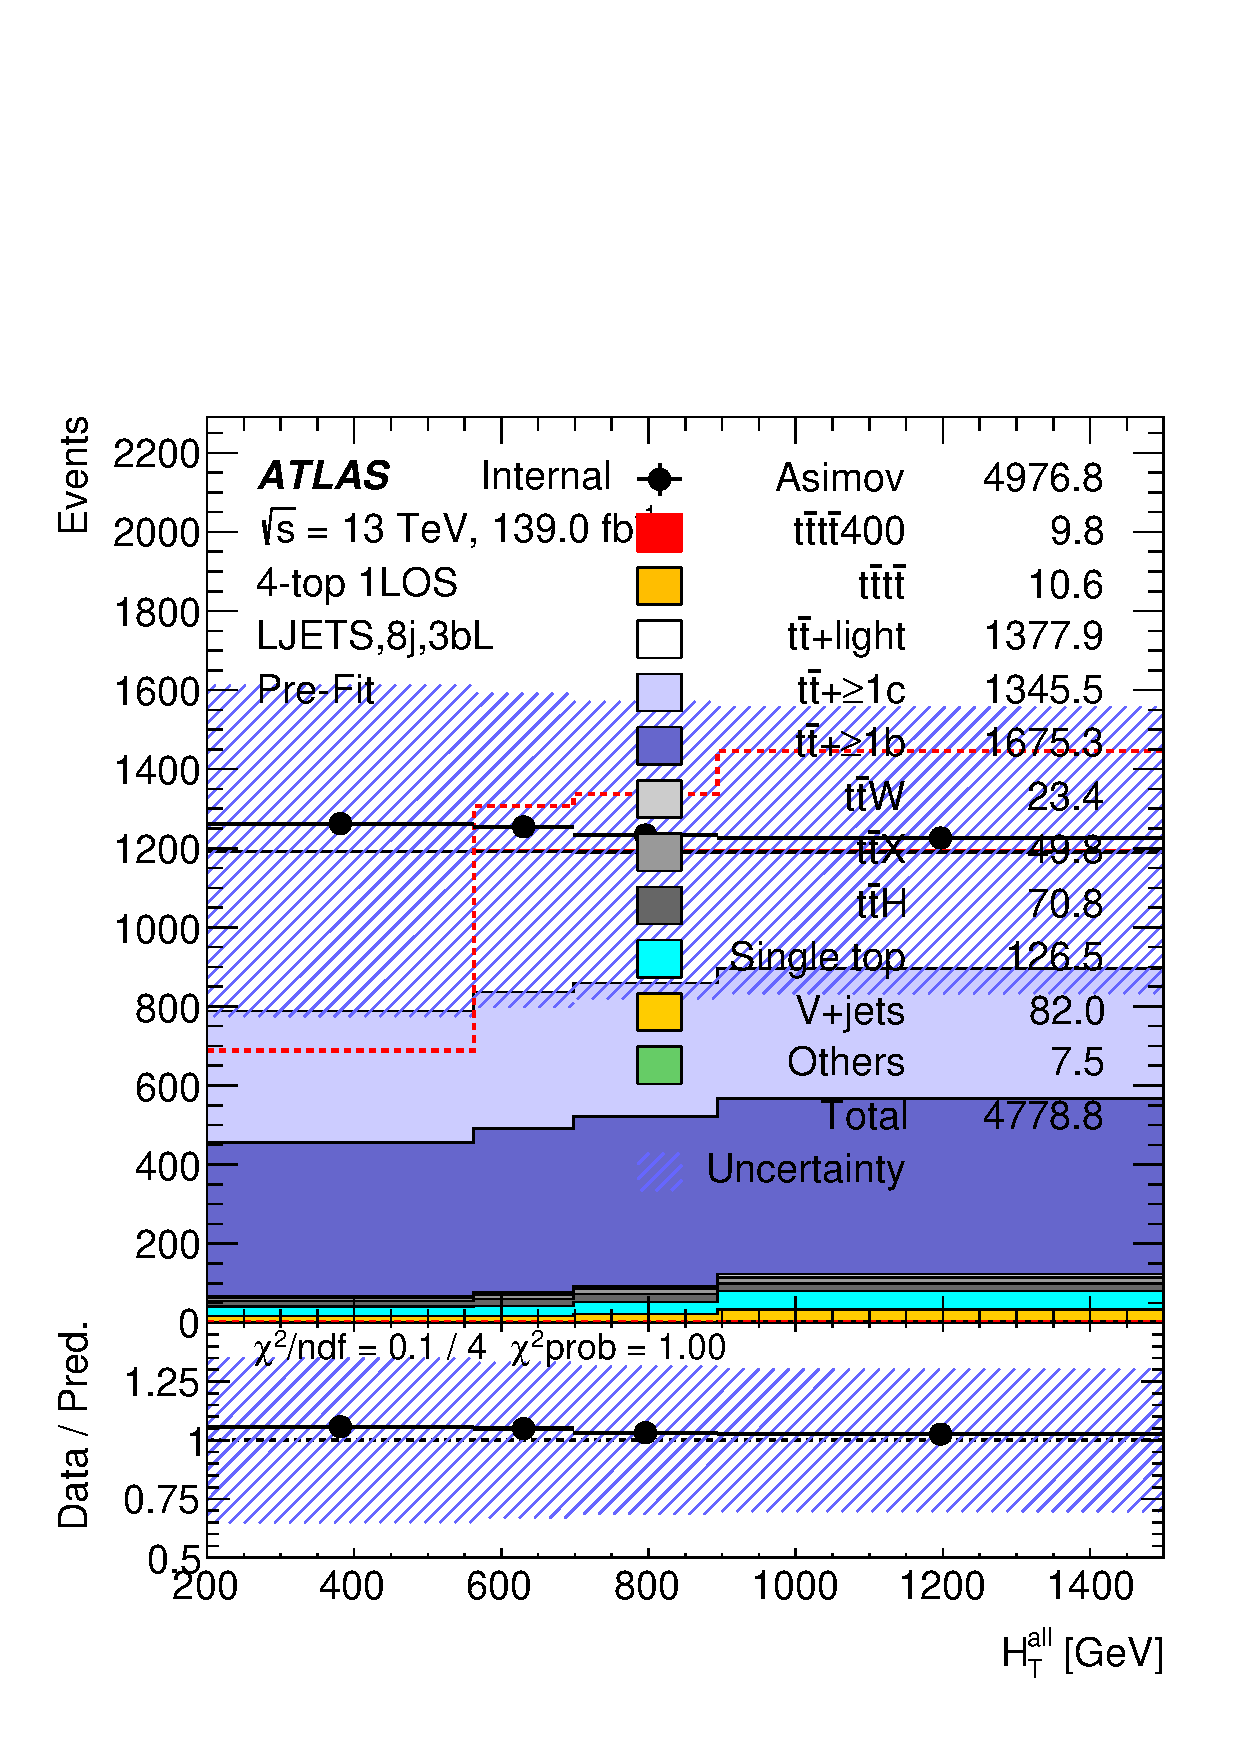
\includegraphics[width=0.23 \textwidth]{figures/4FS_studies/dataMC_4FSsyst_norew/ljets_8j3bL.pdf} &
        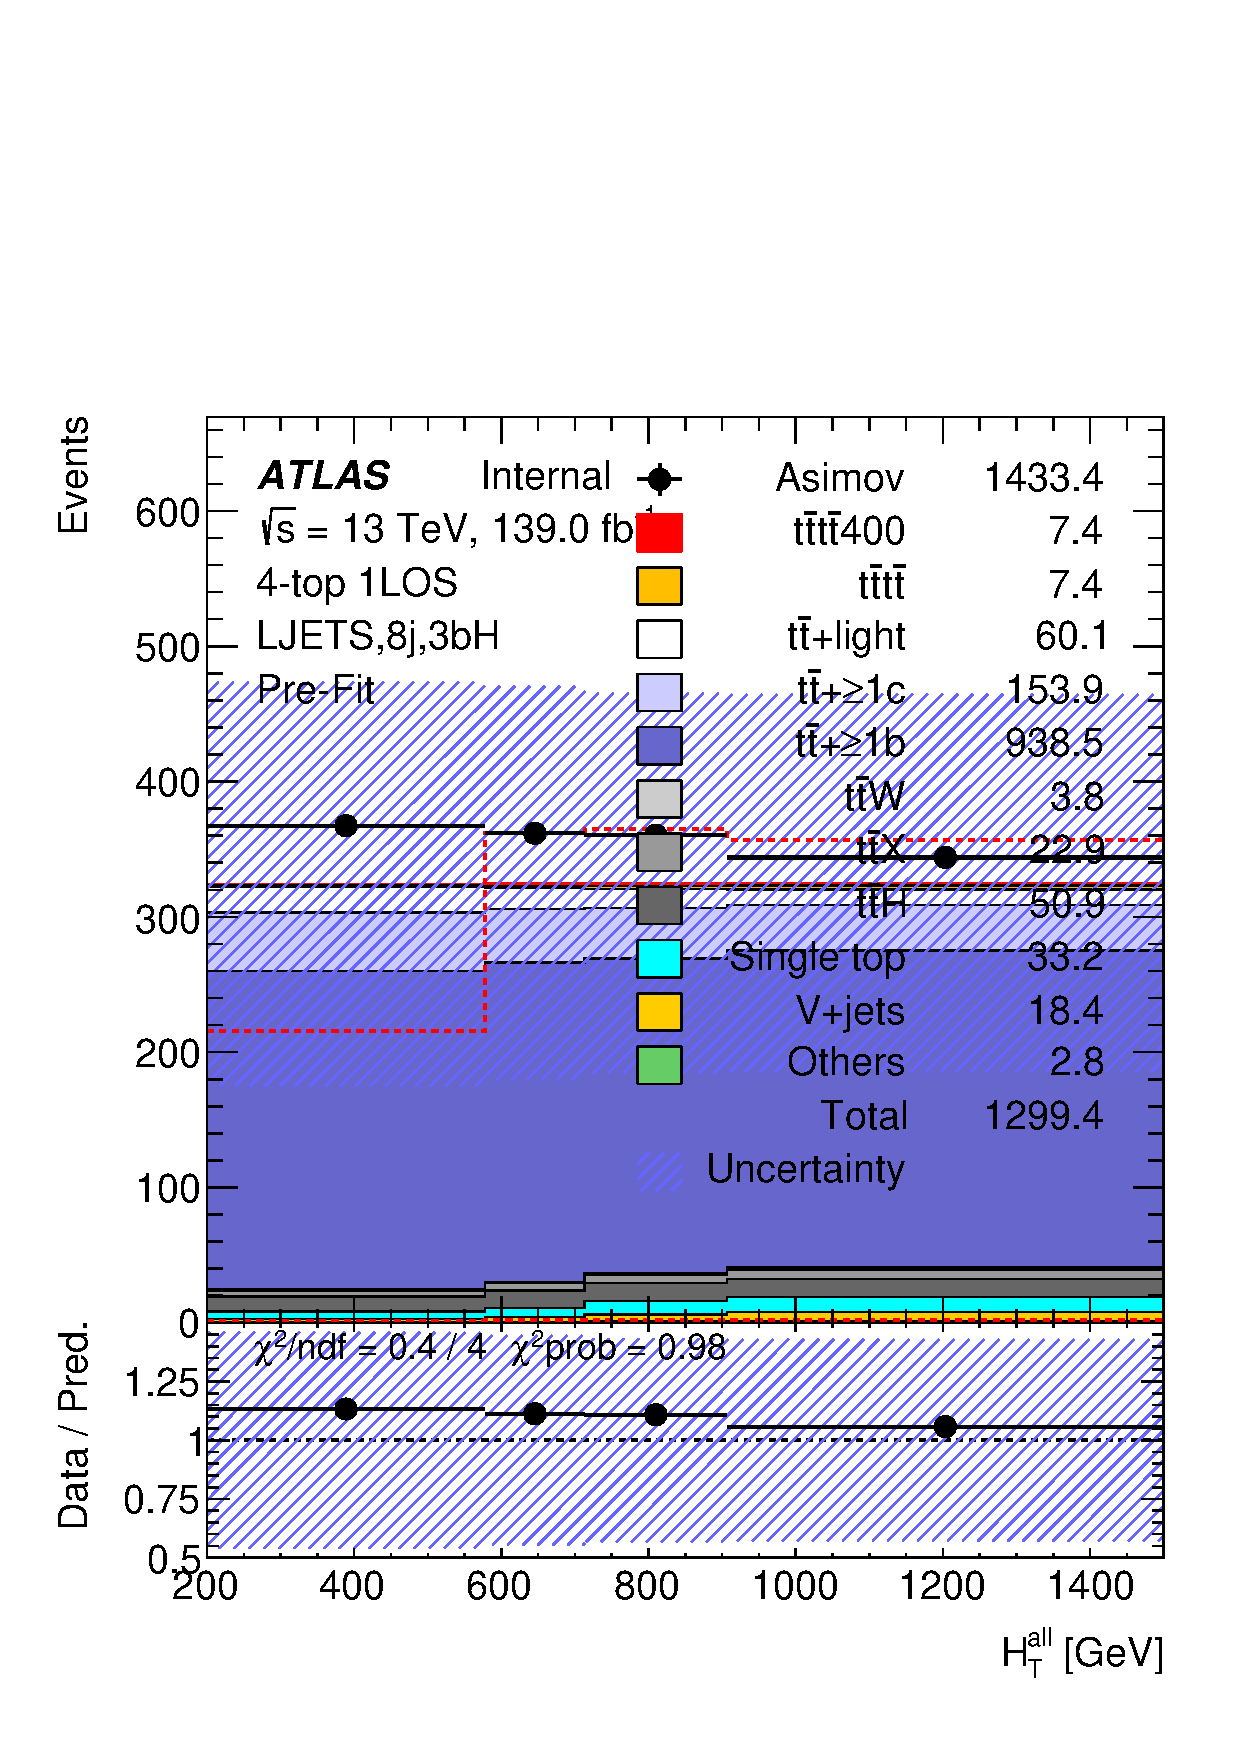
\includegraphics[width=0.23 \textwidth]{figures/4FS_studies/dataMC_4FSsyst_norew/ljets_8j3bH.pdf} &
        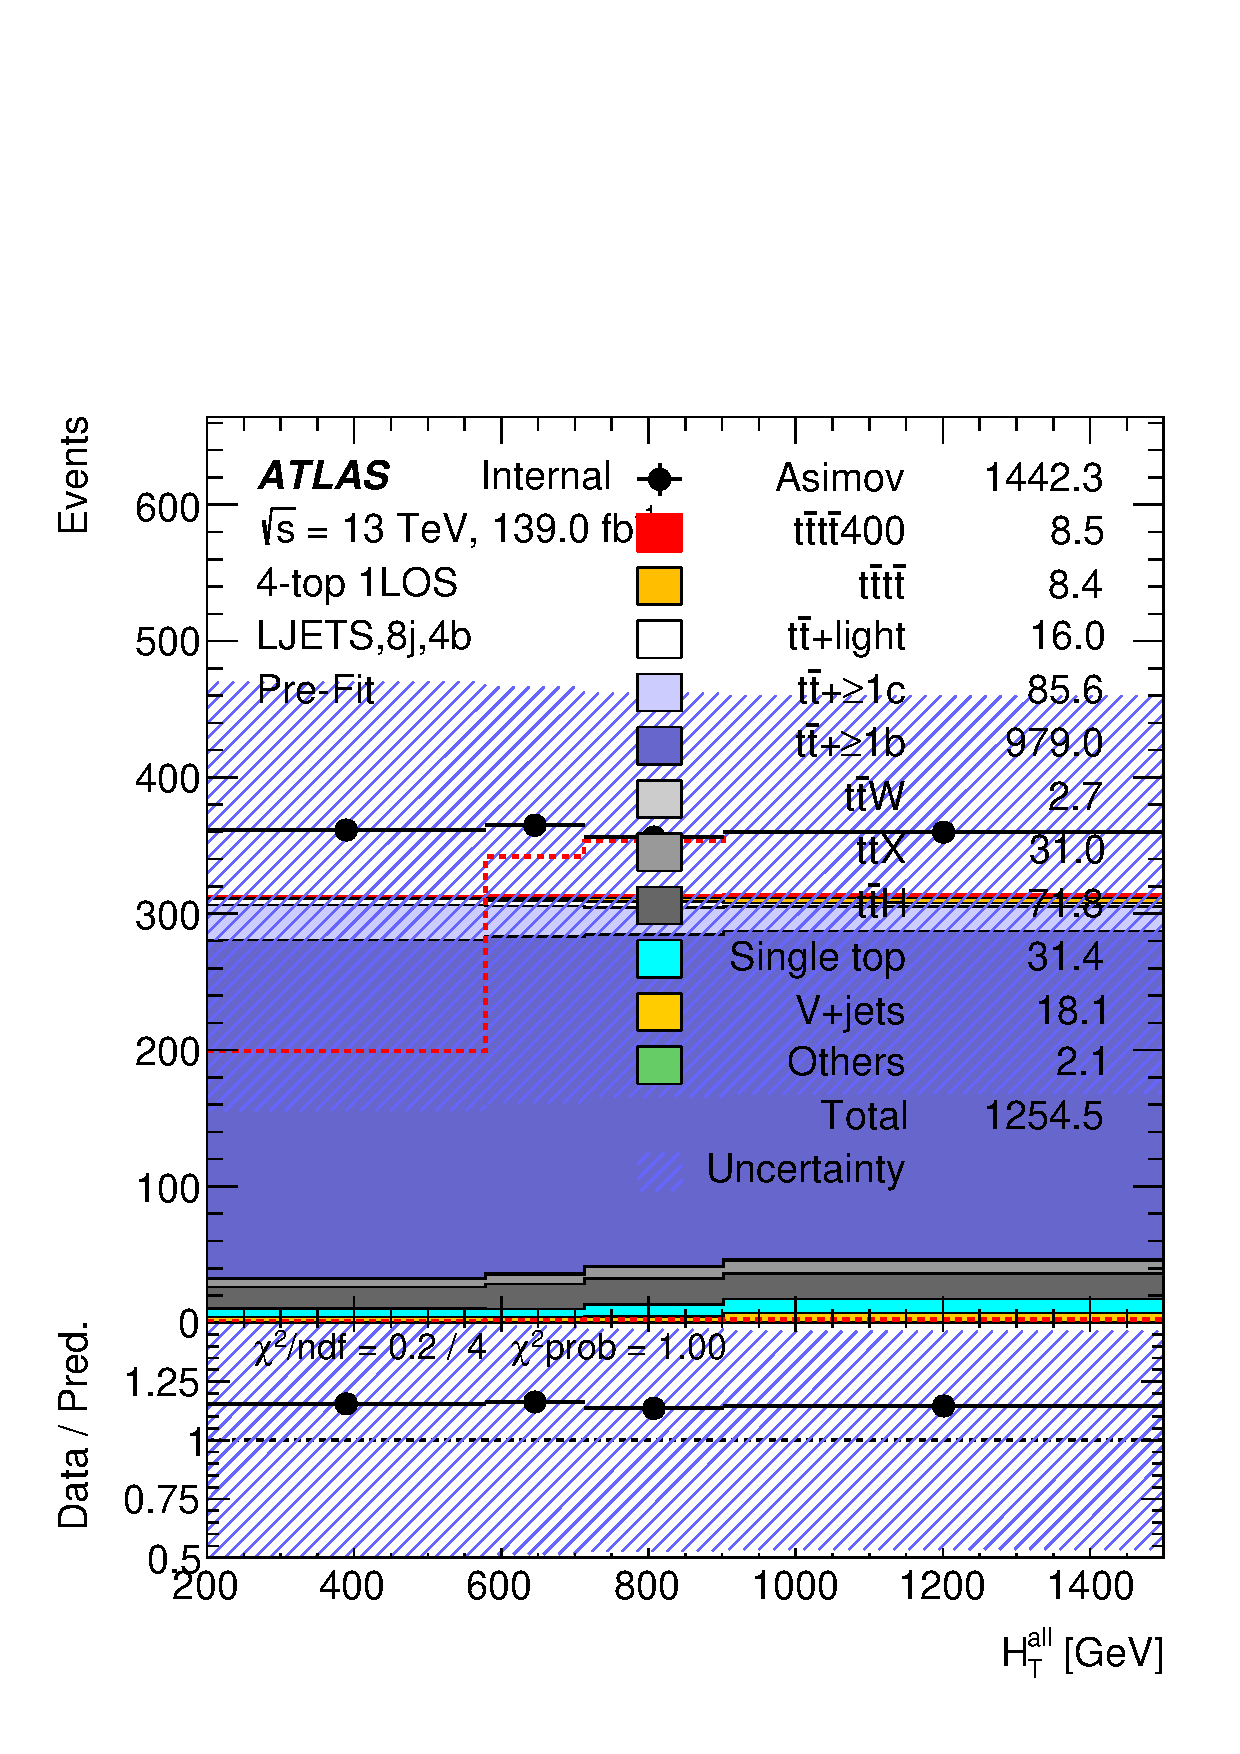
\includegraphics[width=0.23 \textwidth]{figures/4FS_studies/dataMC_4FSsyst_norew/ljets_8j4b.pdf} &
        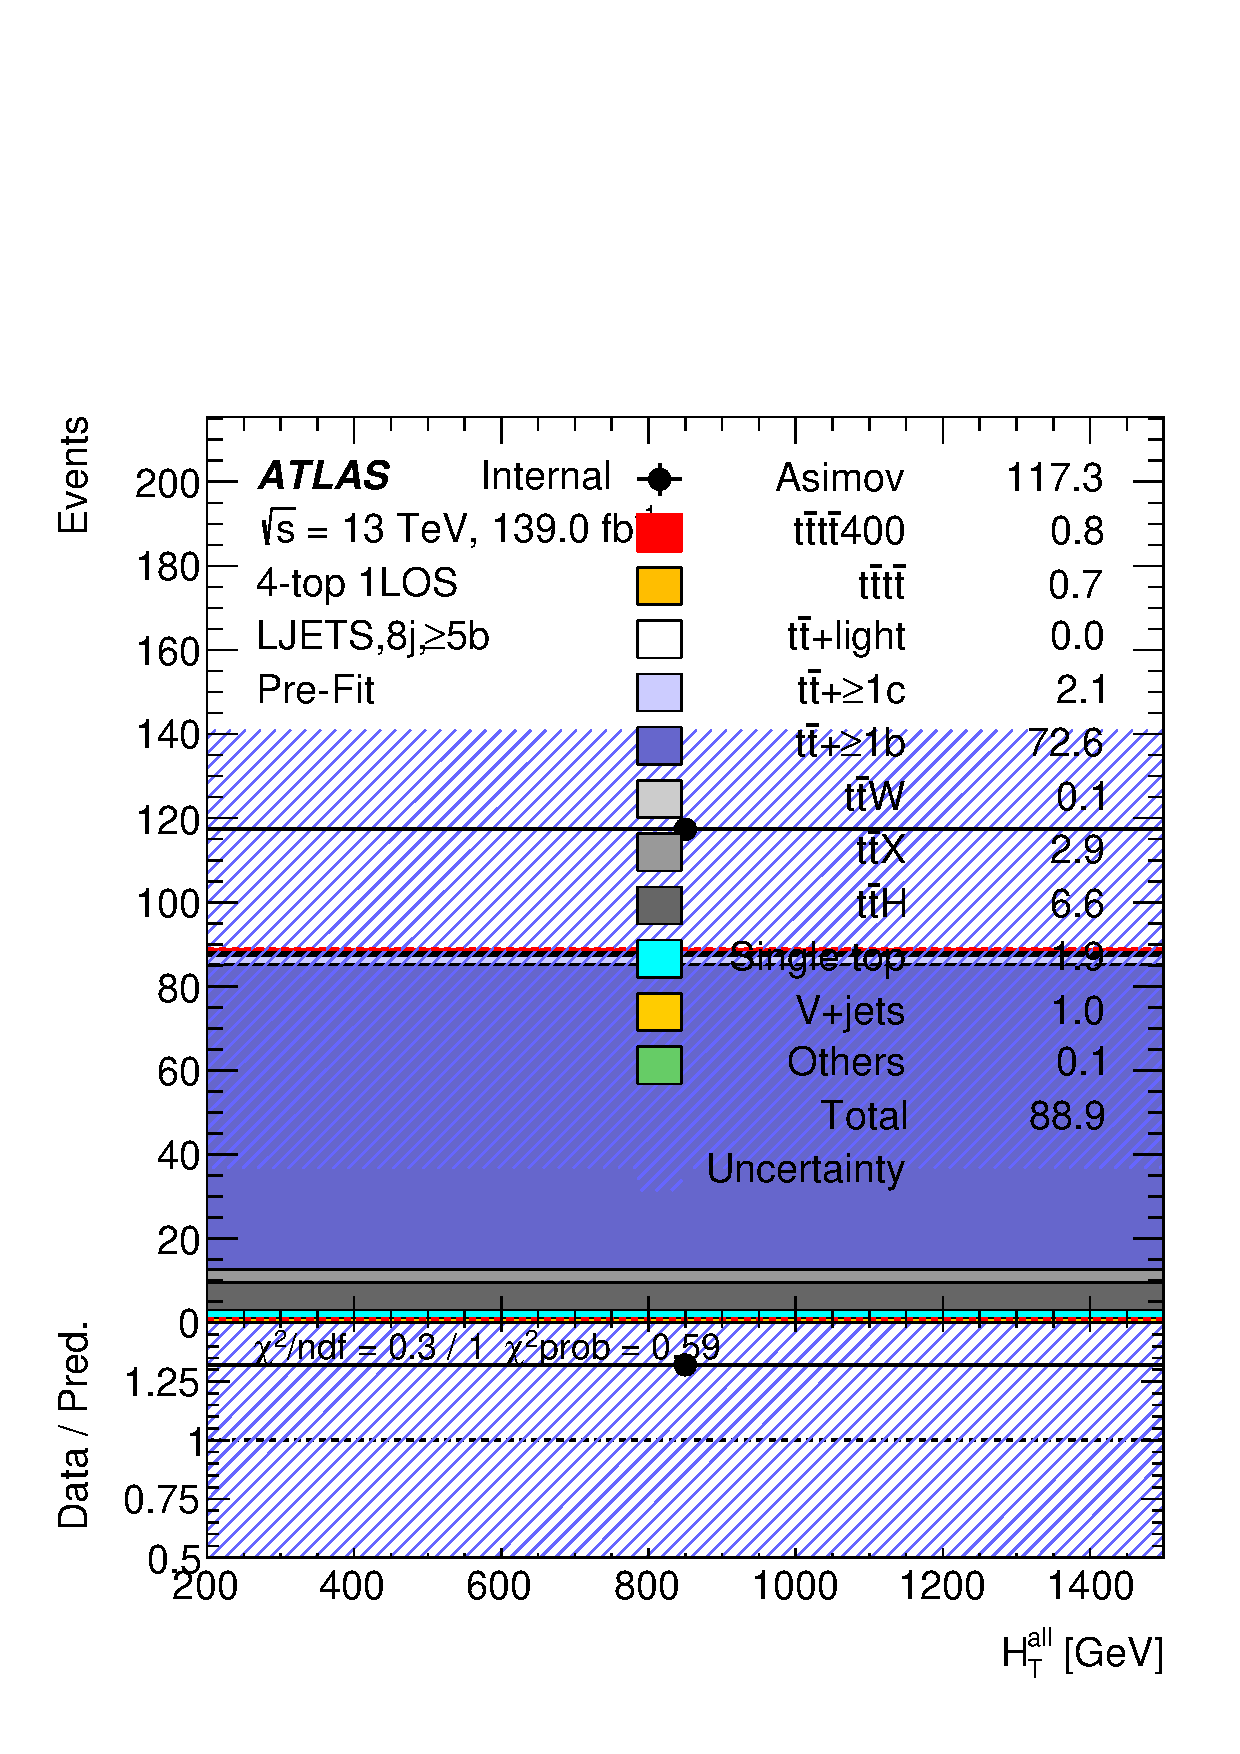
\includegraphics[width=0.23 \textwidth]{figures/4FS_studies/dataMC_4FSsyst_norew/ljets_8jge5b.pdf}\\

        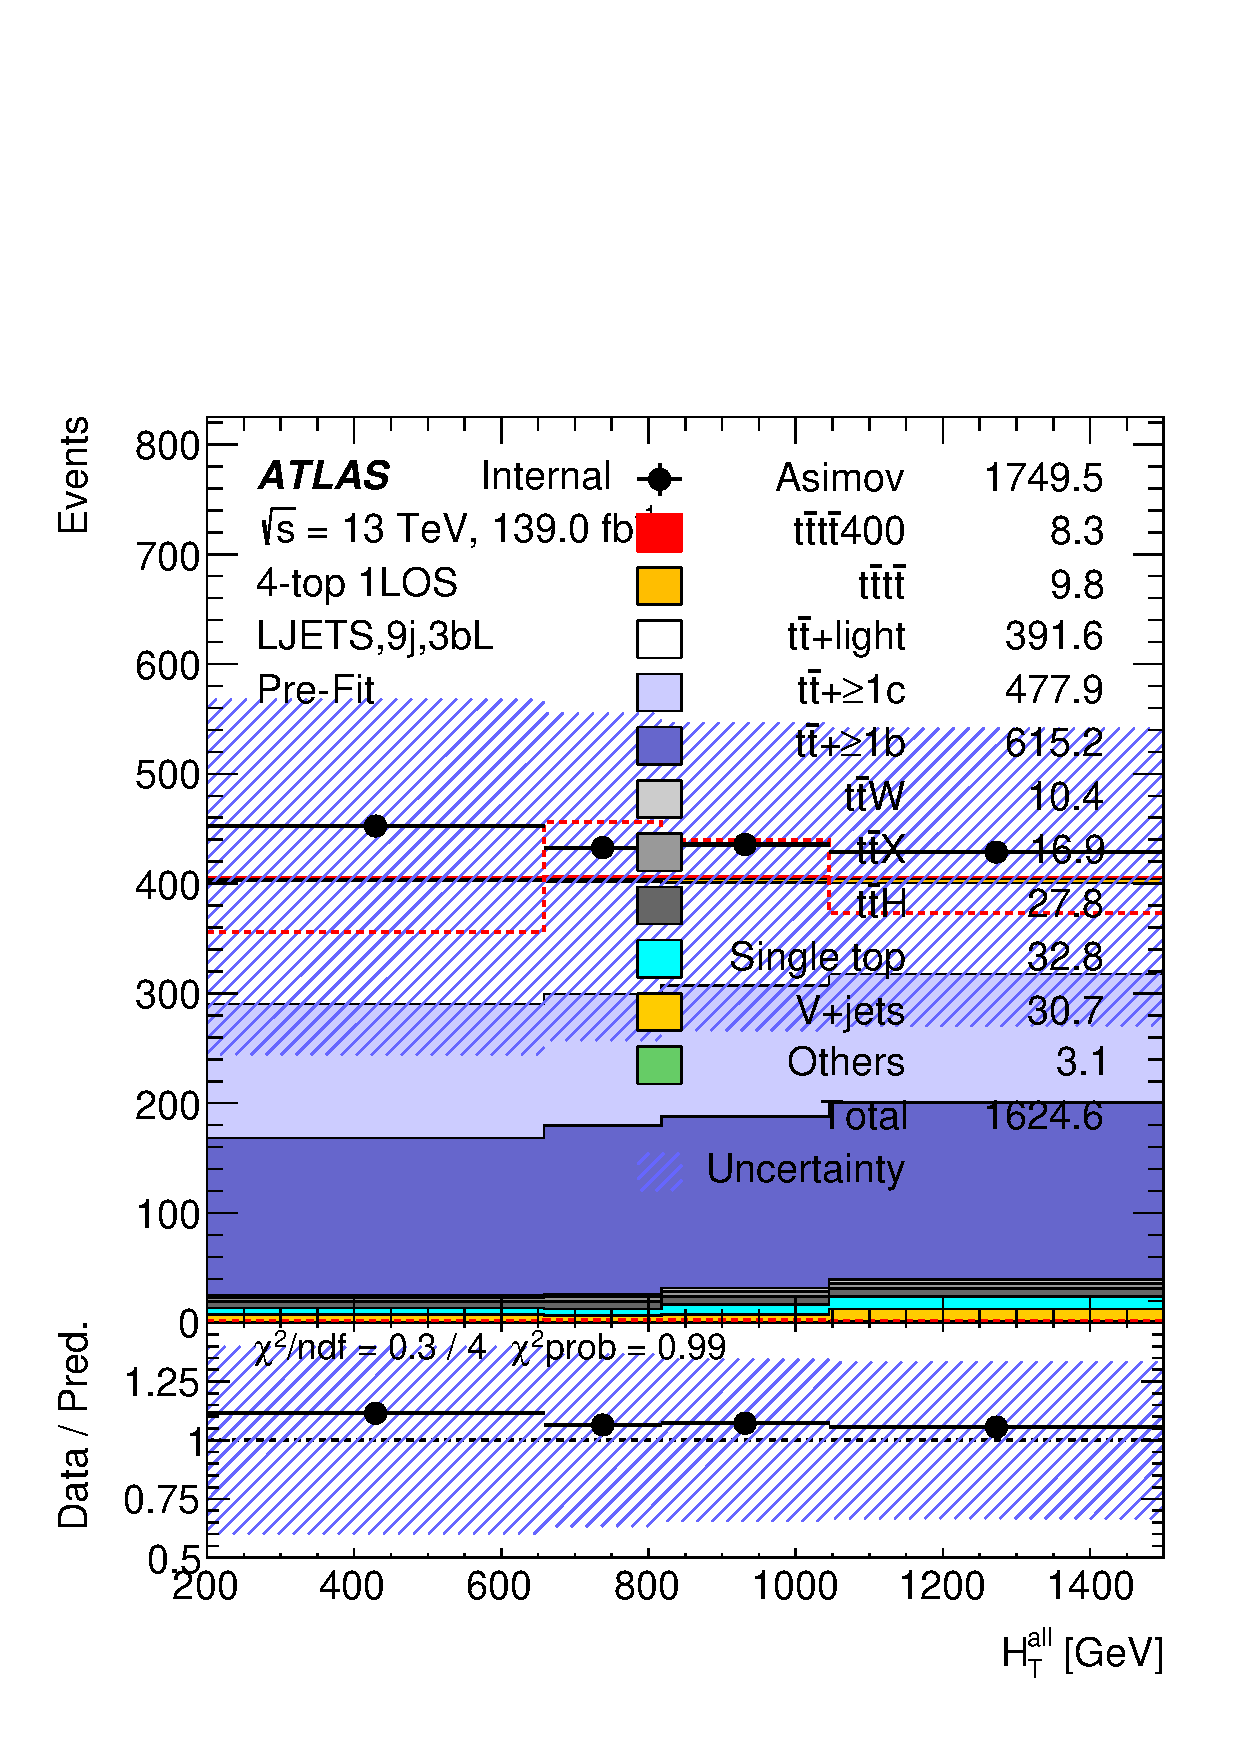
\includegraphics[width=0.23 \textwidth]{figures/4FS_studies/dataMC_4FSsyst_norew/ljets_9j3bL.pdf} &
        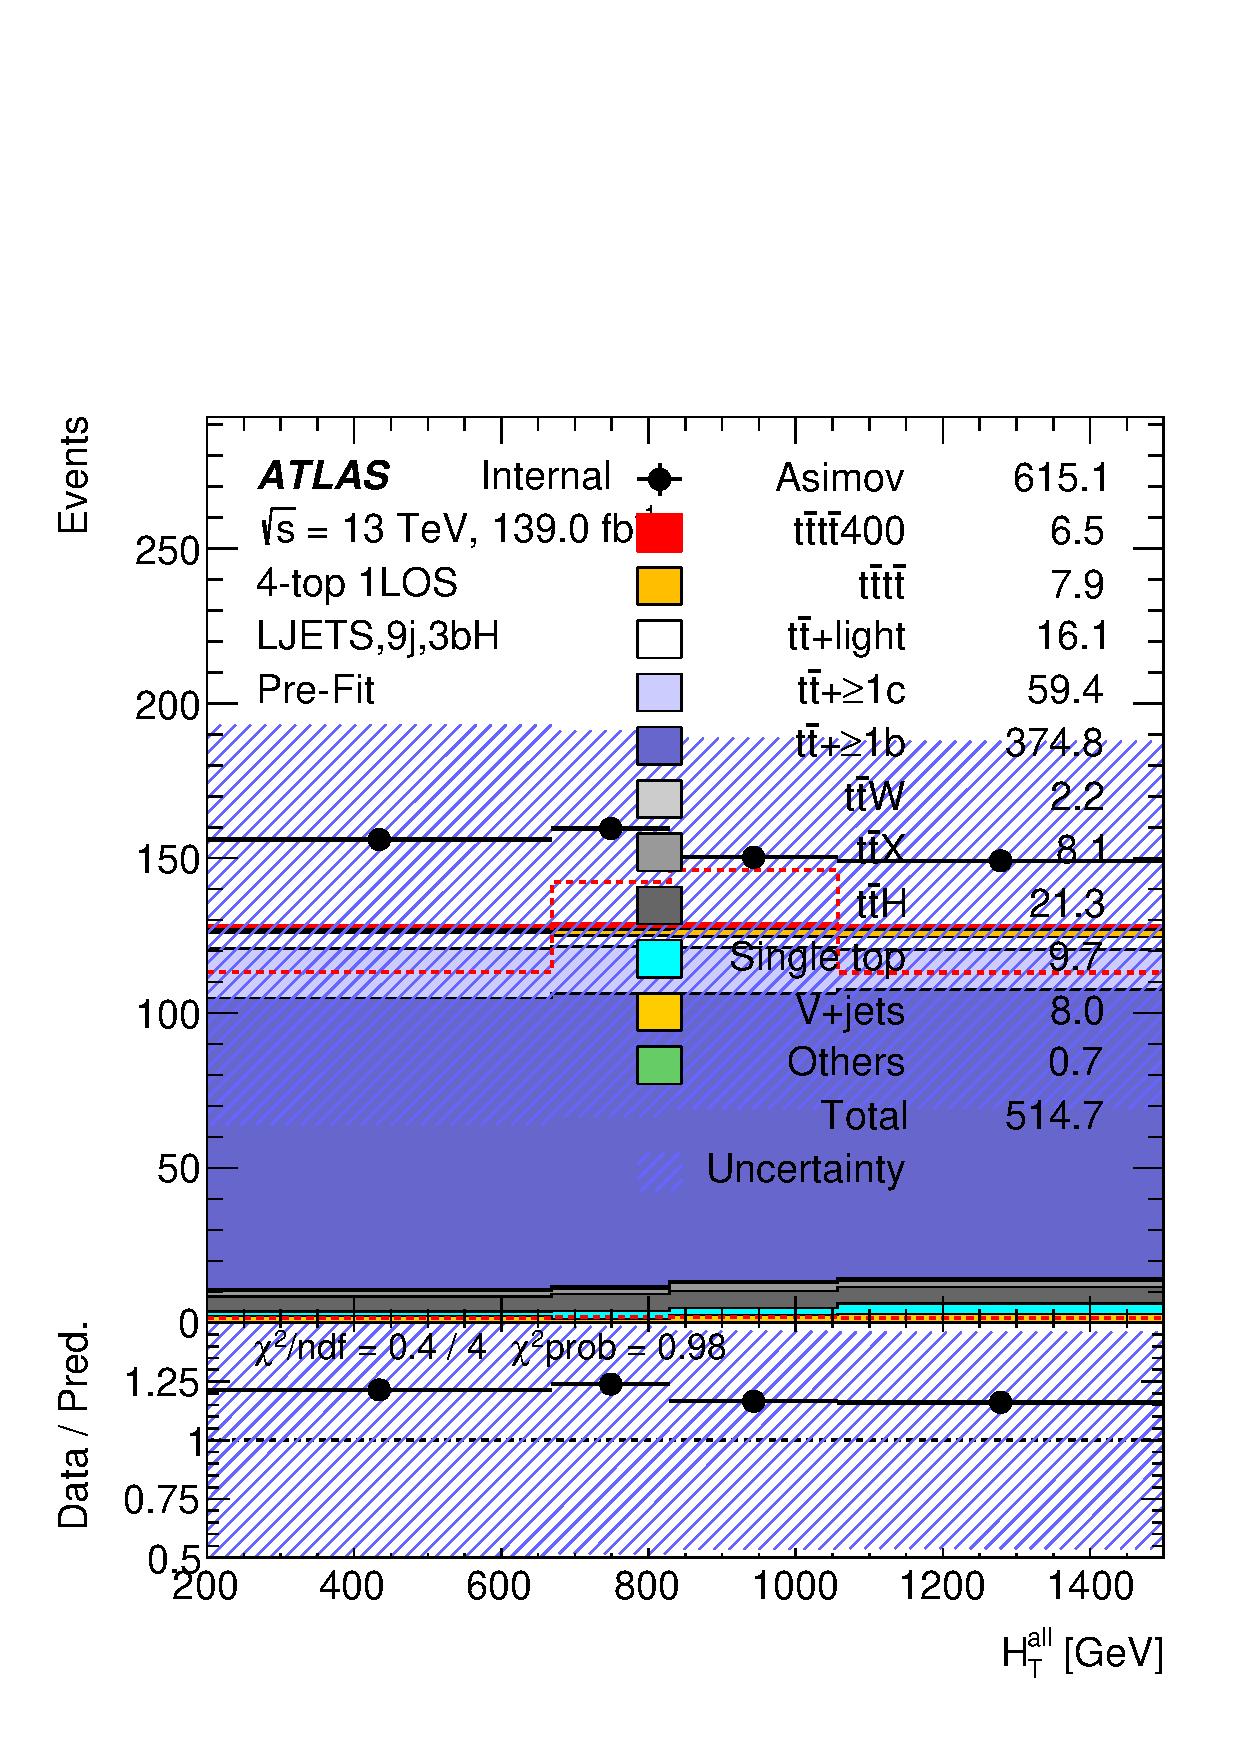
\includegraphics[width=0.23 \textwidth]{figures/4FS_studies/dataMC_4FSsyst_norew/ljets_9j3bH.pdf} &
        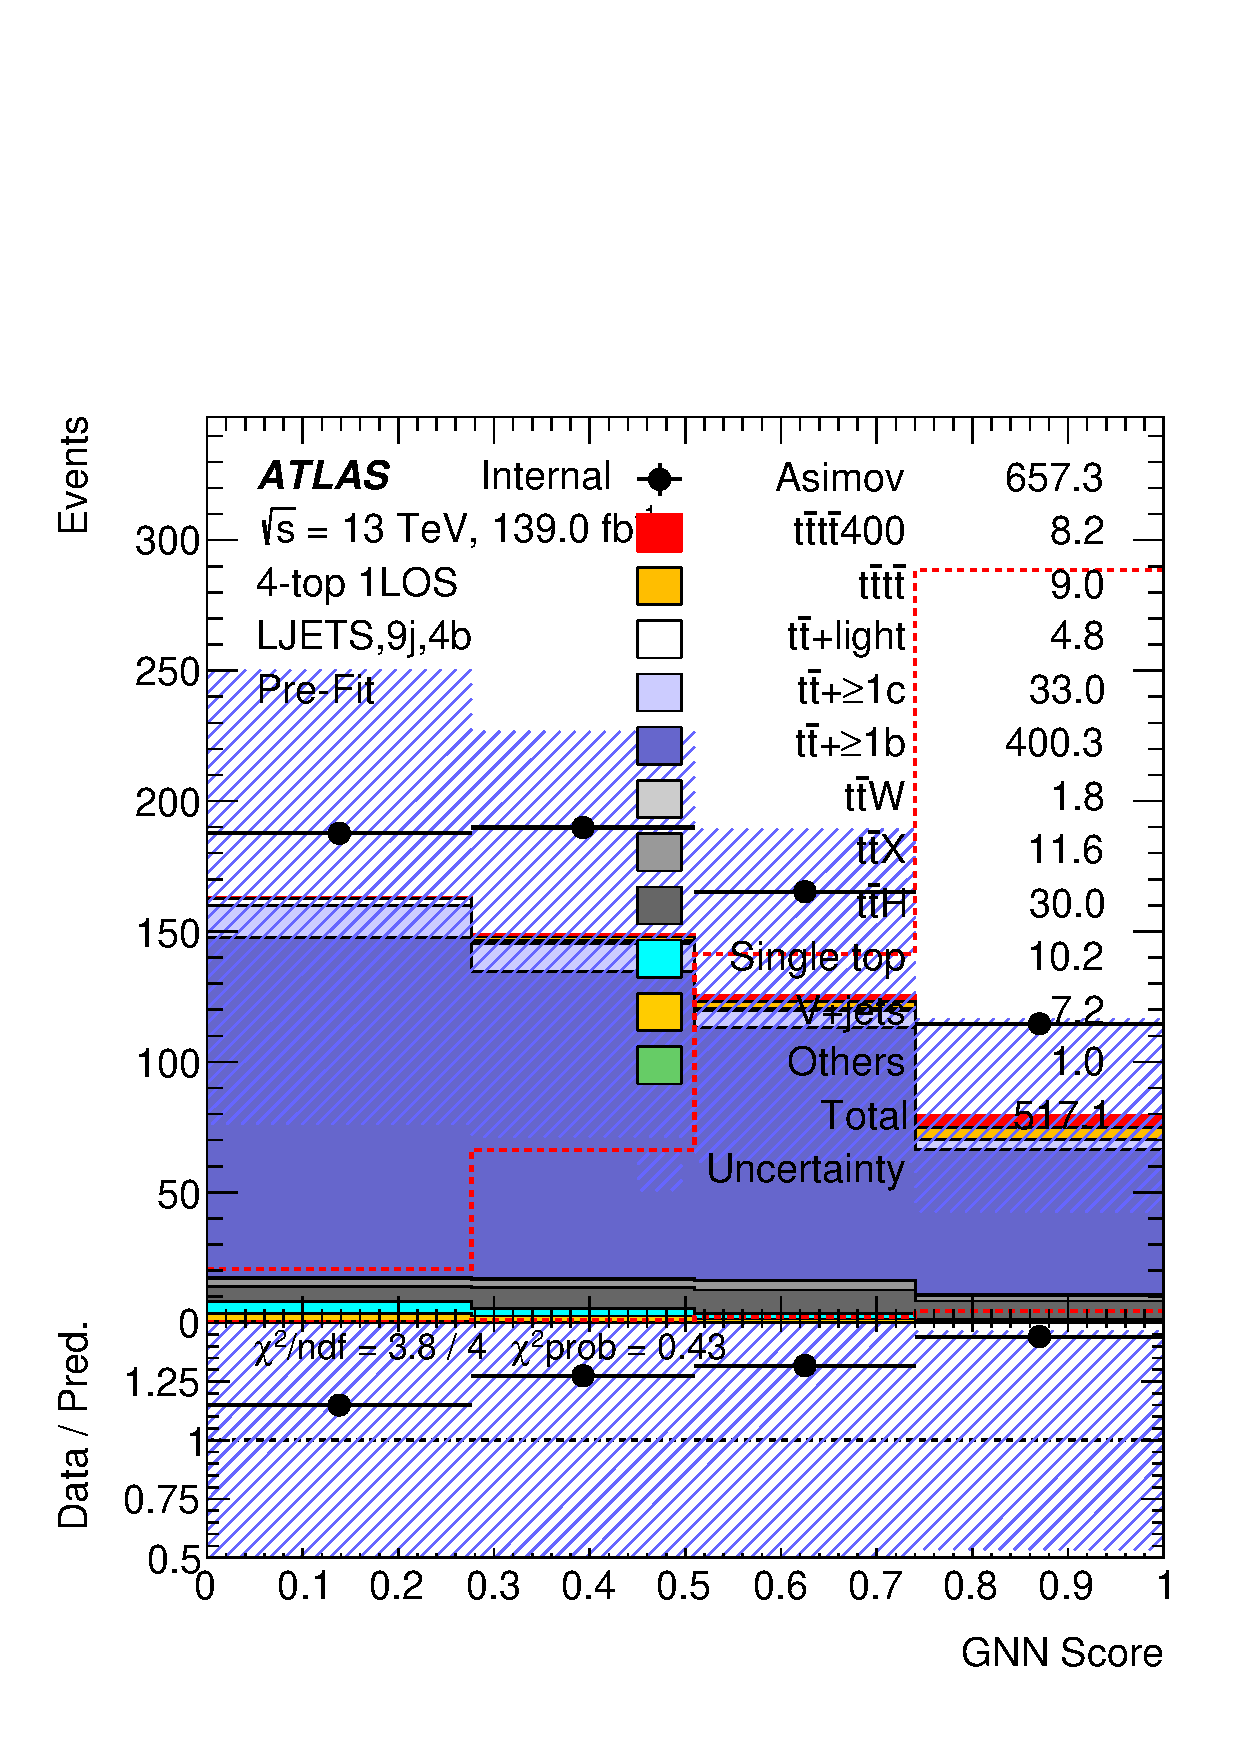
\includegraphics[width=0.23 \textwidth]{figures/4FS_studies/dataMC_4FSsyst_norew/ljets_9j4b.pdf} &
        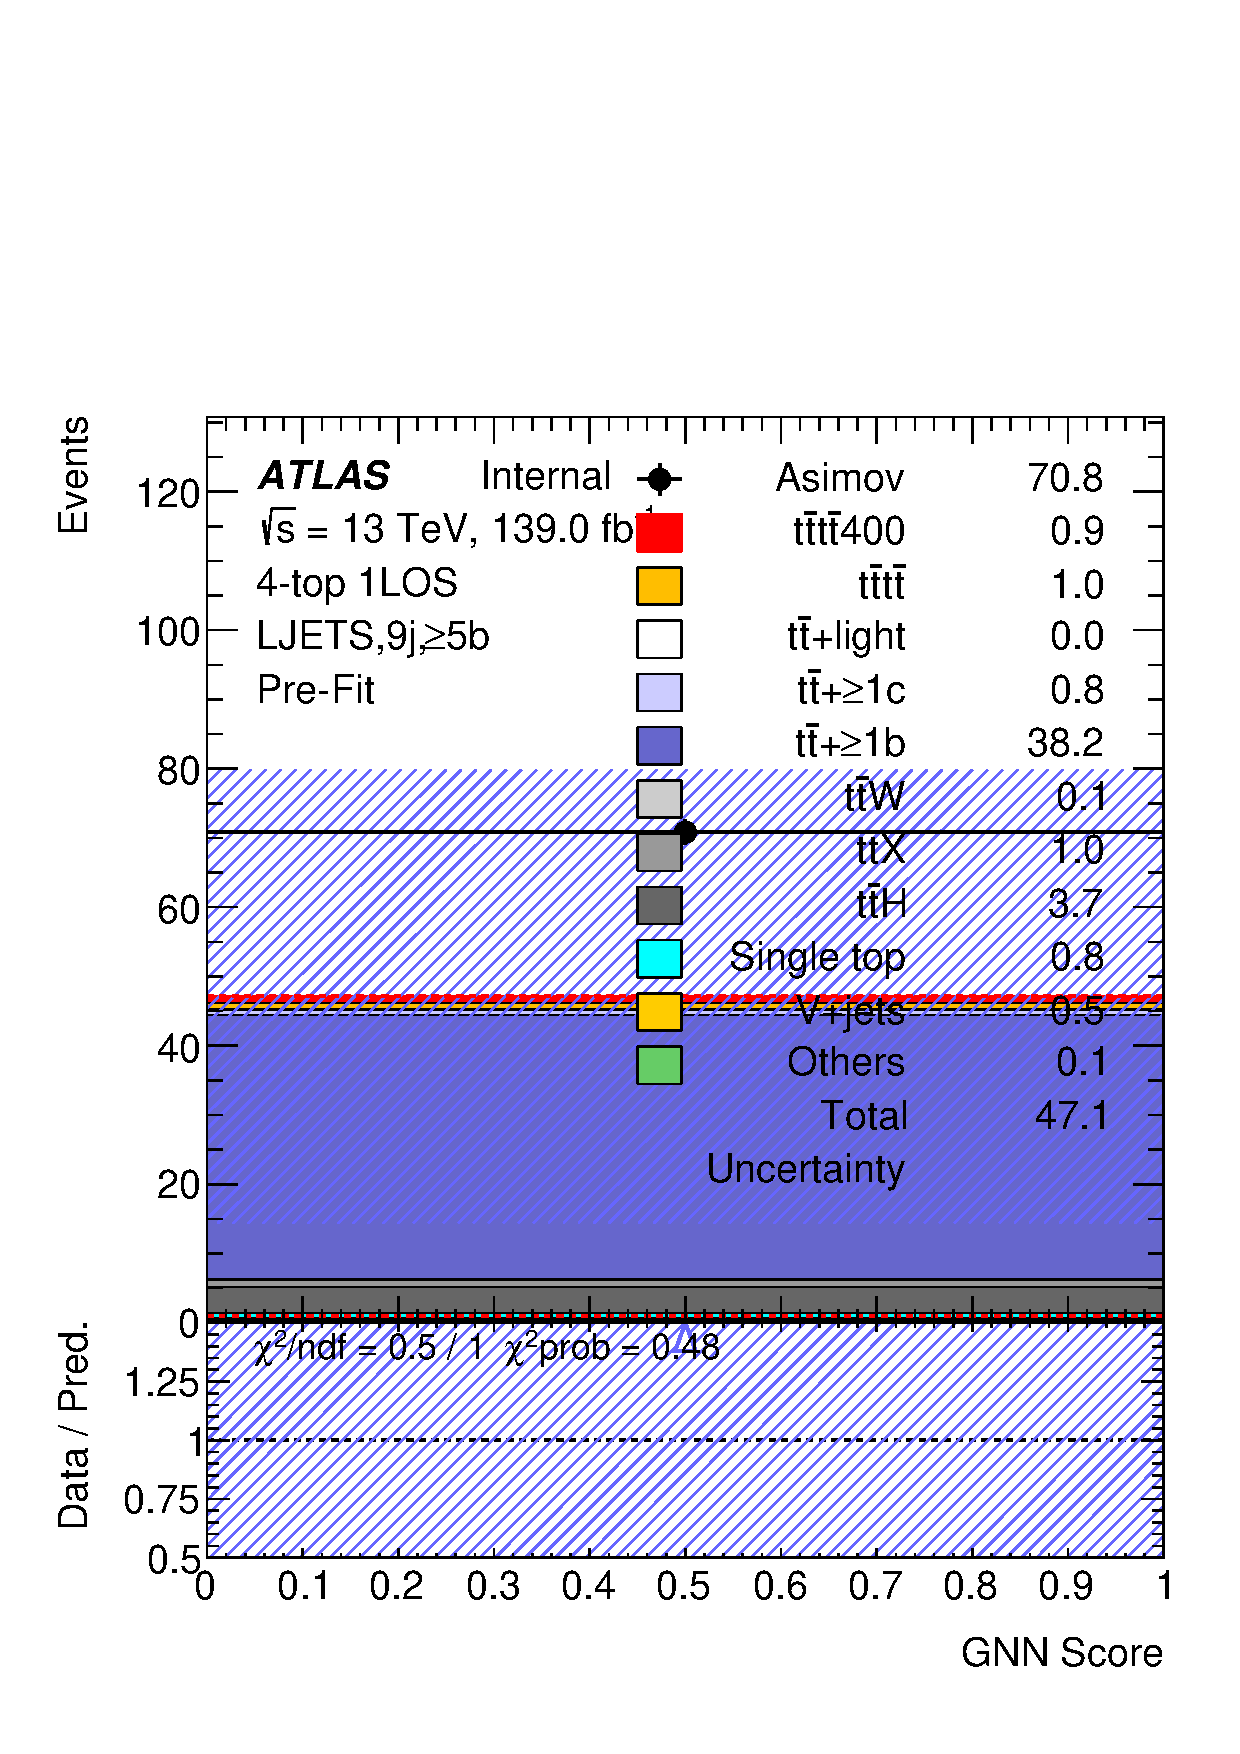
\includegraphics[width=0.23 \textwidth]{figures/4FS_studies/dataMC_4FSsyst_norew/ljets_9jge5b.pdf} \\

        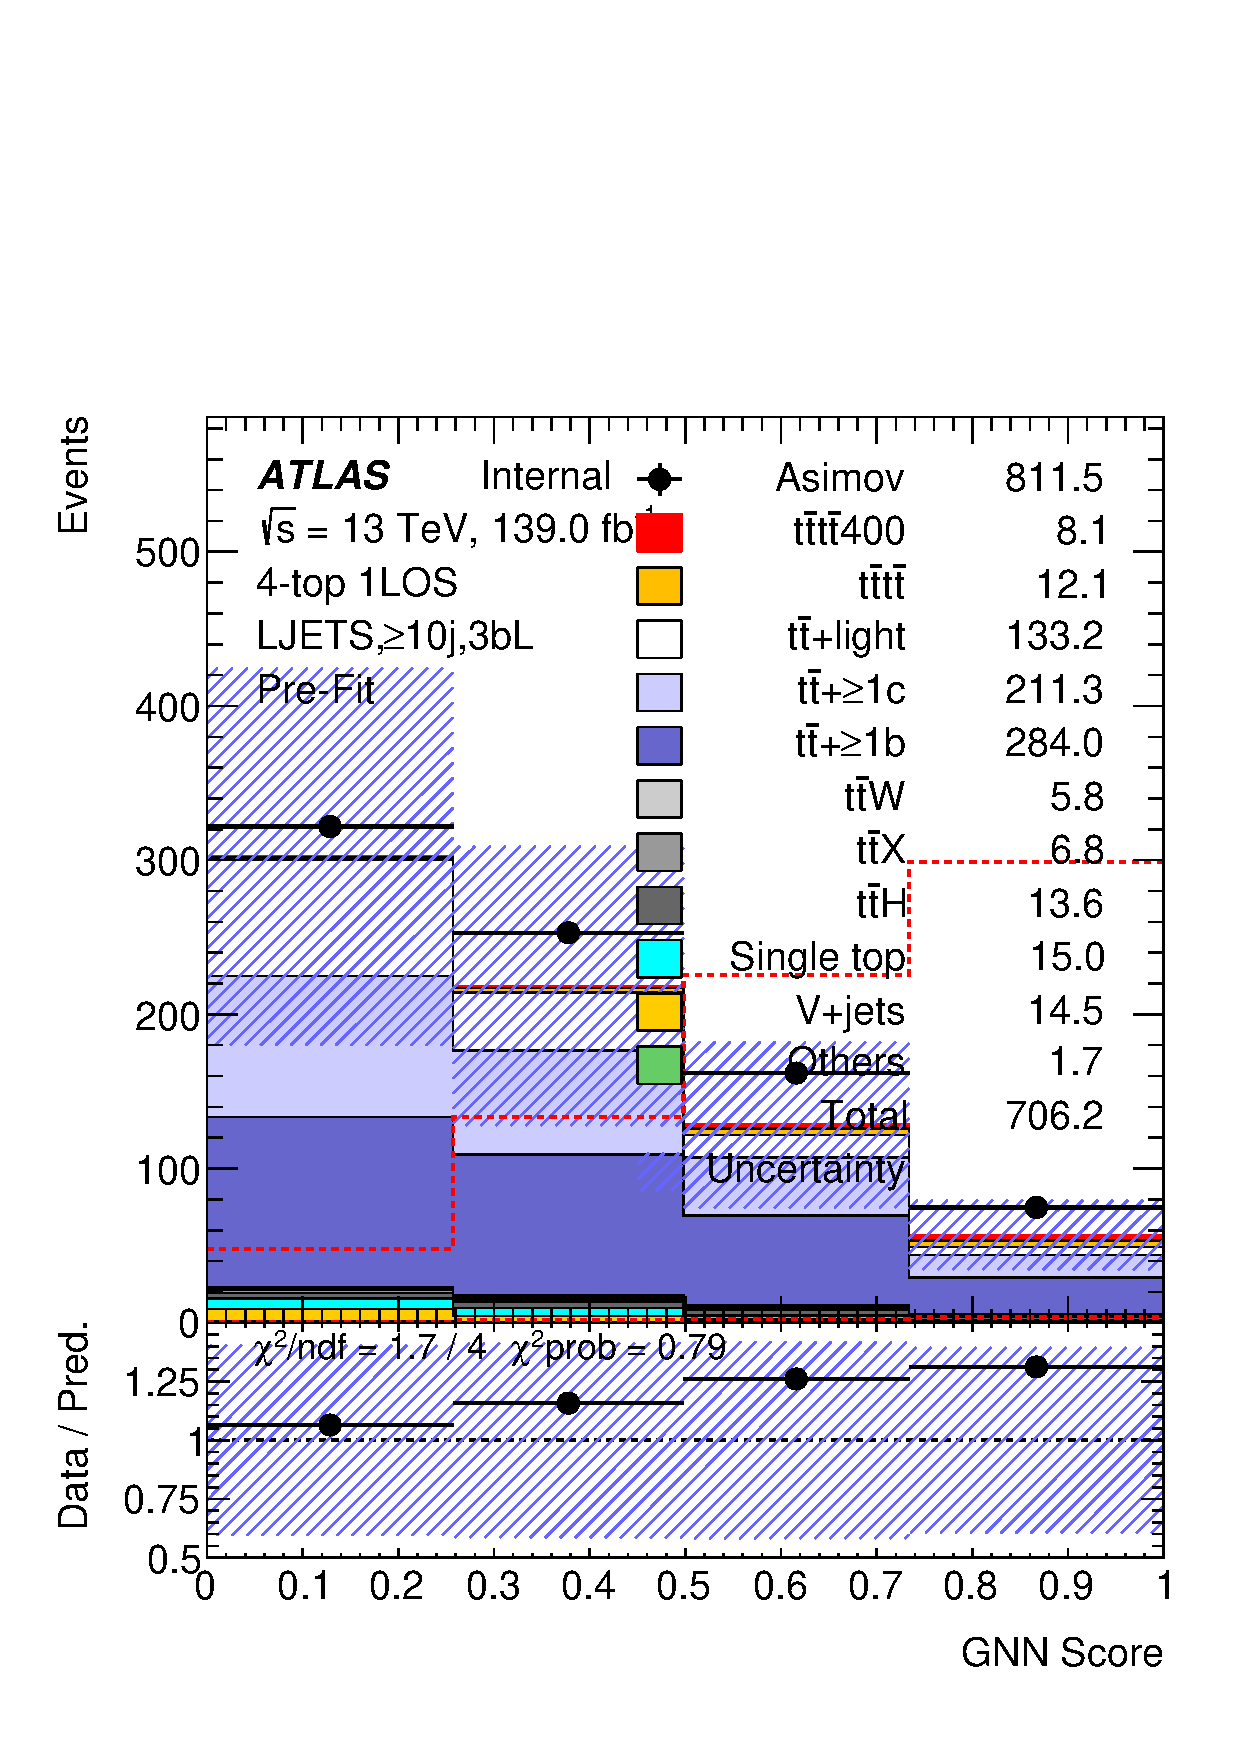
\includegraphics[width=0.23 \textwidth]{figures/4FS_studies/dataMC_4FSsyst_norew/ljets_ge10j3bL.pdf} &
        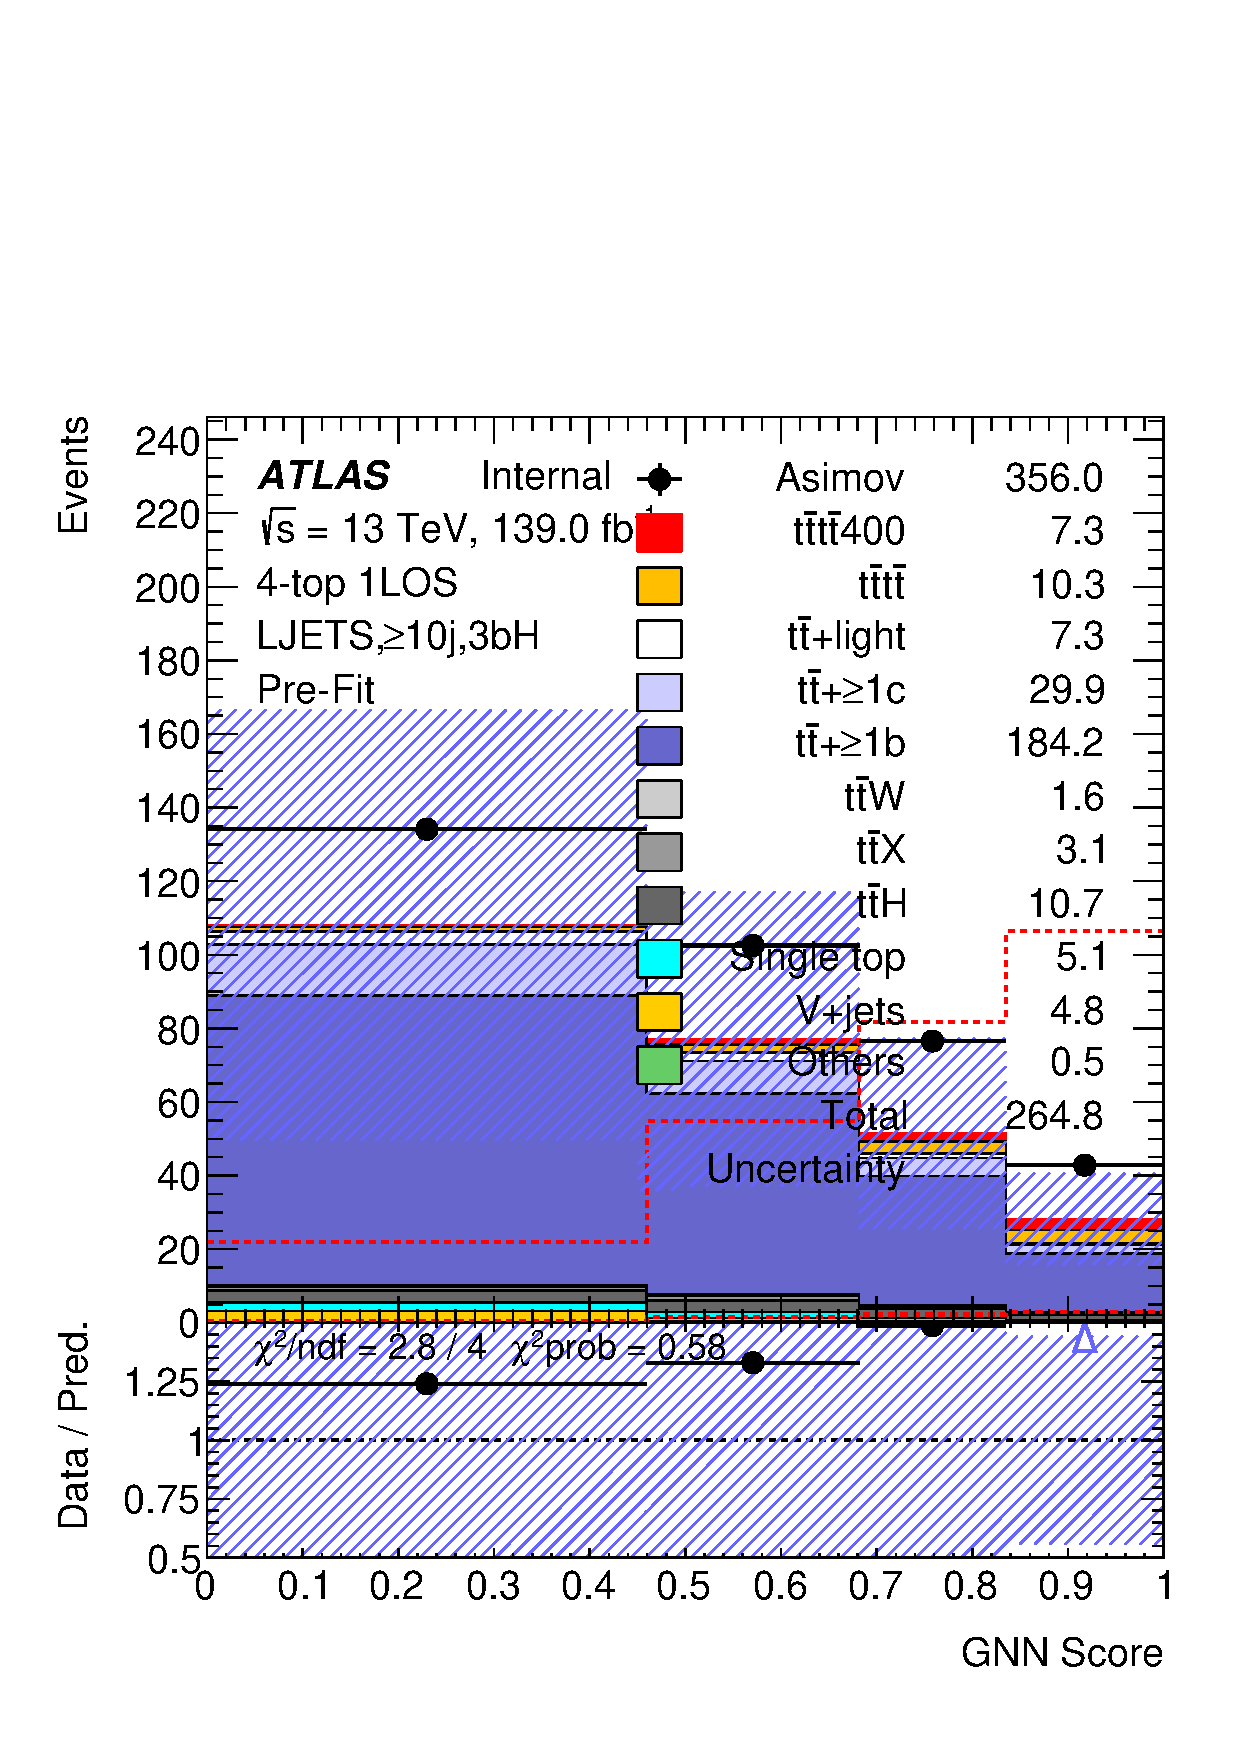
\includegraphics[width=0.23 \textwidth]{figures/4FS_studies/dataMC_4FSsyst_norew/ljets_ge10j3bH.pdf} &
        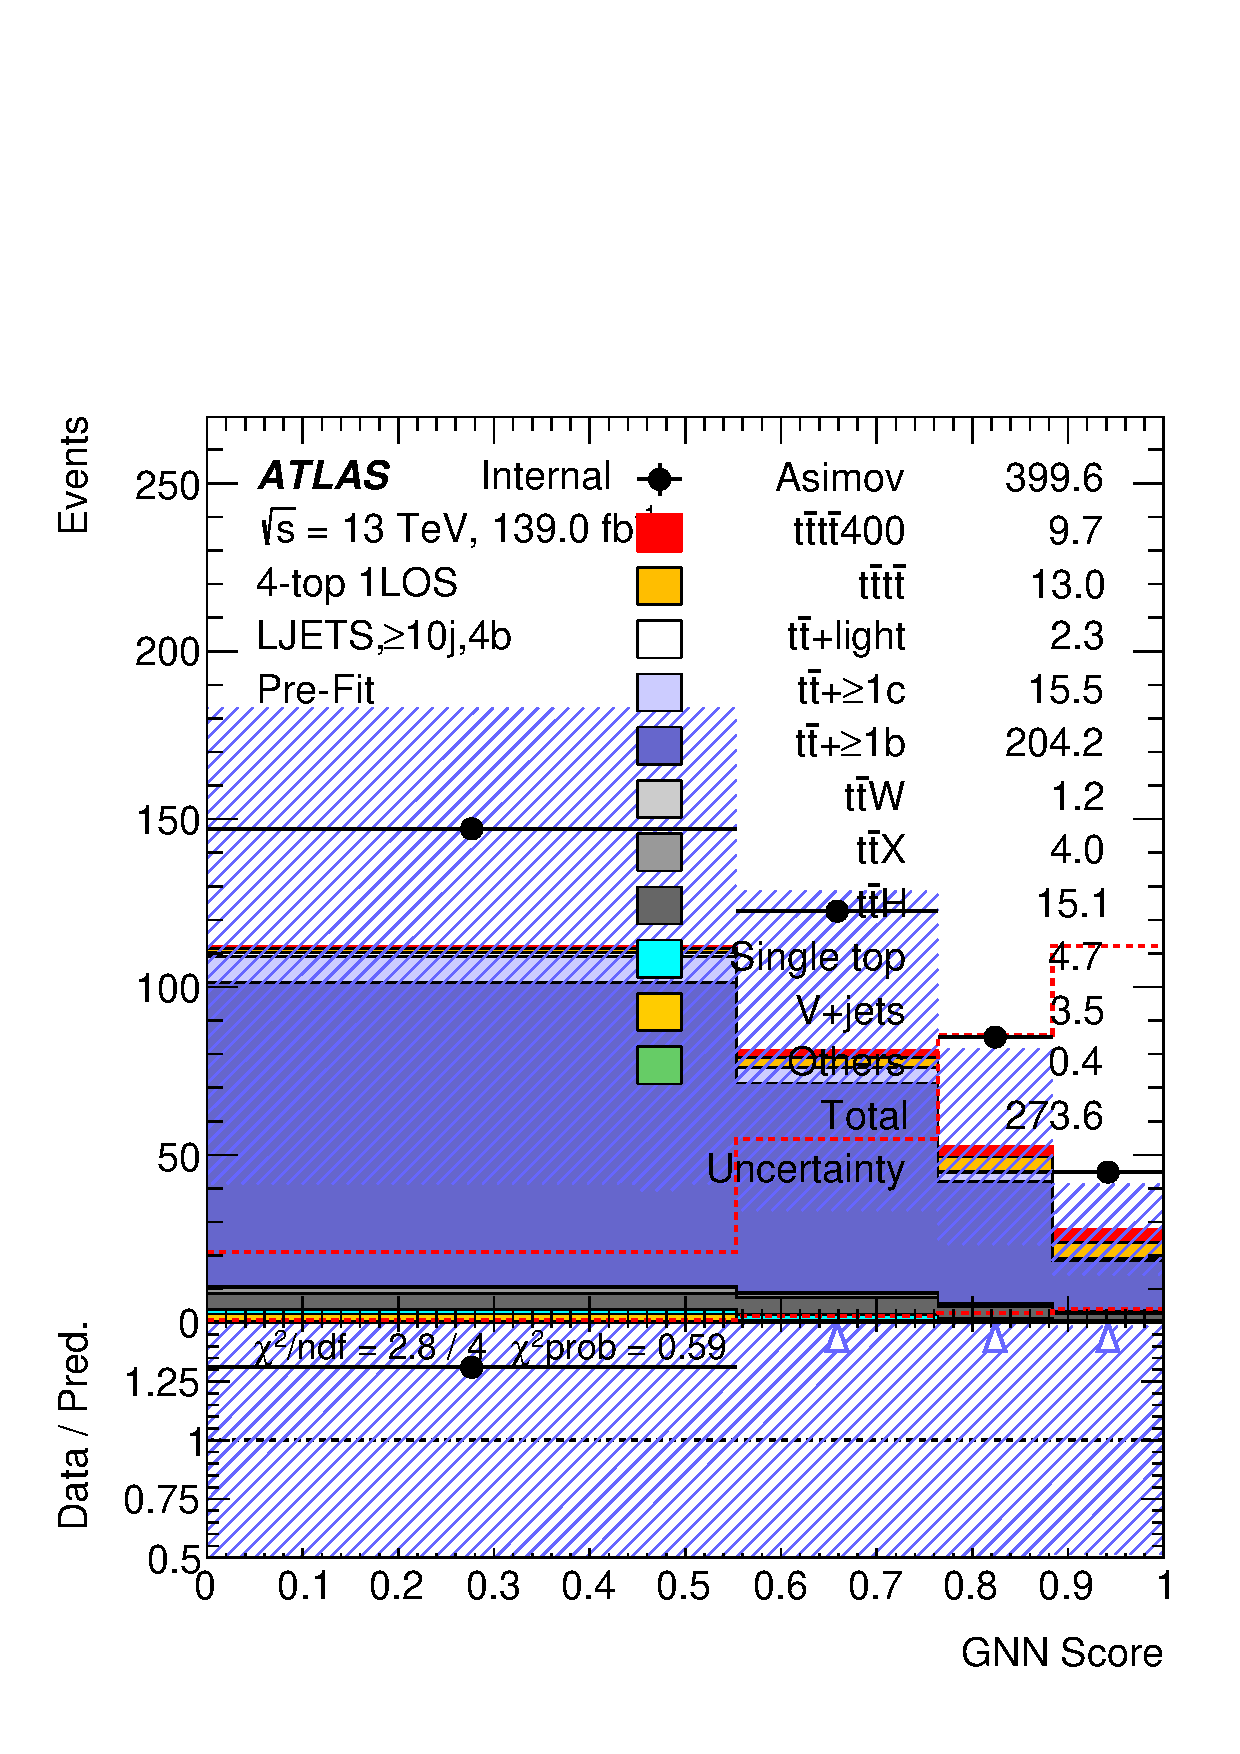
\includegraphics[width=0.23 \textwidth]{figures/4FS_studies/dataMC_4FSsyst_norew/ljets_ge10j4b.pdf} &
        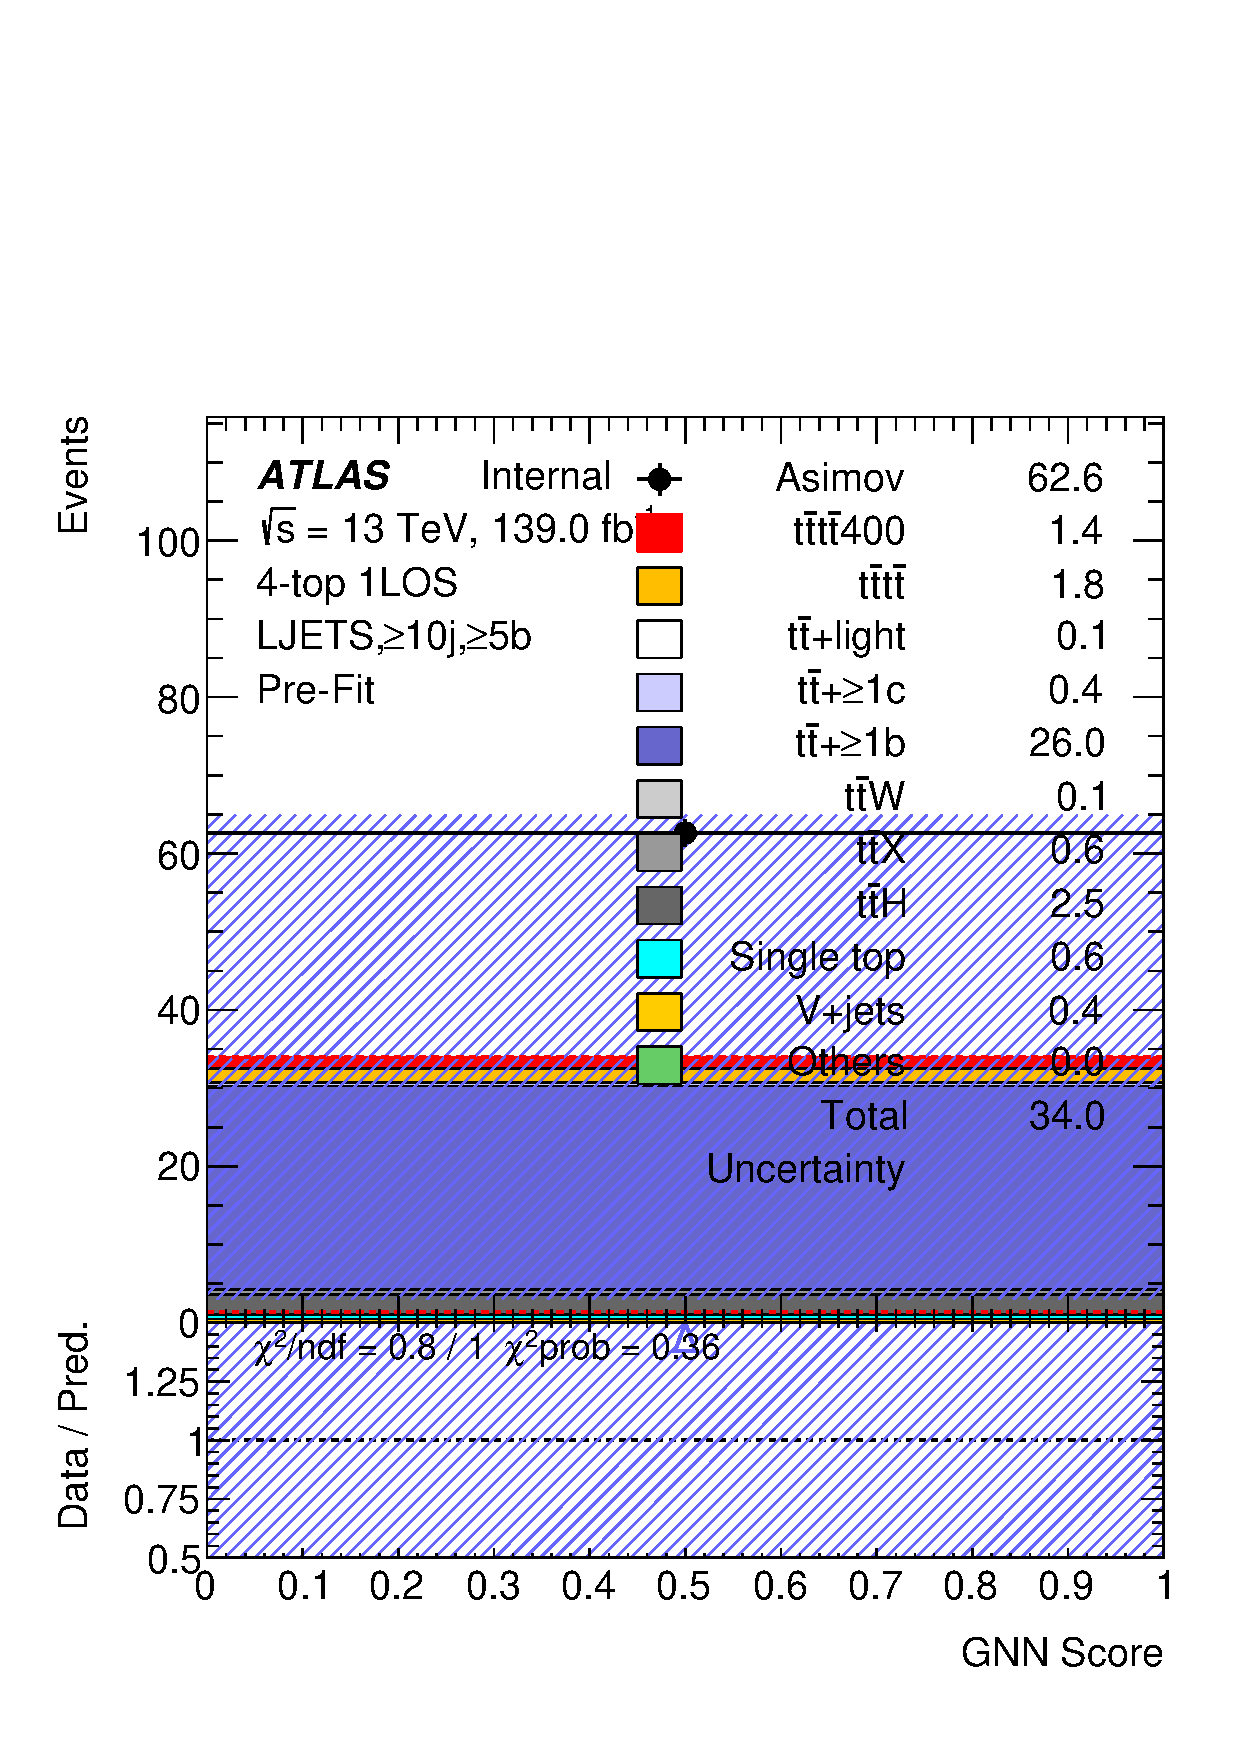
\includegraphics[width=0.23 \textwidth]{figures/4FS_studies/dataMC_4FSsyst_norew/ljets_ge10jge5b.pdf} \\
        \end{tabular}
        \caption{\label{fig:4FS_dataMC_4FSsyst_norew_1L_prefit}Pre-fit comparison of the 1L regions between samples with $t\bar{t}$ TTB samples produced with 5FS (MC) and $t\bar{t}$ TTB samples produced with 4FS (set as `pseudodata'). All systematics including 4FS systematics are incorporated in the uncertainty. The $t\bar{t}$ samples are not reweighted.}
\end{center}
\end{figure}

\begin{figure}[htbp!]
        \begin{center} \setlength{\tabcolsep}{2.5pt}\footnotesize
        \begin{tabular}{ccc}
        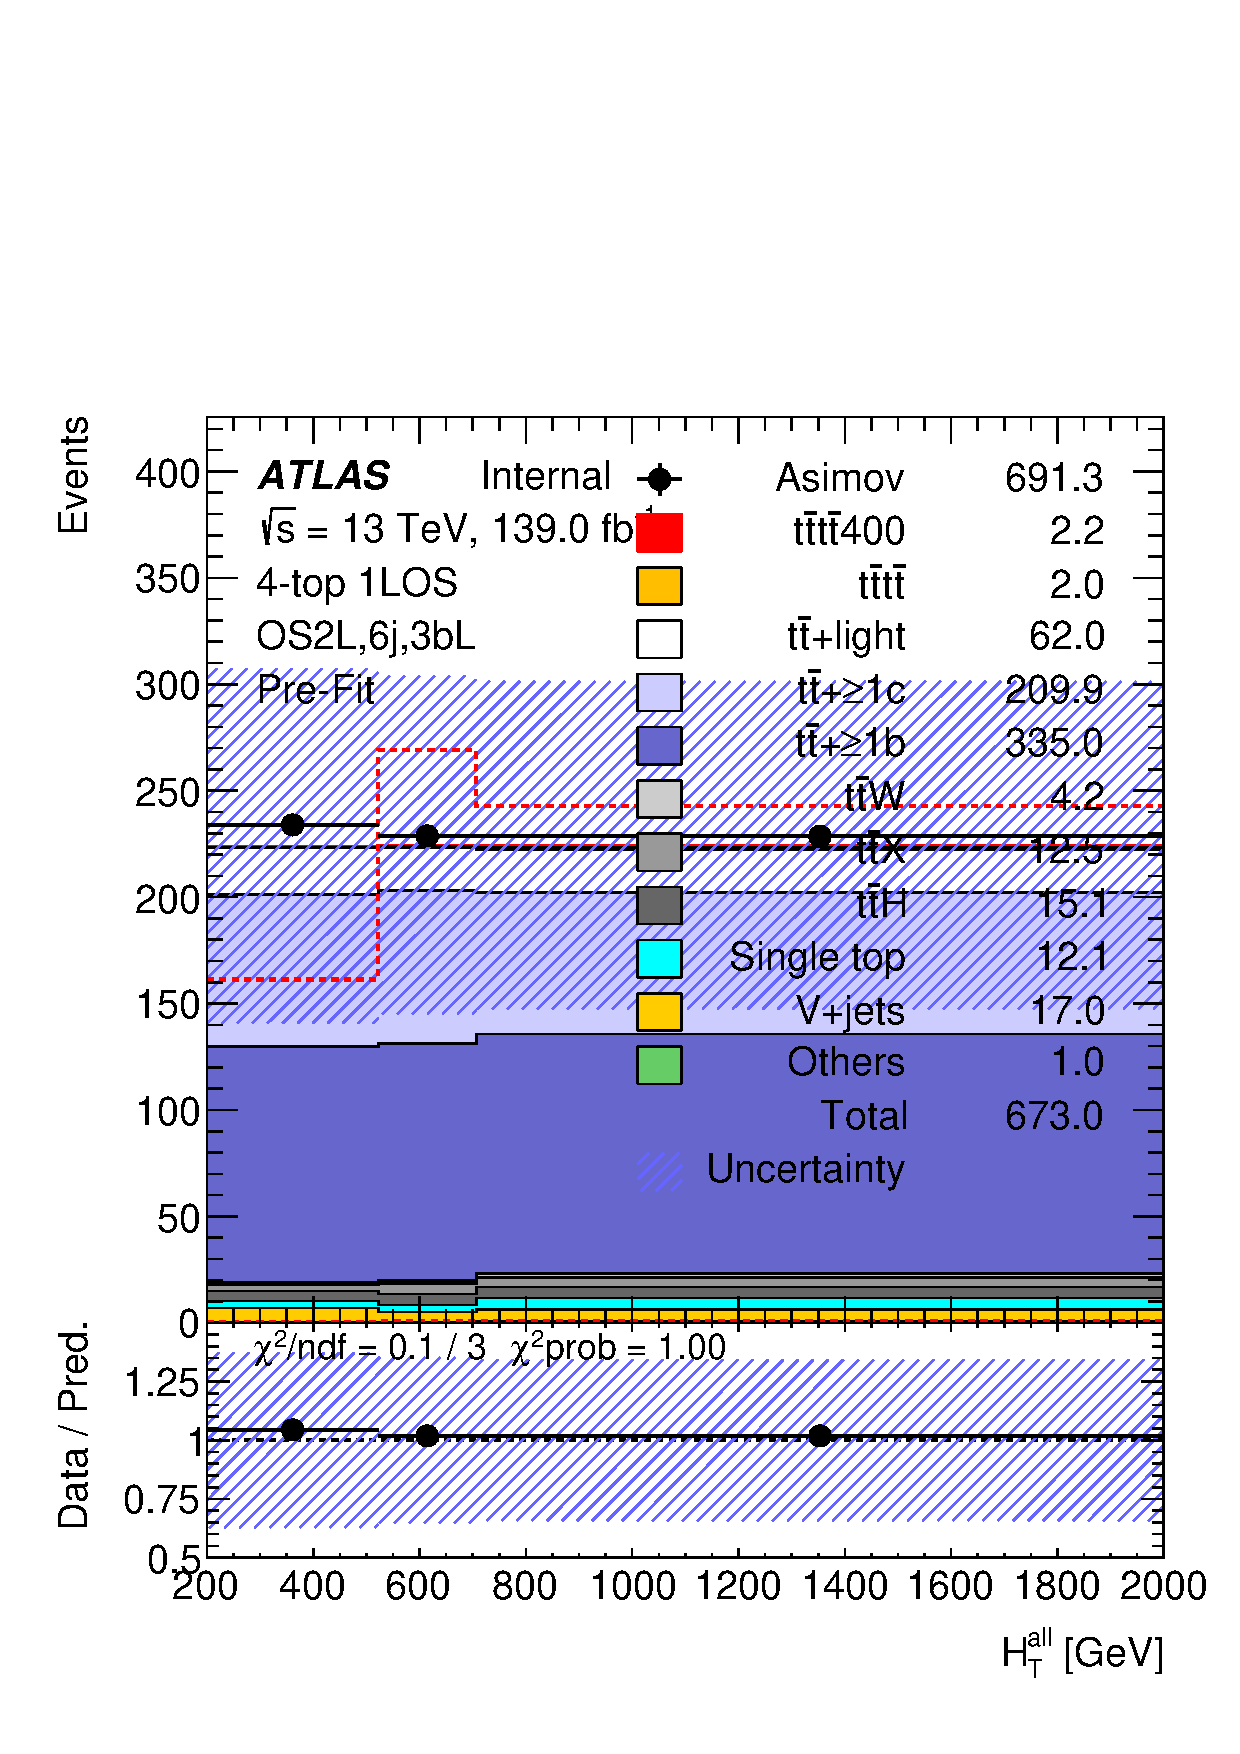
\includegraphics[width=0.31 \textwidth]{figures/4FS_studies/dataMC_4FSsyst_norew/os2l_6j3bL.pdf} &
        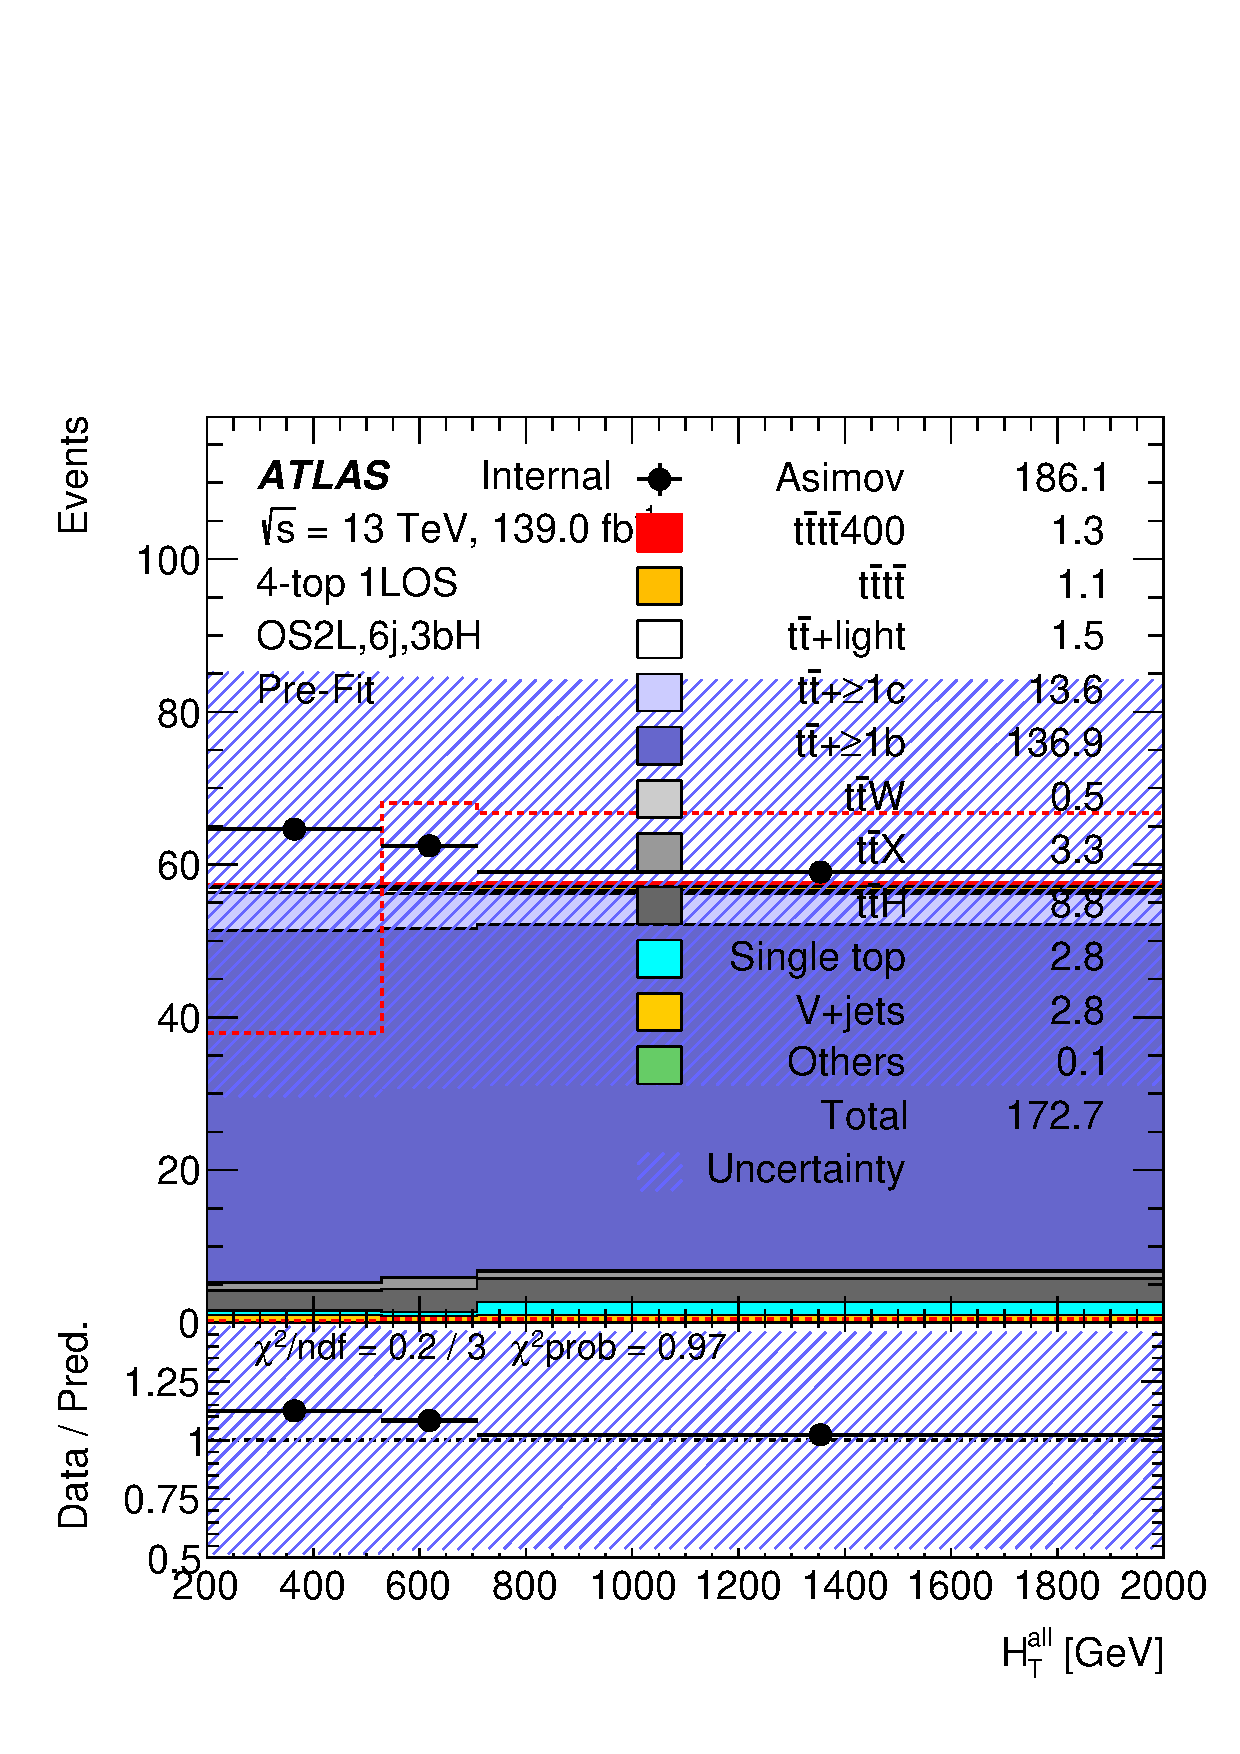
\includegraphics[width=0.31 \textwidth]{figures/4FS_studies/dataMC_4FSsyst_norew/os2l_6j3bH.pdf} &
        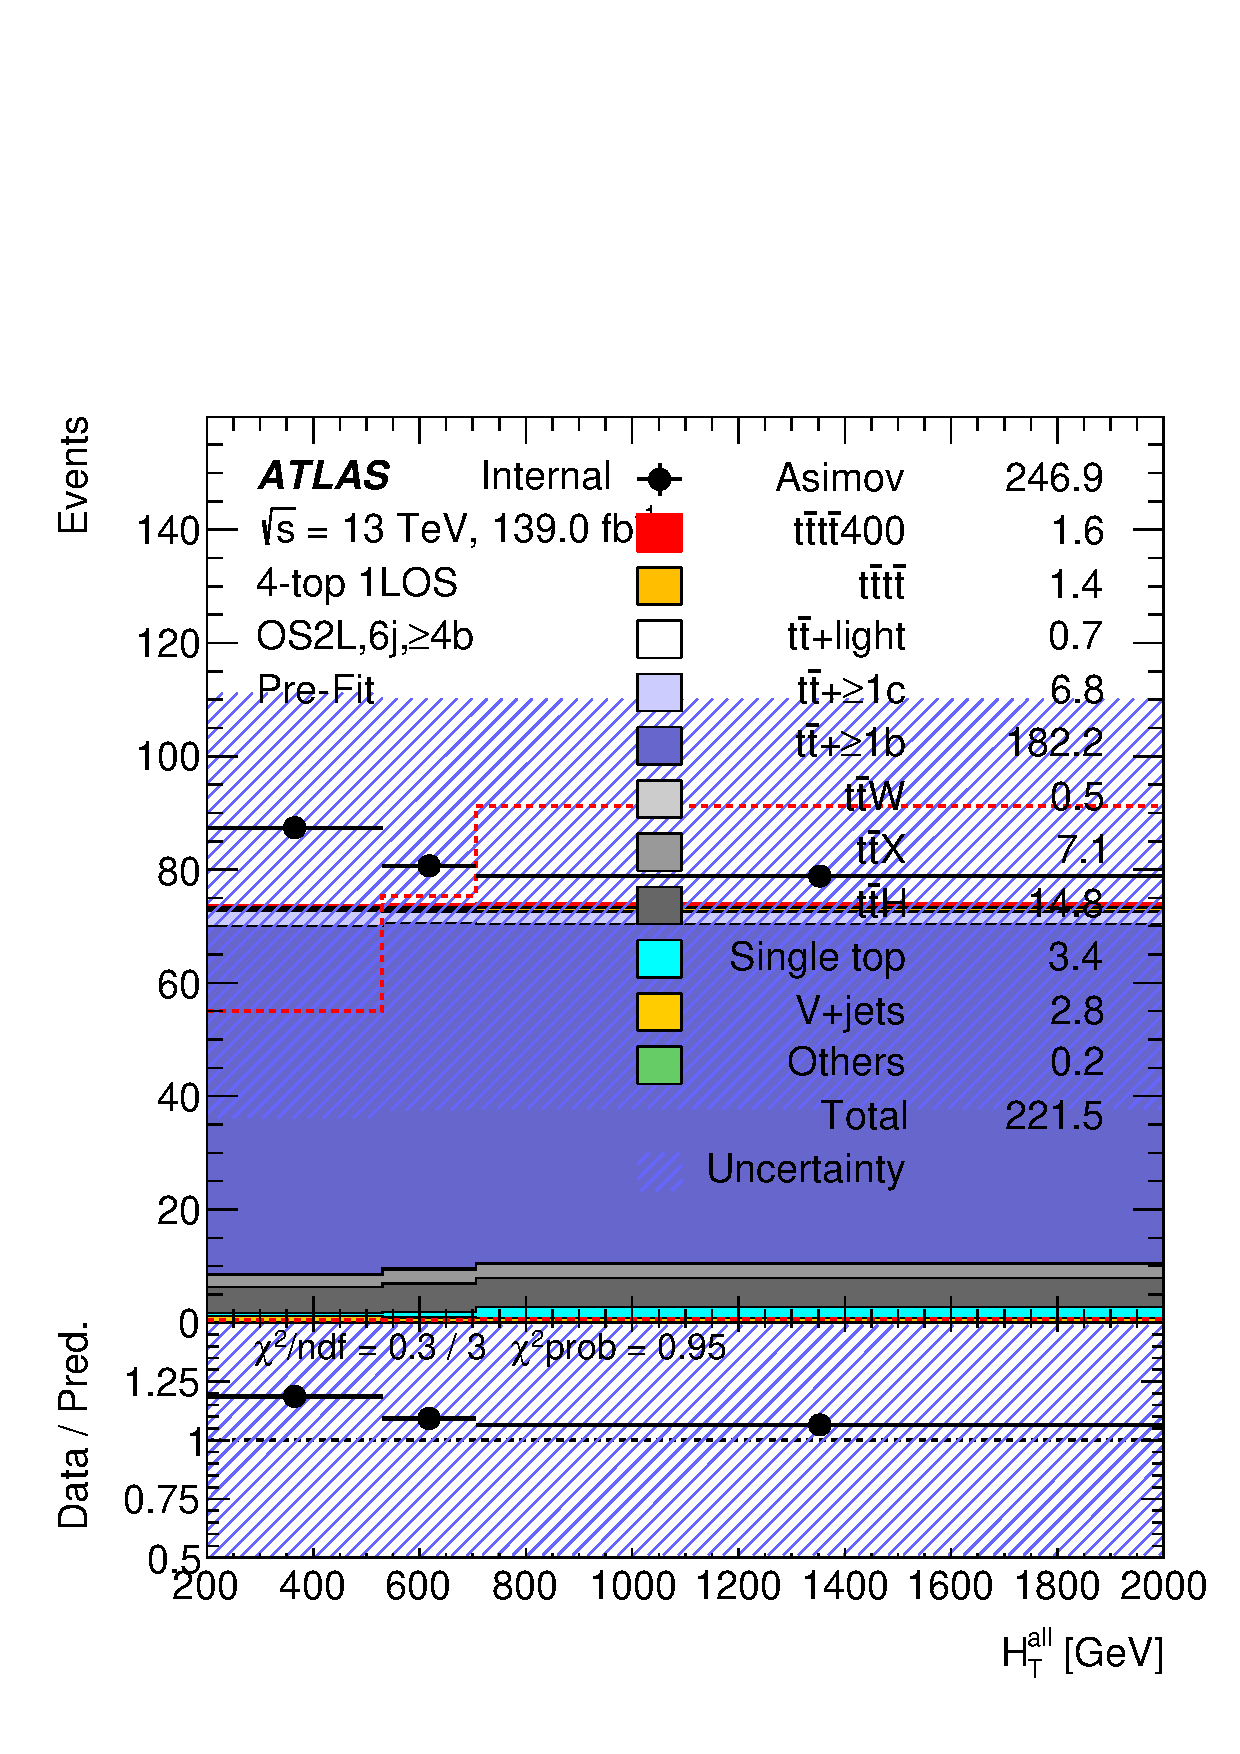
\includegraphics[width=0.31 \textwidth]{figures/4FS_studies/dataMC_4FSsyst_norew/os2l_6jge4b.pdf} \\

        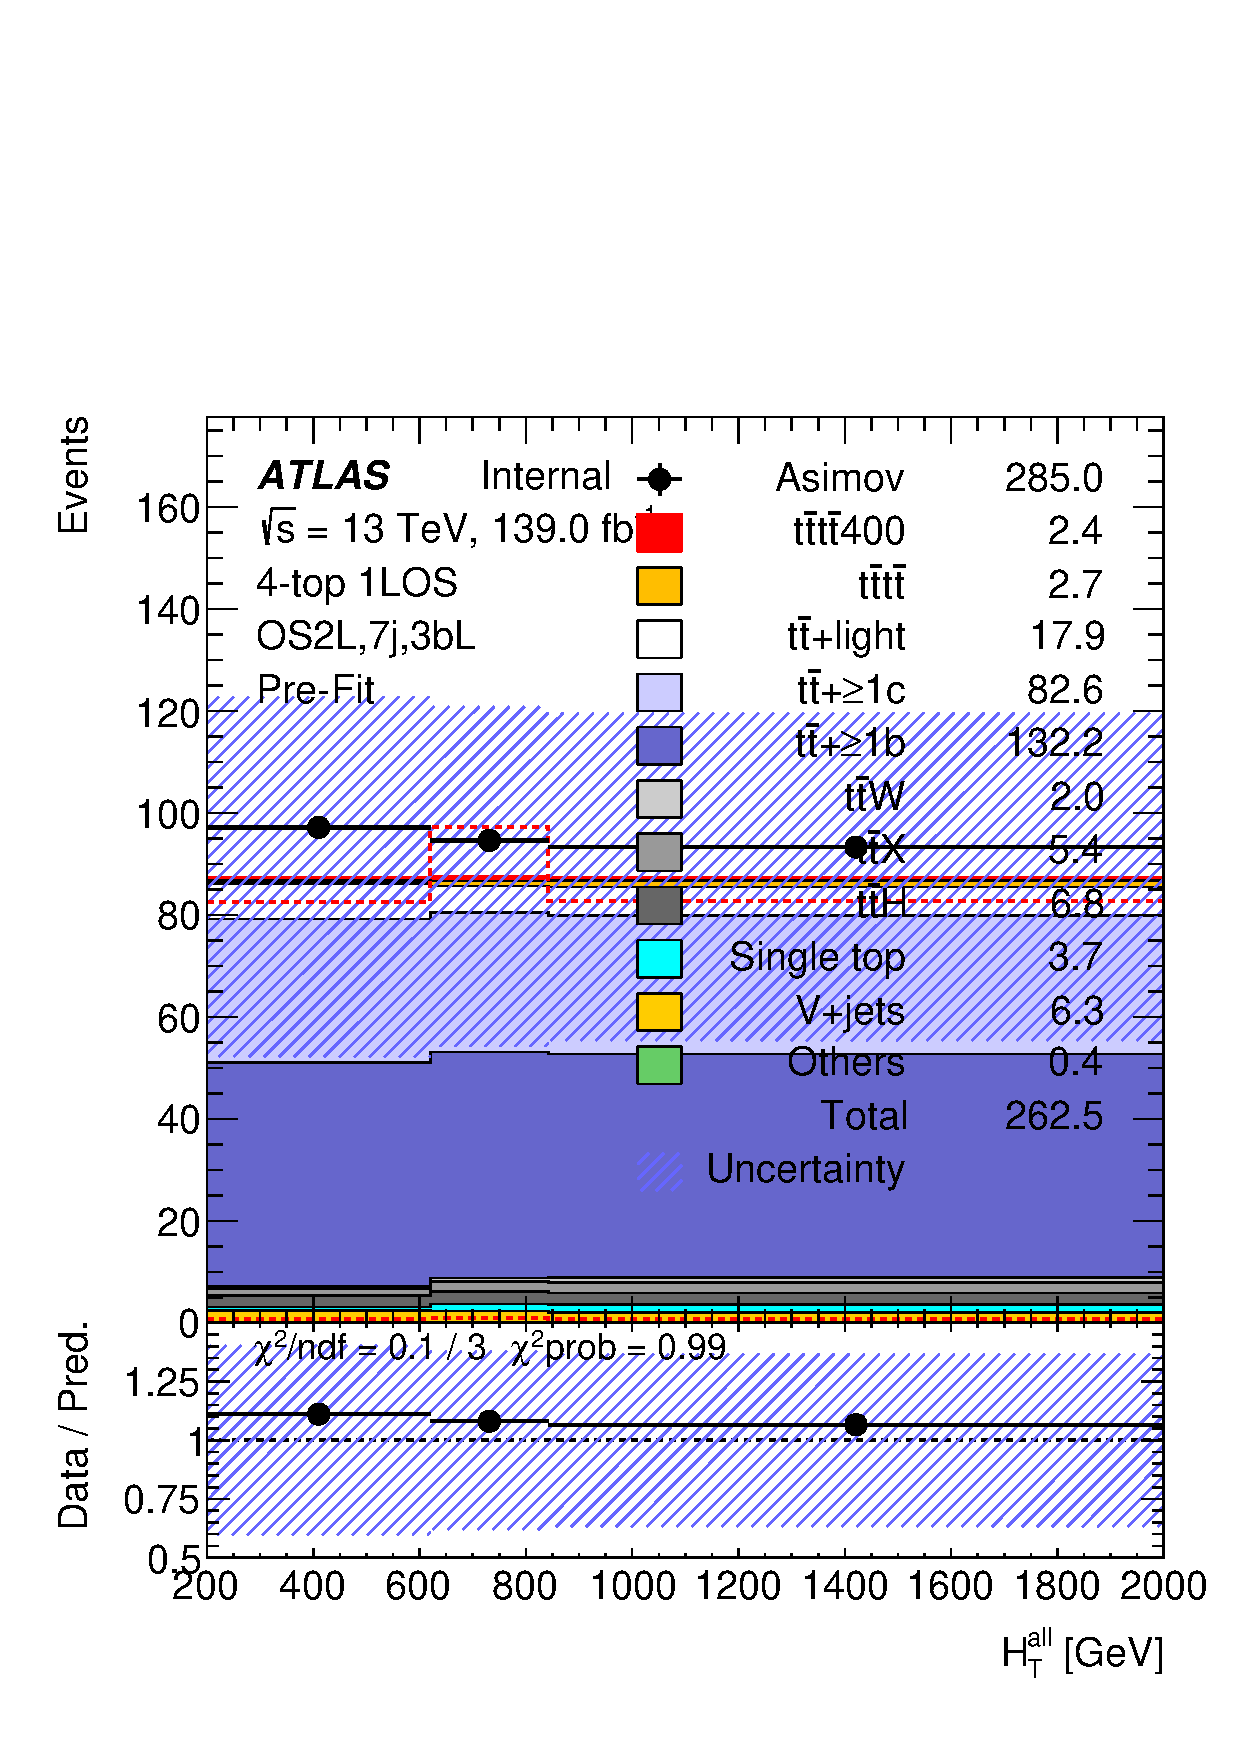
\includegraphics[width=0.31 \textwidth]{figures/4FS_studies/dataMC_4FSsyst_norew/os2l_7j3bL.pdf} &
        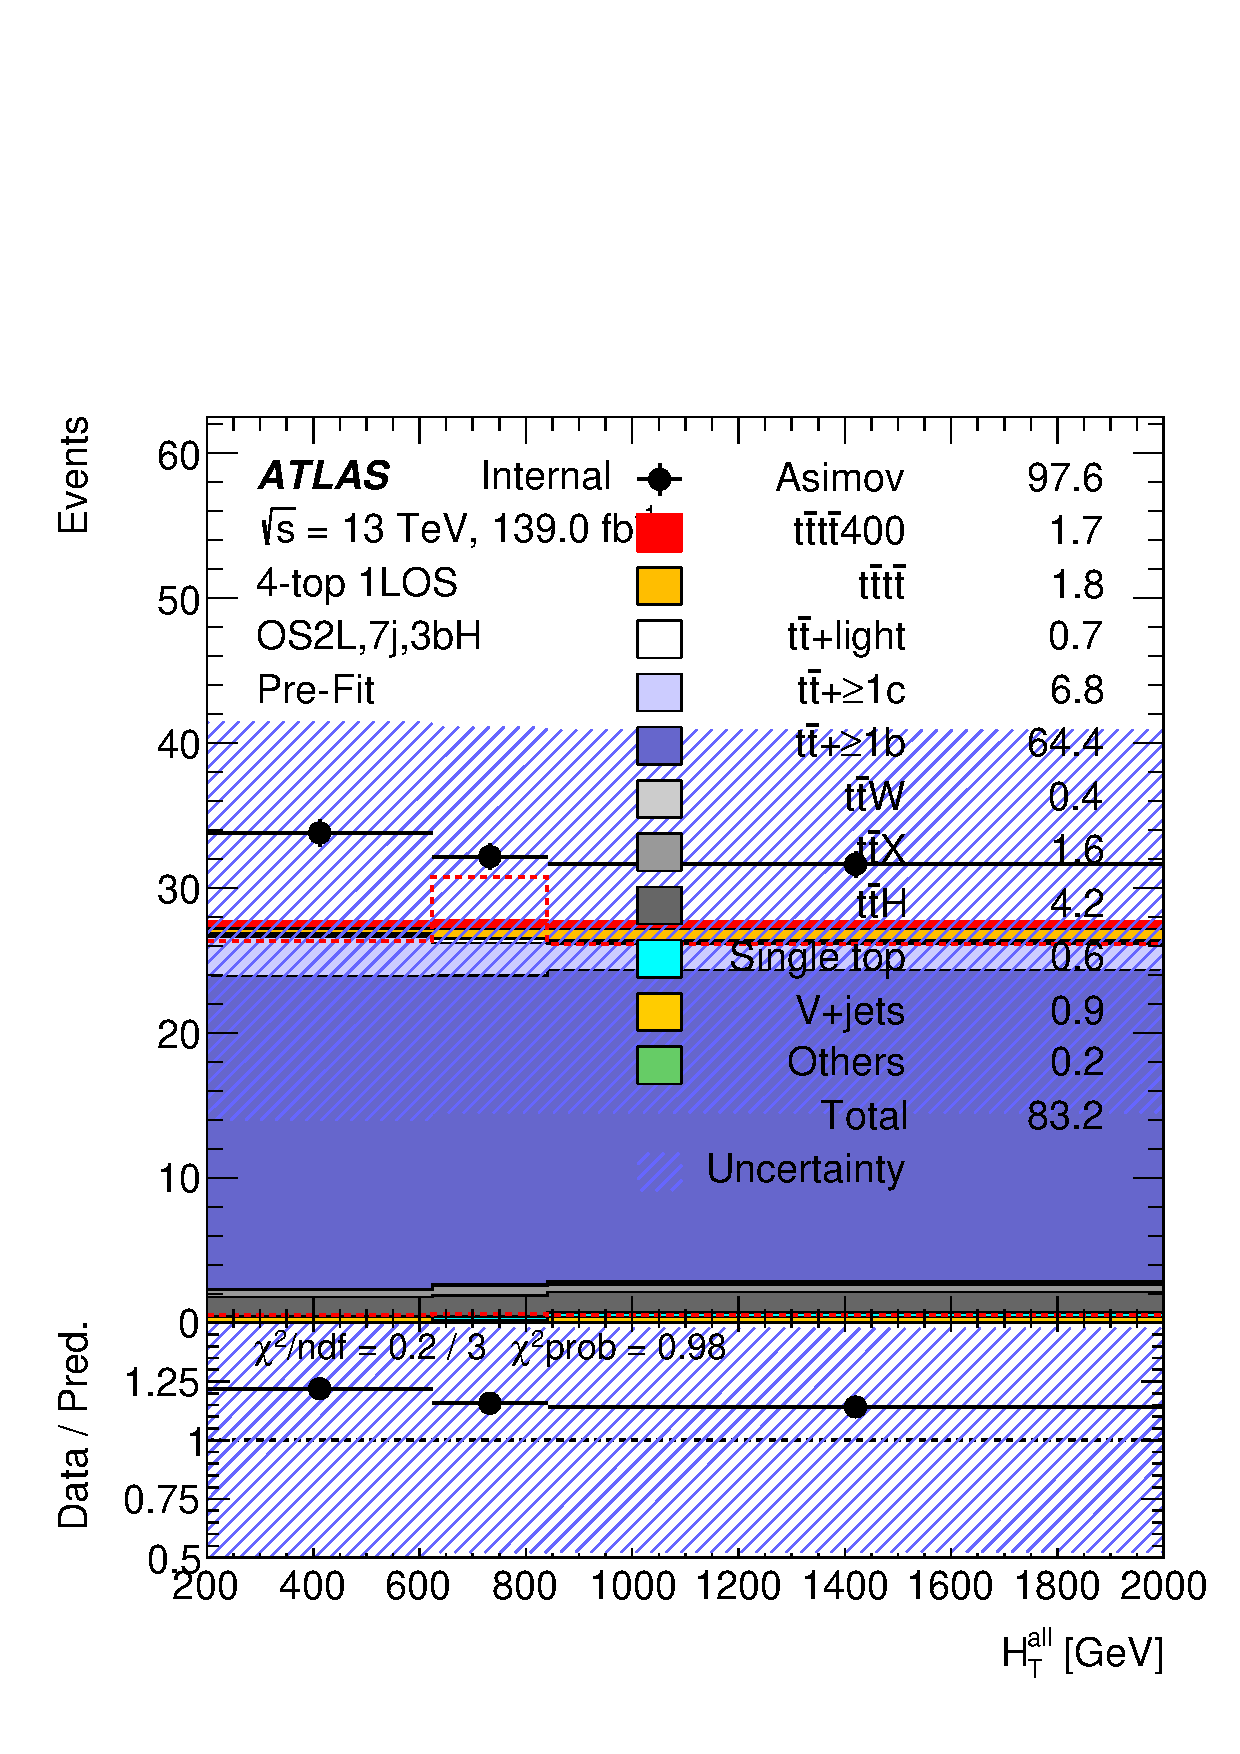
\includegraphics[width=0.31 \textwidth]{figures/4FS_studies/dataMC_4FSsyst_norew/os2l_7j3bH.pdf} &
        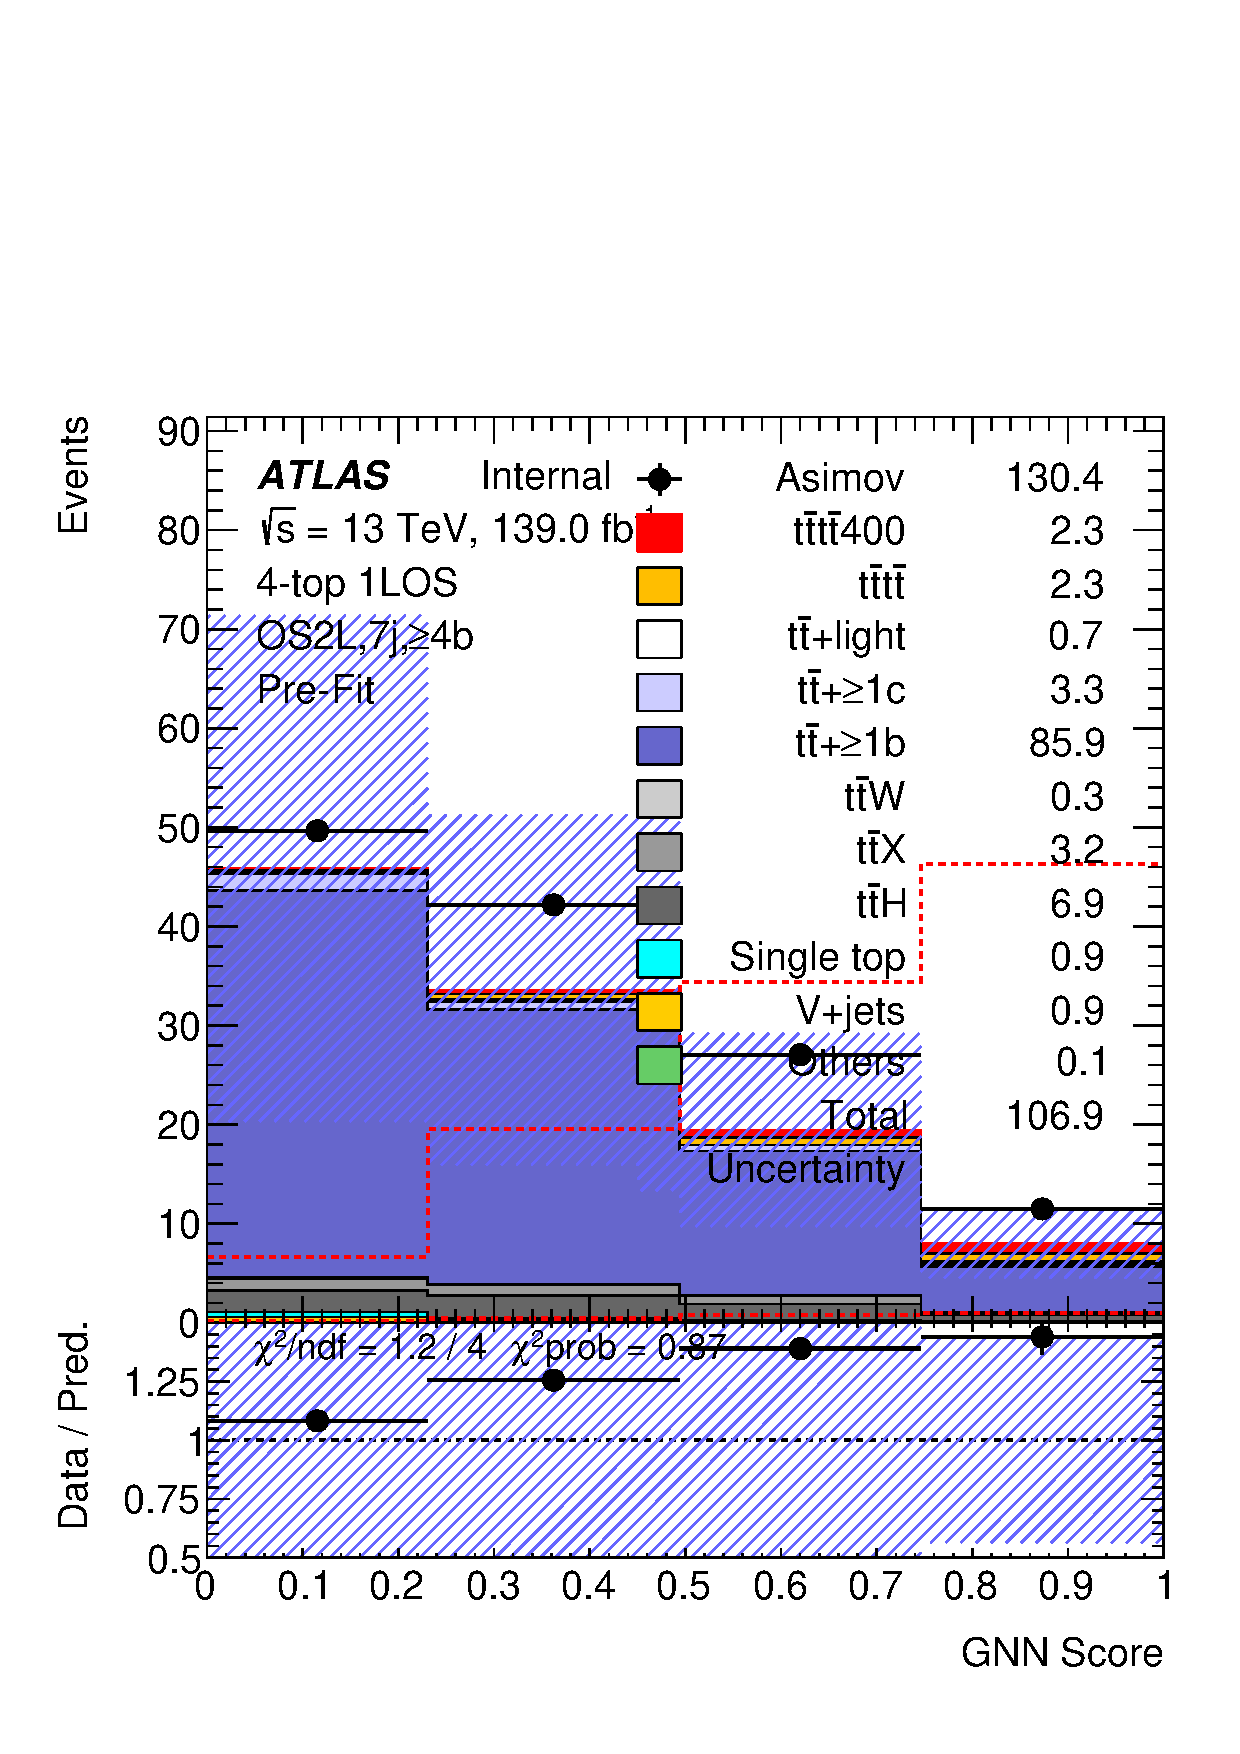
\includegraphics[width=0.31 \textwidth]{figures/4FS_studies/dataMC_4FSsyst_norew/os2l_7jge4b.pdf} \\

        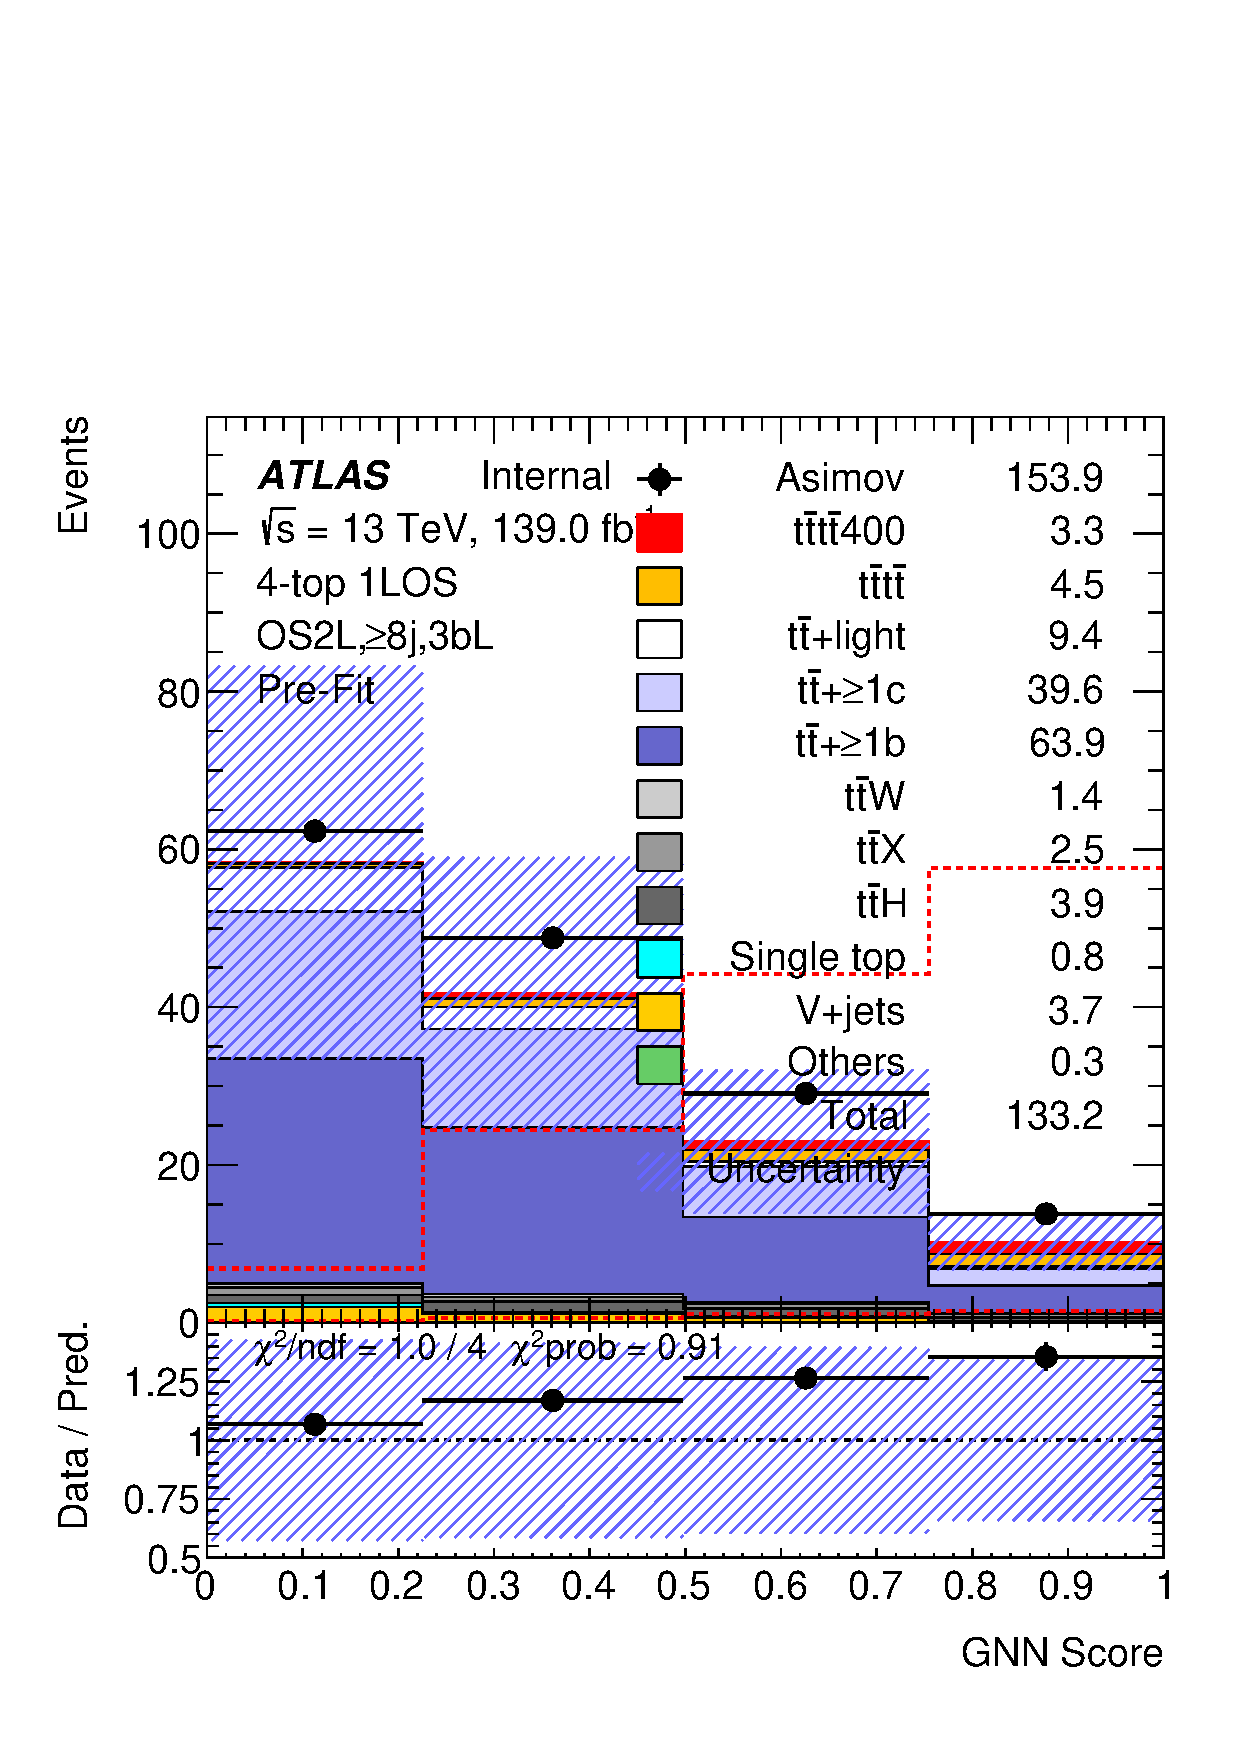
\includegraphics[width=0.31 \textwidth]{figures/4FS_studies/dataMC_4FSsyst_norew/os2l_ge8j3bL.pdf} &
        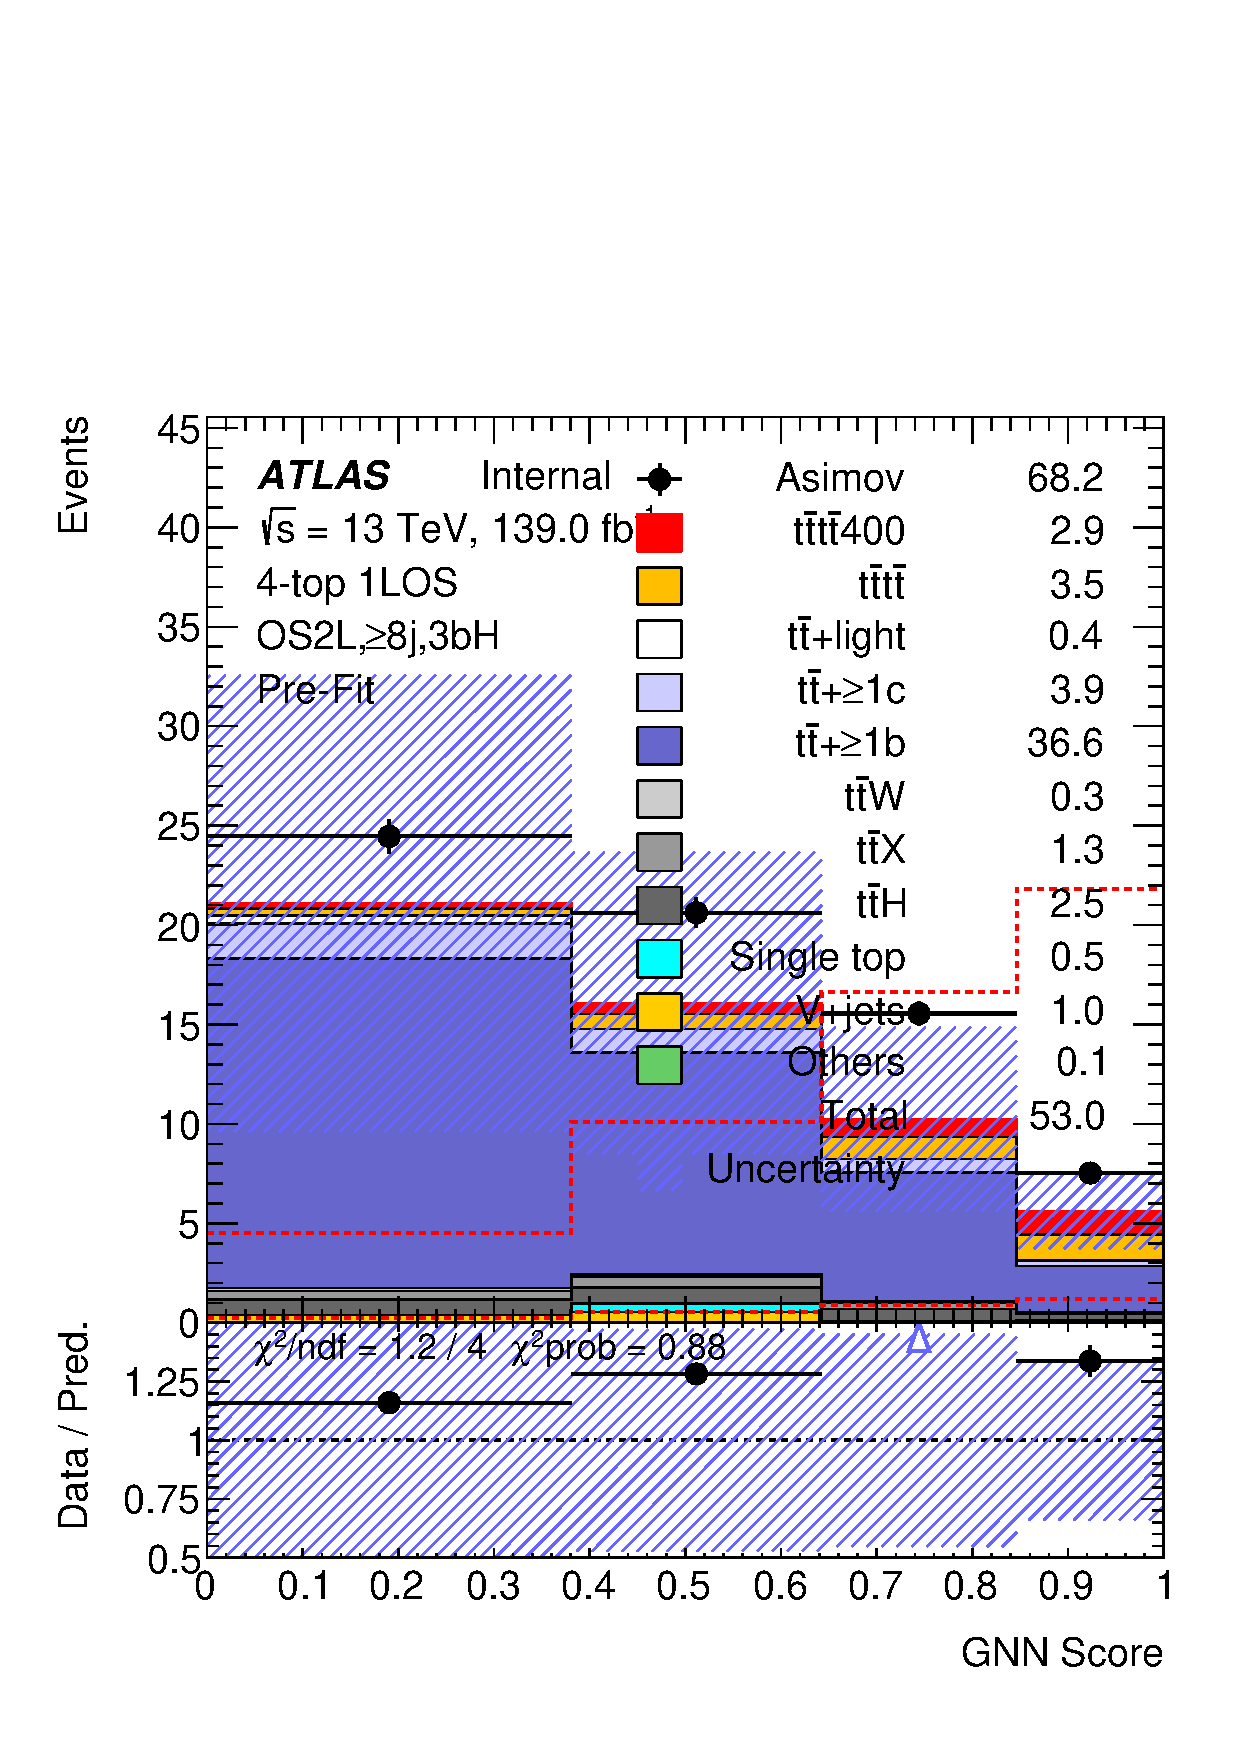
\includegraphics[width=0.31 \textwidth]{figures/4FS_studies/dataMC_4FSsyst_norew/os2l_ge8j3bH.pdf} &
        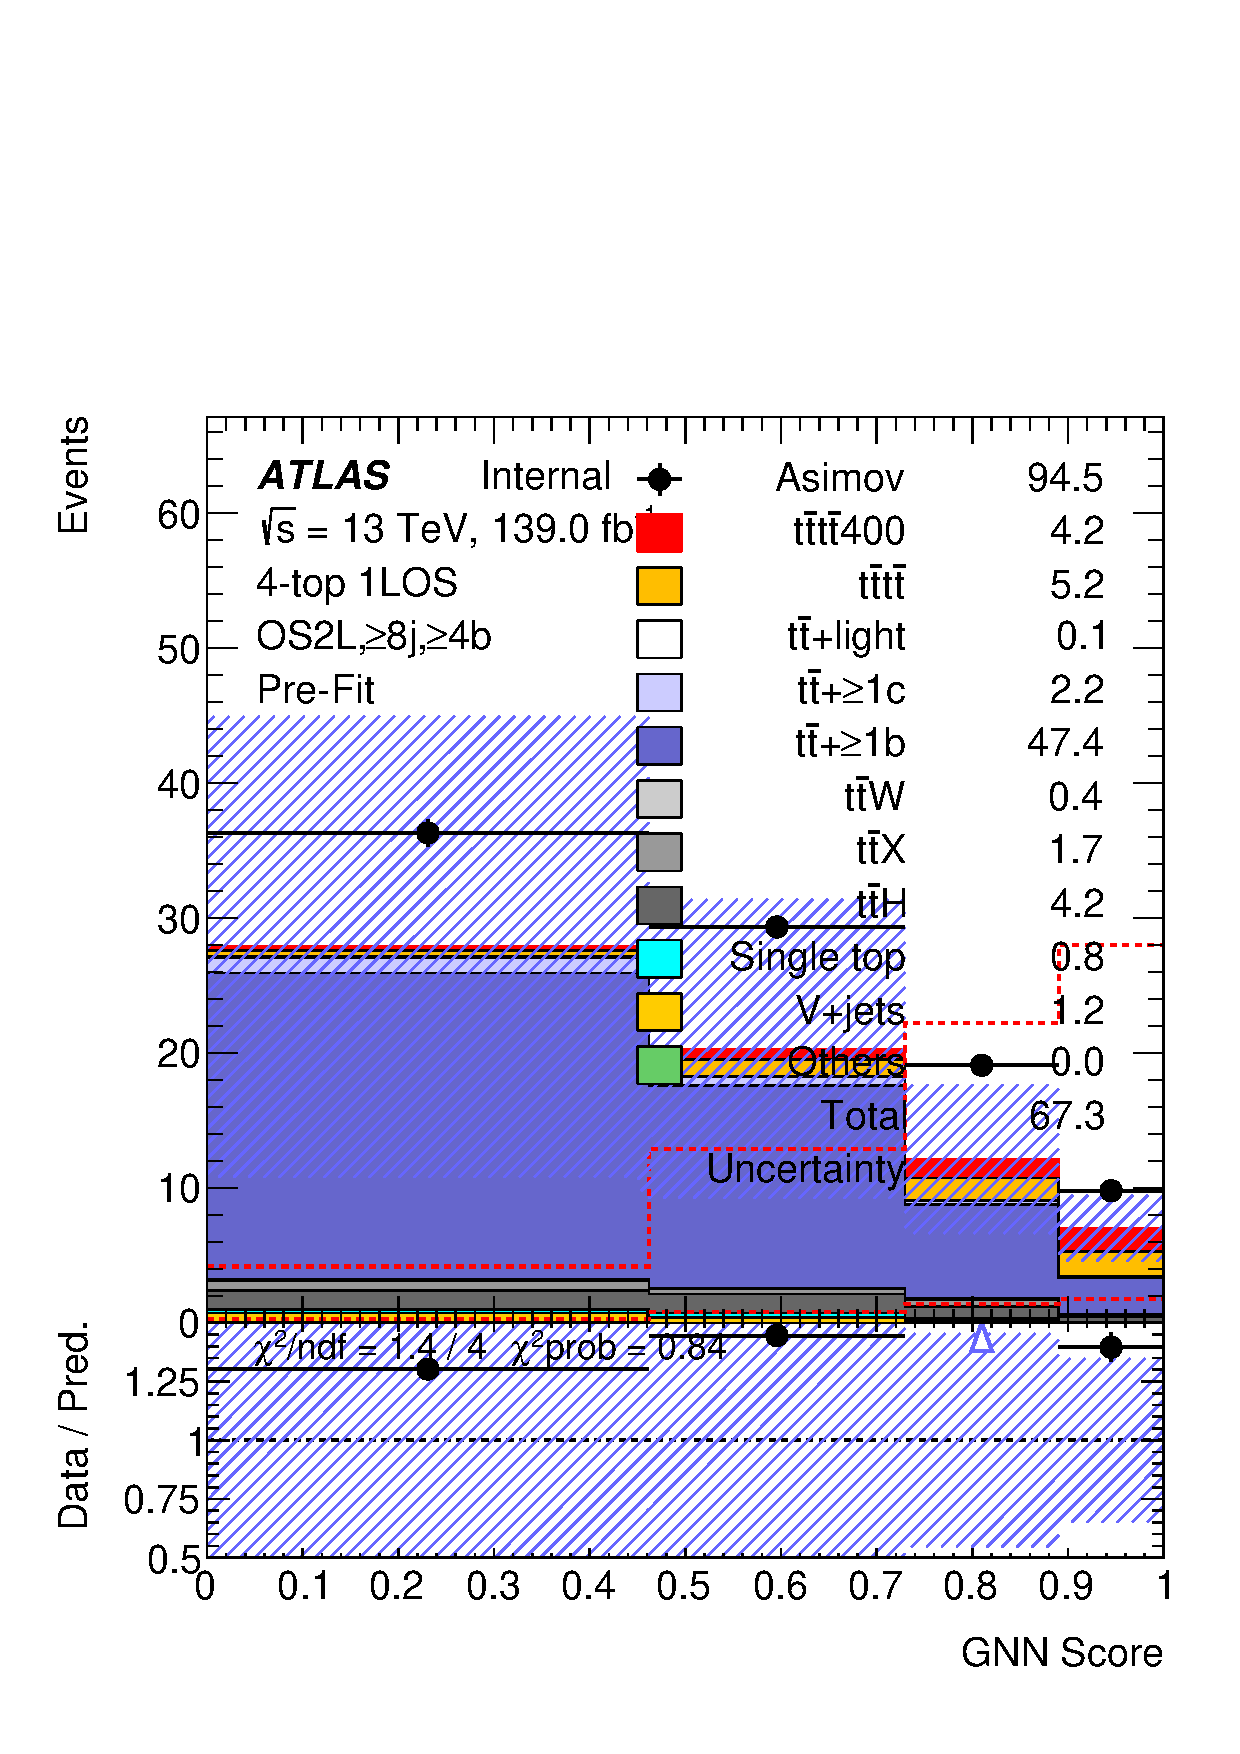
\includegraphics[width=0.31 \textwidth]{figures/4FS_studies/dataMC_4FSsyst_norew/os2l_ge8jge4b.pdf} \\
        \end{tabular}
        \caption{\label{fig:4FS_dataMC_4FSsyst_norew_2L_prefit}Pre-fit comparison of the 2LOS regions between samples with $t\bar{t}$ TTB samples produced with 5FS (MC) and $t\bar{t}$ TTB samples produced with 4FS (set as `pseudodata'). All systematics including 4FS systematics are incorporated in the uncertainty. The $t\bar{t}$ samples are not reweighted.}
\end{center}
\end{figure}

\begin{figure}[htbp!]
        \begin{center} \setlength{\tabcolsep}{2.5pt}\footnotesize
        \begin{tabular}{cccc}
        
\includegraphics[width=0.23 \textwidth]{figures/4FS_studies/dataMC_syst_rew/ljets_8j3bL_postFit.pdf} &
        
\includegraphics[width=0.23 \textwidth]{figures/4FS_studies/dataMC_syst_rew/ljets_8j3bH_postFit.pdf} &
        
\includegraphics[width=0.23 \textwidth]{figures/4FS_studies/dataMC_syst_rew/ljets_8j4b_postFit.pdf} &
        
\includegraphics[width=0.23 \textwidth]{figures/4FS_studies/dataMC_syst_rew/ljets_8jge5b_postFit.pdf}\\

        
\includegraphics[width=0.23 \textwidth]{figures/4FS_studies/dataMC_syst_rew/ljets_9j3bL_postFit.pdf} &
        
\includegraphics[width=0.23 \textwidth]{figures/4FS_studies/dataMC_syst_rew/ljets_9j3bH_postFit.pdf} &
        
\includegraphics[width=0.23 \textwidth]{figures/4FS_studies/dataMC_syst_rew/ljets_9j4b_postFit.pdf} &
        
\includegraphics[width=0.23 \textwidth]{figures/4FS_studies/dataMC_syst_rew/ljets_9jge5b_postFit.pdf} \\

        
\includegraphics[width=0.23 \textwidth]{figures/4FS_studies/dataMC_syst_rew/ljets_ge10j3bL_postFit.pdf} &
        
\includegraphics[width=0.23 \textwidth]{figures/4FS_studies/dataMC_syst_rew/ljets_ge10j3bH_postFit.pdf} &
        
\includegraphics[width=0.23 \textwidth]{figures/4FS_studies/dataMC_syst_rew/ljets_ge10j4b_postFit.pdf} &
        
\includegraphics[width=0.23 \textwidth]{figures/4FS_studies/dataMC_syst_rew/ljets_ge10jge5b_postFit.pdf} \\
        \end{tabular}
        \caption{\label{fig:4FS_dataMC_syst_rew_1L_postfit}Post-fit comparison of the 1L regions between samples with $t\bar{t}$ TTB samples produced with 5FS (MC) and $t\bar{t}$ TTB samples produced with 4FS (set as `pseudodata'). All systematics except 4FS systematics are included. The $t\bar{t}$ samples are reweighted.}
\end{center}
\end{figure}

\begin{figure}[htbp!]
        \begin{center} \setlength{\tabcolsep}{2.5pt}\footnotesize
        \begin{tabular}{ccc}
        
\includegraphics[width=0.31 \textwidth]{figures/4FS_studies/dataMC_syst_rew/os2l_6j3bL_postFit.pdf} &
        
\includegraphics[width=0.31 \textwidth]{figures/4FS_studies/dataMC_syst_rew/os2l_6j3bH_postFit.pdf} &
        
\includegraphics[width=0.31 \textwidth]{figures/4FS_studies/dataMC_syst_rew/os2l_6jge4b_postFit.pdf} \\

        
\includegraphics[width=0.31 \textwidth]{figures/4FS_studies/dataMC_syst_rew/os2l_7j3bL_postFit.pdf} &
        
\includegraphics[width=0.31 \textwidth]{figures/4FS_studies/dataMC_syst_rew/os2l_7j3bH_postFit.pdf} &
        
\includegraphics[width=0.31 \textwidth]{figures/4FS_studies/dataMC_syst_rew/os2l_7jge4b_postFit.pdf} \\

        
\includegraphics[width=0.31 \textwidth]{figures/4FS_studies/dataMC_syst_rew/os2l_ge8j3bL_postFit.pdf} &
        
\includegraphics[width=0.31 \textwidth]{figures/4FS_studies/dataMC_syst_rew/os2l_ge8j3bH_postFit.pdf} &
        
\includegraphics[width=0.31 \textwidth]{figures/4FS_studies/dataMC_syst_rew/os2l_ge8jge4b_postFit.pdf} \\
        \end{tabular}
        \caption{\label{fig:4FS_dataMC_syst_rew_2L_postfit}Post-fit comparison of the 2LOS regions between samples with $t\bar{t}$ TTB samples produced with 5FS (MC) and $t\bar{t}$ TTB samples produced with 4FS (set as `pseudodata'). All systematics except 4FS systematics are included. The $t\bar{t}$ samples are reweighted.}
\end{center}
\end{figure}


\begin{figure}[htbp!]
        \begin{center} \setlength{\tabcolsep}{2.5pt}\footnotesize
        \begin{tabular}{cccc}
        
\includegraphics[width=0.23 \textwidth]{figures/4FS_studies/dataMC_4FSsyst_rew/ljets_8j3bL_postFit.pdf} &
        
\includegraphics[width=0.23 \textwidth]{figures/4FS_studies/dataMC_4FSsyst_rew/ljets_8j3bH_postFit.pdf} &
        
\includegraphics[width=0.23 \textwidth]{figures/4FS_studies/dataMC_4FSsyst_rew/ljets_8j4b_postFit.pdf} &
        
\includegraphics[width=0.23 \textwidth]{figures/4FS_studies/dataMC_4FSsyst_rew/ljets_8jge5b_postFit.pdf}\\

        
\includegraphics[width=0.23 \textwidth]{figures/4FS_studies/dataMC_4FSsyst_rew/ljets_9j3bL_postFit.pdf} &
        
\includegraphics[width=0.23 \textwidth]{figures/4FS_studies/dataMC_4FSsyst_rew/ljets_9j3bH_postFit.pdf} &
        
\includegraphics[width=0.23 \textwidth]{figures/4FS_studies/dataMC_4FSsyst_rew/ljets_9j4b_postFit.pdf} &
        
\includegraphics[width=0.23 \textwidth]{figures/4FS_studies/dataMC_4FSsyst_rew/ljets_9jge5b_postFit.pdf} \\

        
\includegraphics[width=0.23 \textwidth]{figures/4FS_studies/dataMC_4FSsyst_rew/ljets_ge10j3bL_postFit.pdf} &
        
\includegraphics[width=0.23 \textwidth]{figures/4FS_studies/dataMC_4FSsyst_rew/ljets_ge10j3bH_postFit.pdf} &
        
\includegraphics[width=0.23 \textwidth]{figures/4FS_studies/dataMC_4FSsyst_rew/ljets_ge10j4b_postFit.pdf} &
        
\includegraphics[width=0.23 \textwidth]{figures/4FS_studies/dataMC_4FSsyst_rew/ljets_ge10jge5b_postFit.pdf} \\
        \end{tabular}
        \caption{\label{fig:4FS_dataMC_4FSsyst_rew_1L_postfit}Post-fit comparison of the 1L regions between samples with $t\bar{t}$ TTB samples produced with 5FS (MC) and $t\bar{t}$ TTB samples produced with 4FS (set as `pseudodata'). All systematics including 4FS systematics are incorporated in the uncertainty. The $t\bar{t}$ samples are reweighted.}
\end{center}
\end{figure}

\begin{figure}[htbp!]
        \begin{center} \setlength{\tabcolsep}{2.5pt}\footnotesize
        \begin{tabular}{ccc}
        
\includegraphics[width=0.31 \textwidth]{figures/4FS_studies/dataMC_4FSsyst_rew/os2l_6j3bL_postFit.pdf} &
        
\includegraphics[width=0.31 \textwidth]{figures/4FS_studies/dataMC_4FSsyst_rew/os2l_6j3bH_postFit.pdf} &
        
\includegraphics[width=0.31 \textwidth]{figures/4FS_studies/dataMC_4FSsyst_rew/os2l_6jge4b_postFit.pdf} \\

        
\includegraphics[width=0.31 \textwidth]{figures/4FS_studies/dataMC_4FSsyst_rew/os2l_7j3bL_postFit.pdf} &
        
\includegraphics[width=0.31 \textwidth]{figures/4FS_studies/dataMC_4FSsyst_rew/os2l_7j3bH_postFit.pdf} &
        
\includegraphics[width=0.31 \textwidth]{figures/4FS_studies/dataMC_4FSsyst_rew/os2l_7jge4b_postFit.pdf} \\

        
\includegraphics[width=0.31 \textwidth]{figures/4FS_studies/dataMC_4FSsyst_rew/os2l_ge8j3bL_postFit.pdf} &
        
\includegraphics[width=0.31 \textwidth]{figures/4FS_studies/dataMC_4FSsyst_rew/os2l_ge8j3bH_postFit.pdf} &
        
\includegraphics[width=0.31 \textwidth]{figures/4FS_studies/dataMC_4FSsyst_rew/os2l_ge8jge4b_postFit.pdf} \\
        \end{tabular}
        \caption{\label{fig:4FS_dataMC_4FSsyst_rew_2L_postfit}Post-fit comparison of the 2LOS regions between samples with $t\bar{t}$ TTB samples produced with 5FS (MC) and $t\bar{t}$ TTB samples produced with 4FS (set as `pseudodata'). All systematics including 4FS systematics are incorporated in the uncertainty. The $t\bar{t}$ samples are reweighted.}
\end{center}
\end{figure}

\begin{figure}[htbp!]
        \begin{center} \setlength{\tabcolsep}{2.5pt}\footnotesize
        \begin{tabular}{cccc}
        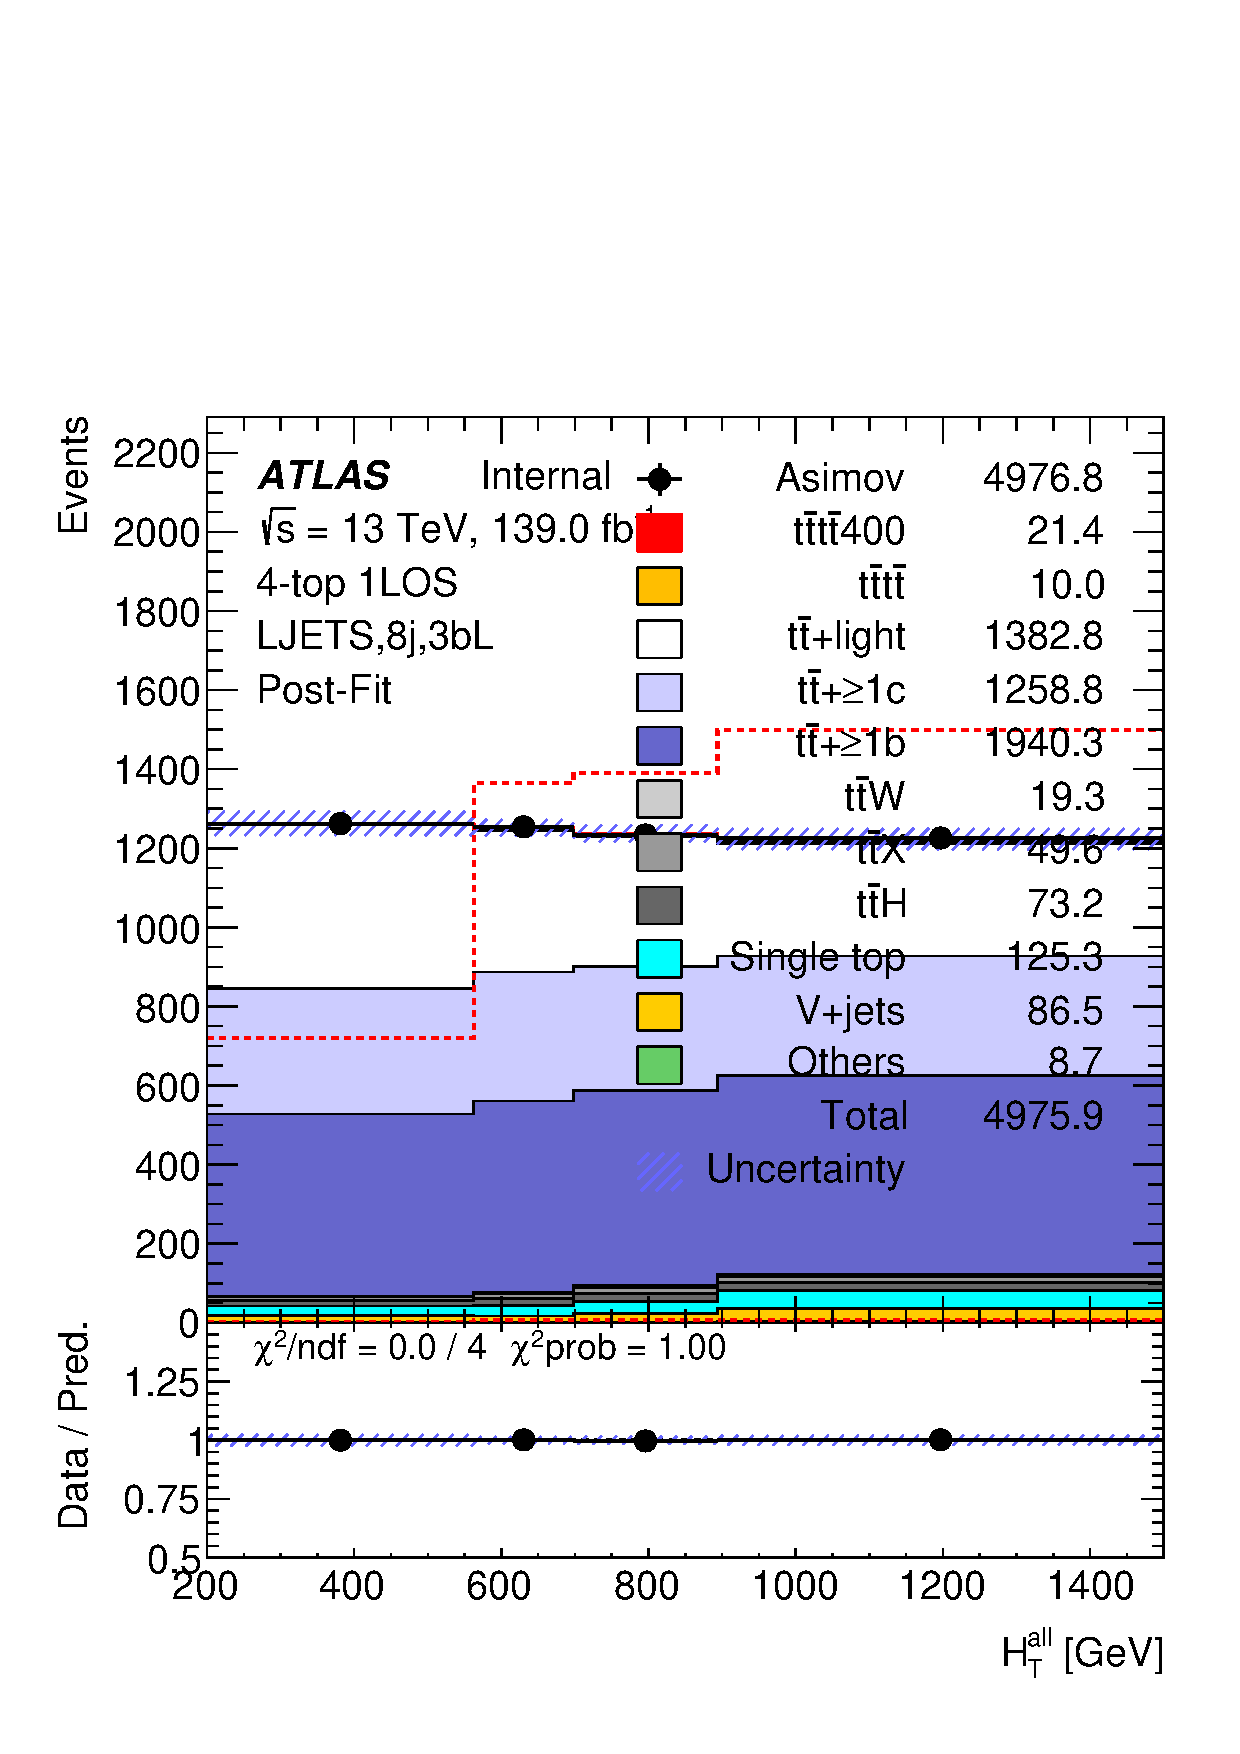
\includegraphics[width=0.23 \textwidth]{figures/4FS_studies/dataMC_4FSsyst_norew/ljets_8j3bL_postFit.pdf} &
        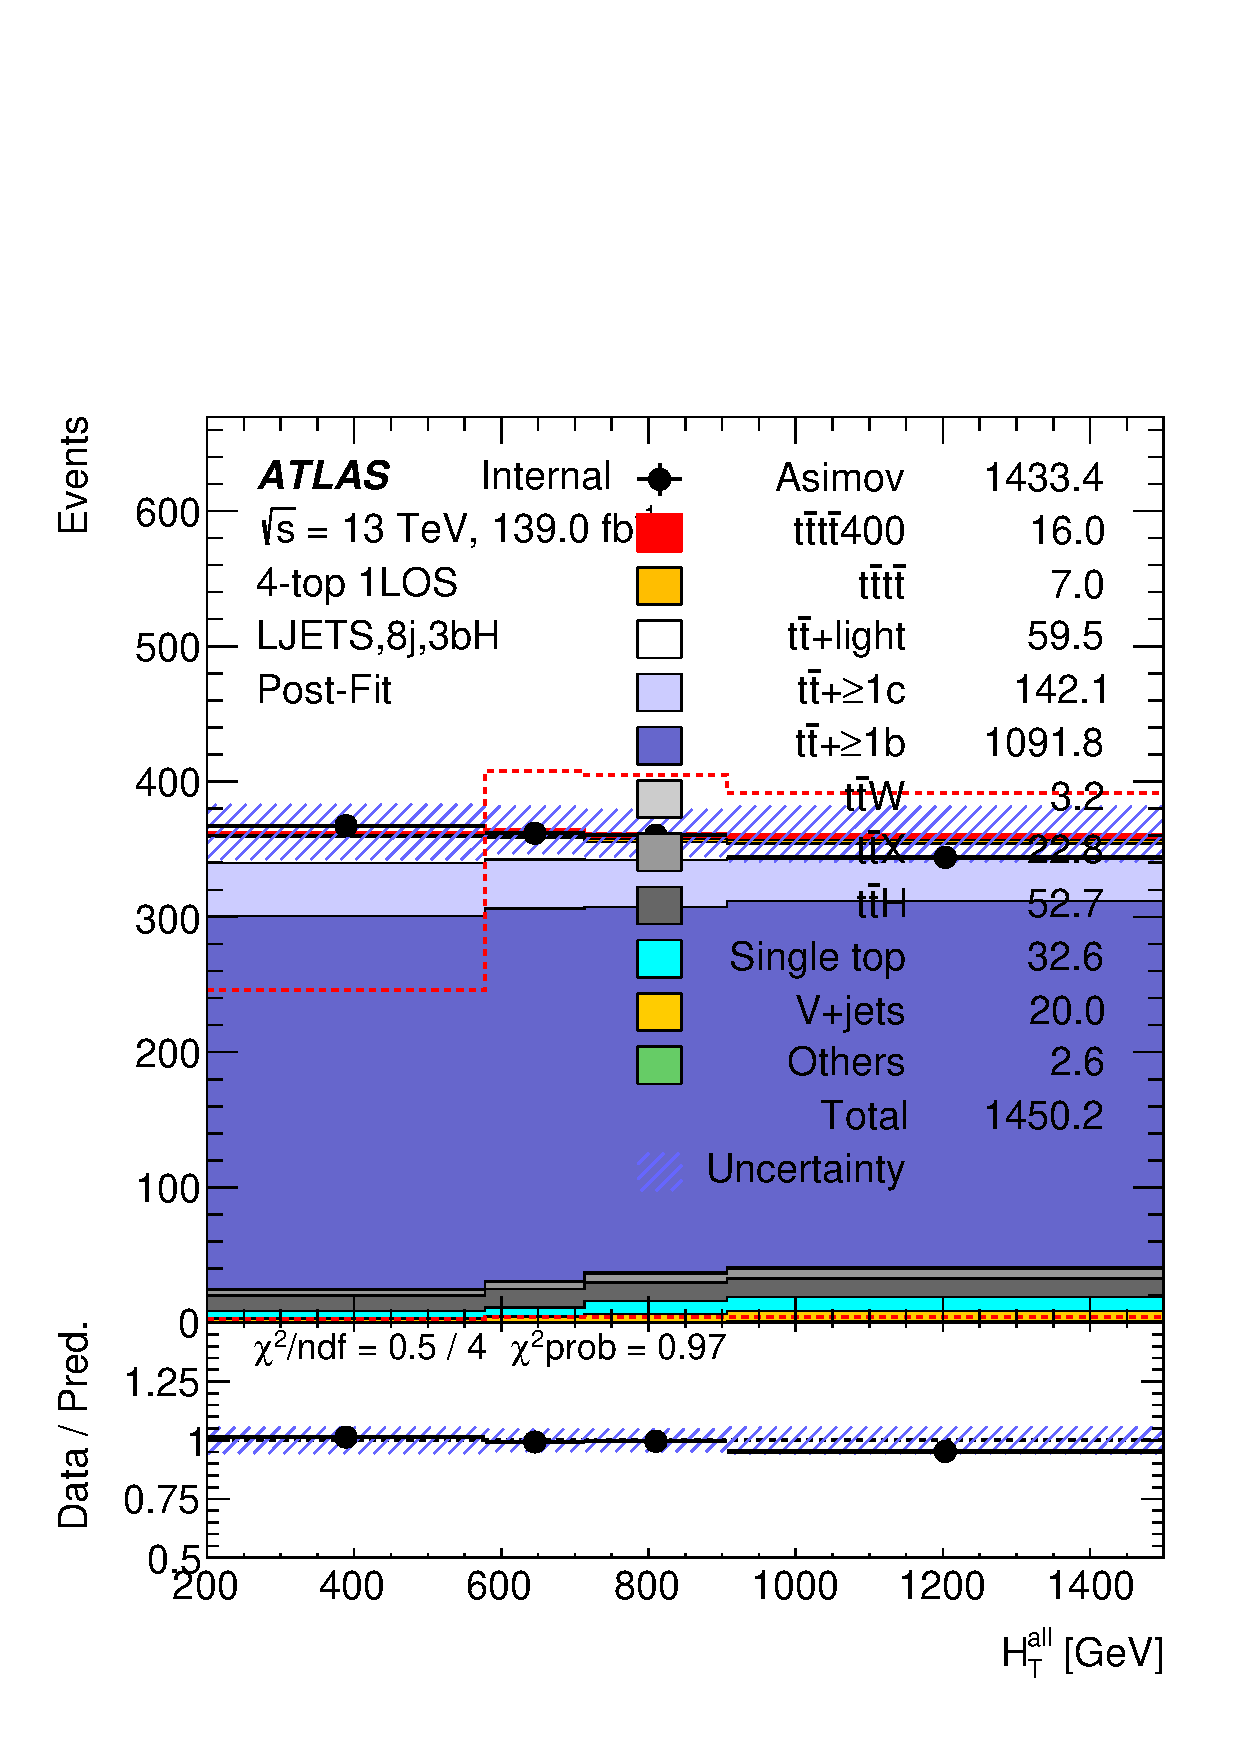
\includegraphics[width=0.23 \textwidth]{figures/4FS_studies/dataMC_4FSsyst_norew/ljets_8j3bH_postFit.pdf} &
        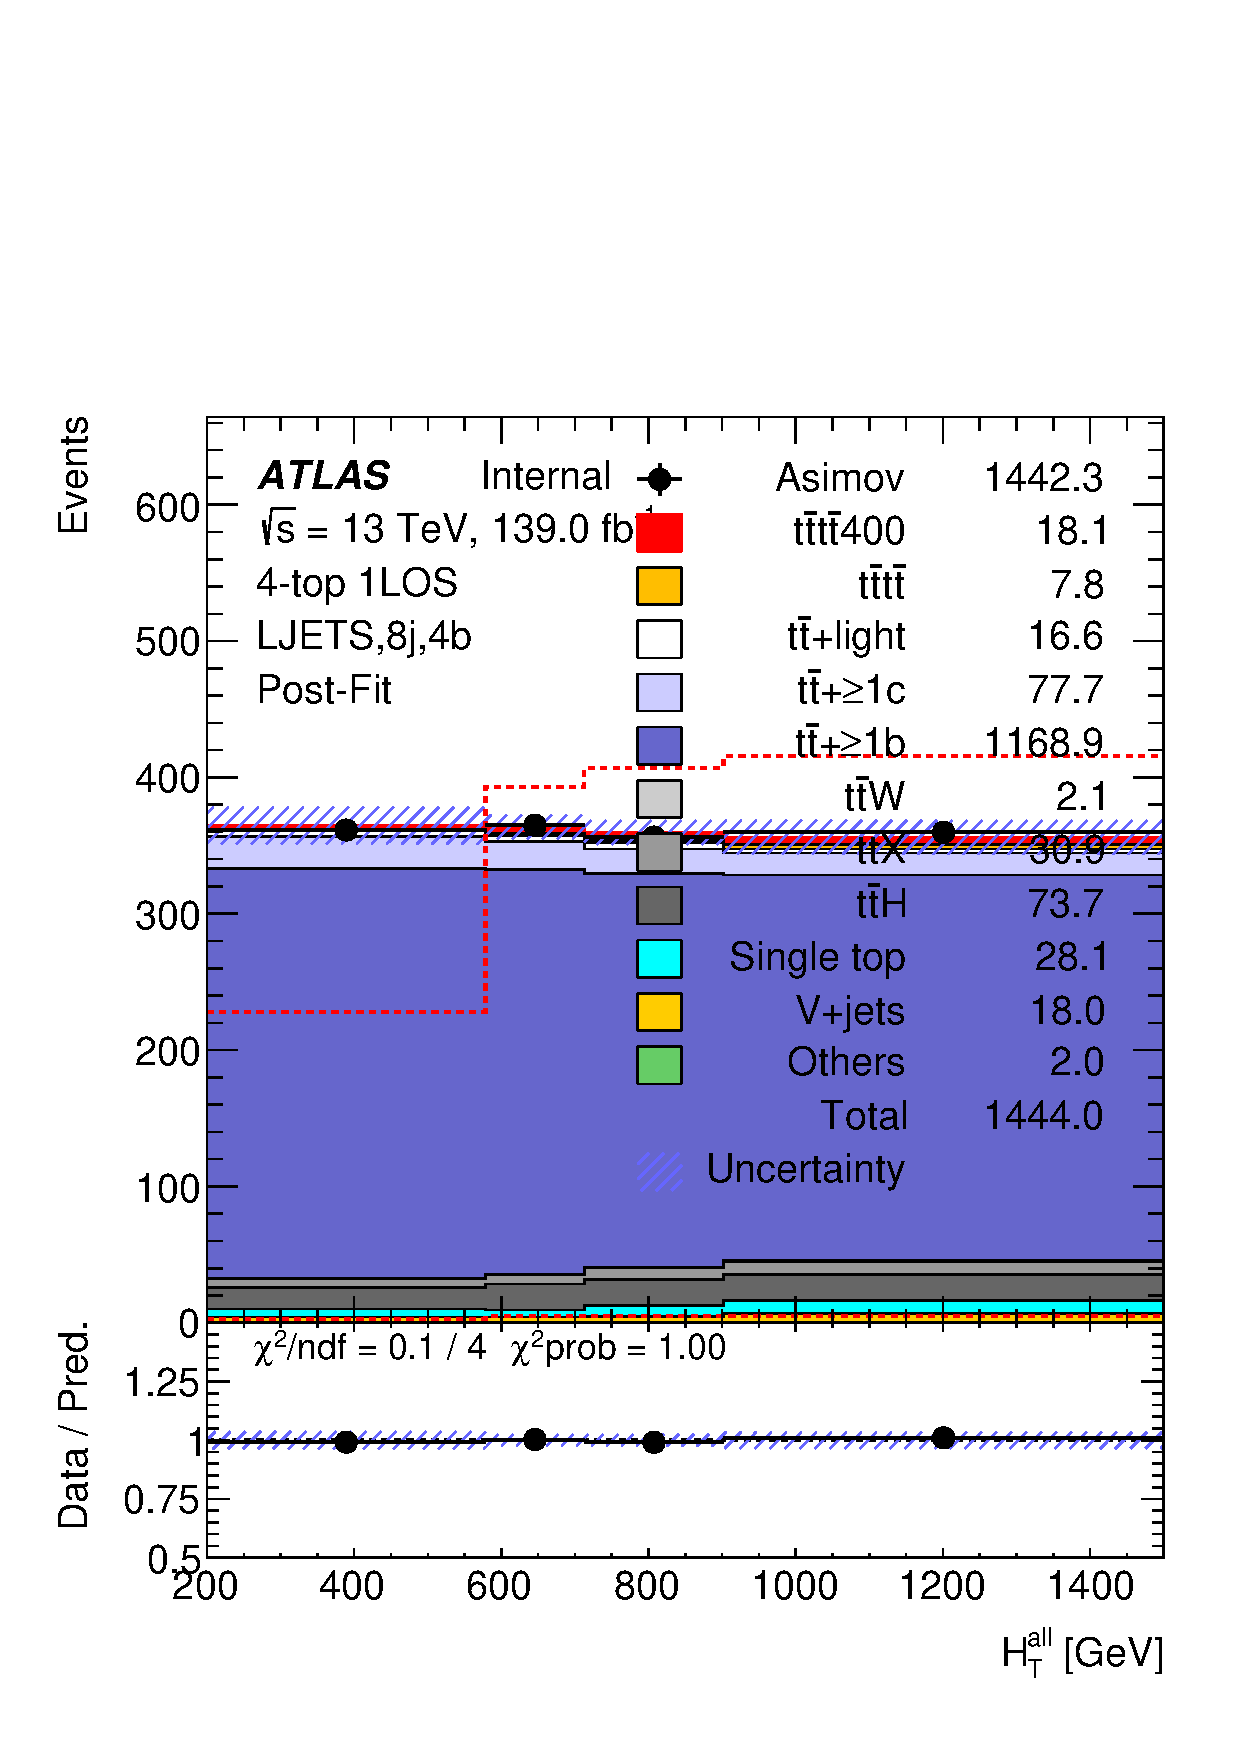
\includegraphics[width=0.23 \textwidth]{figures/4FS_studies/dataMC_4FSsyst_norew/ljets_8j4b_postFit.pdf} &
        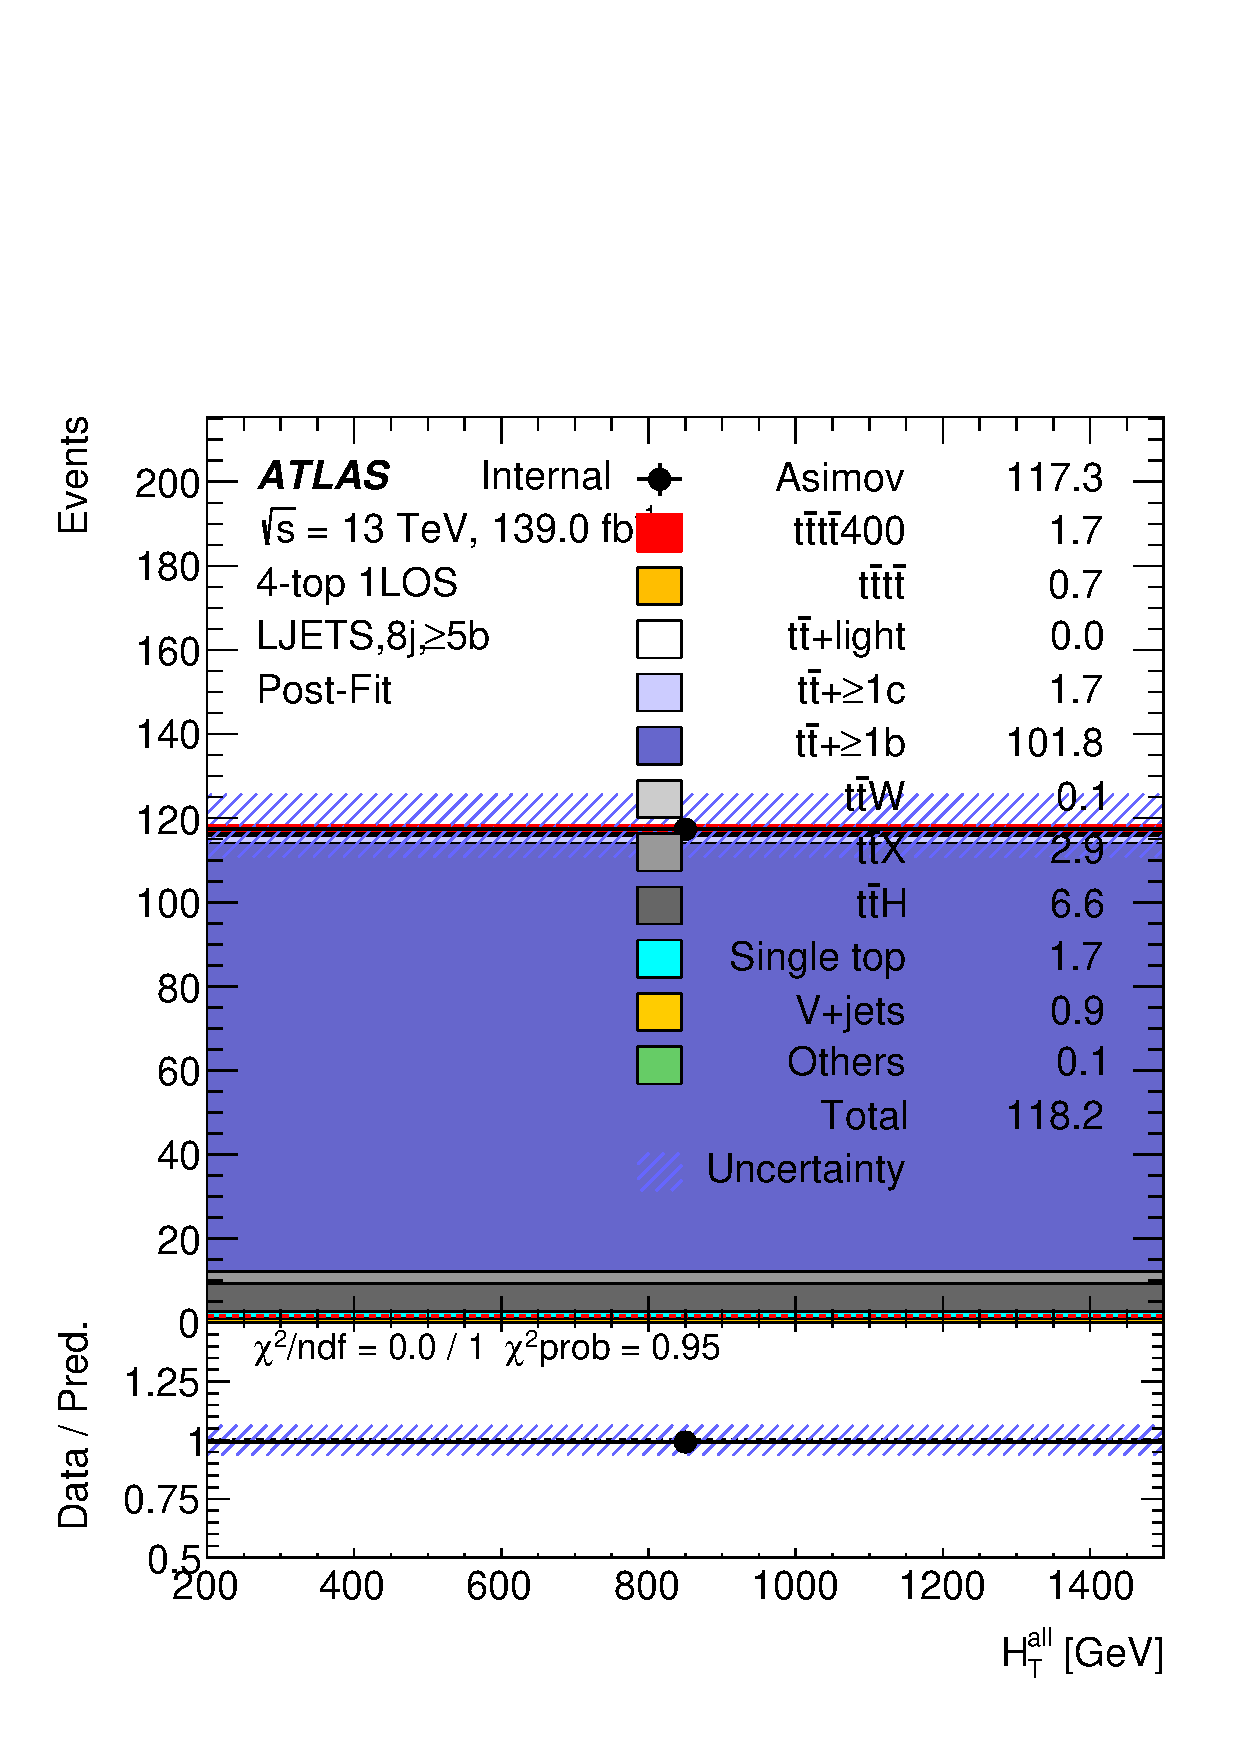
\includegraphics[width=0.23 \textwidth]{figures/4FS_studies/dataMC_4FSsyst_norew/ljets_8jge5b_postFit.pdf}\\

        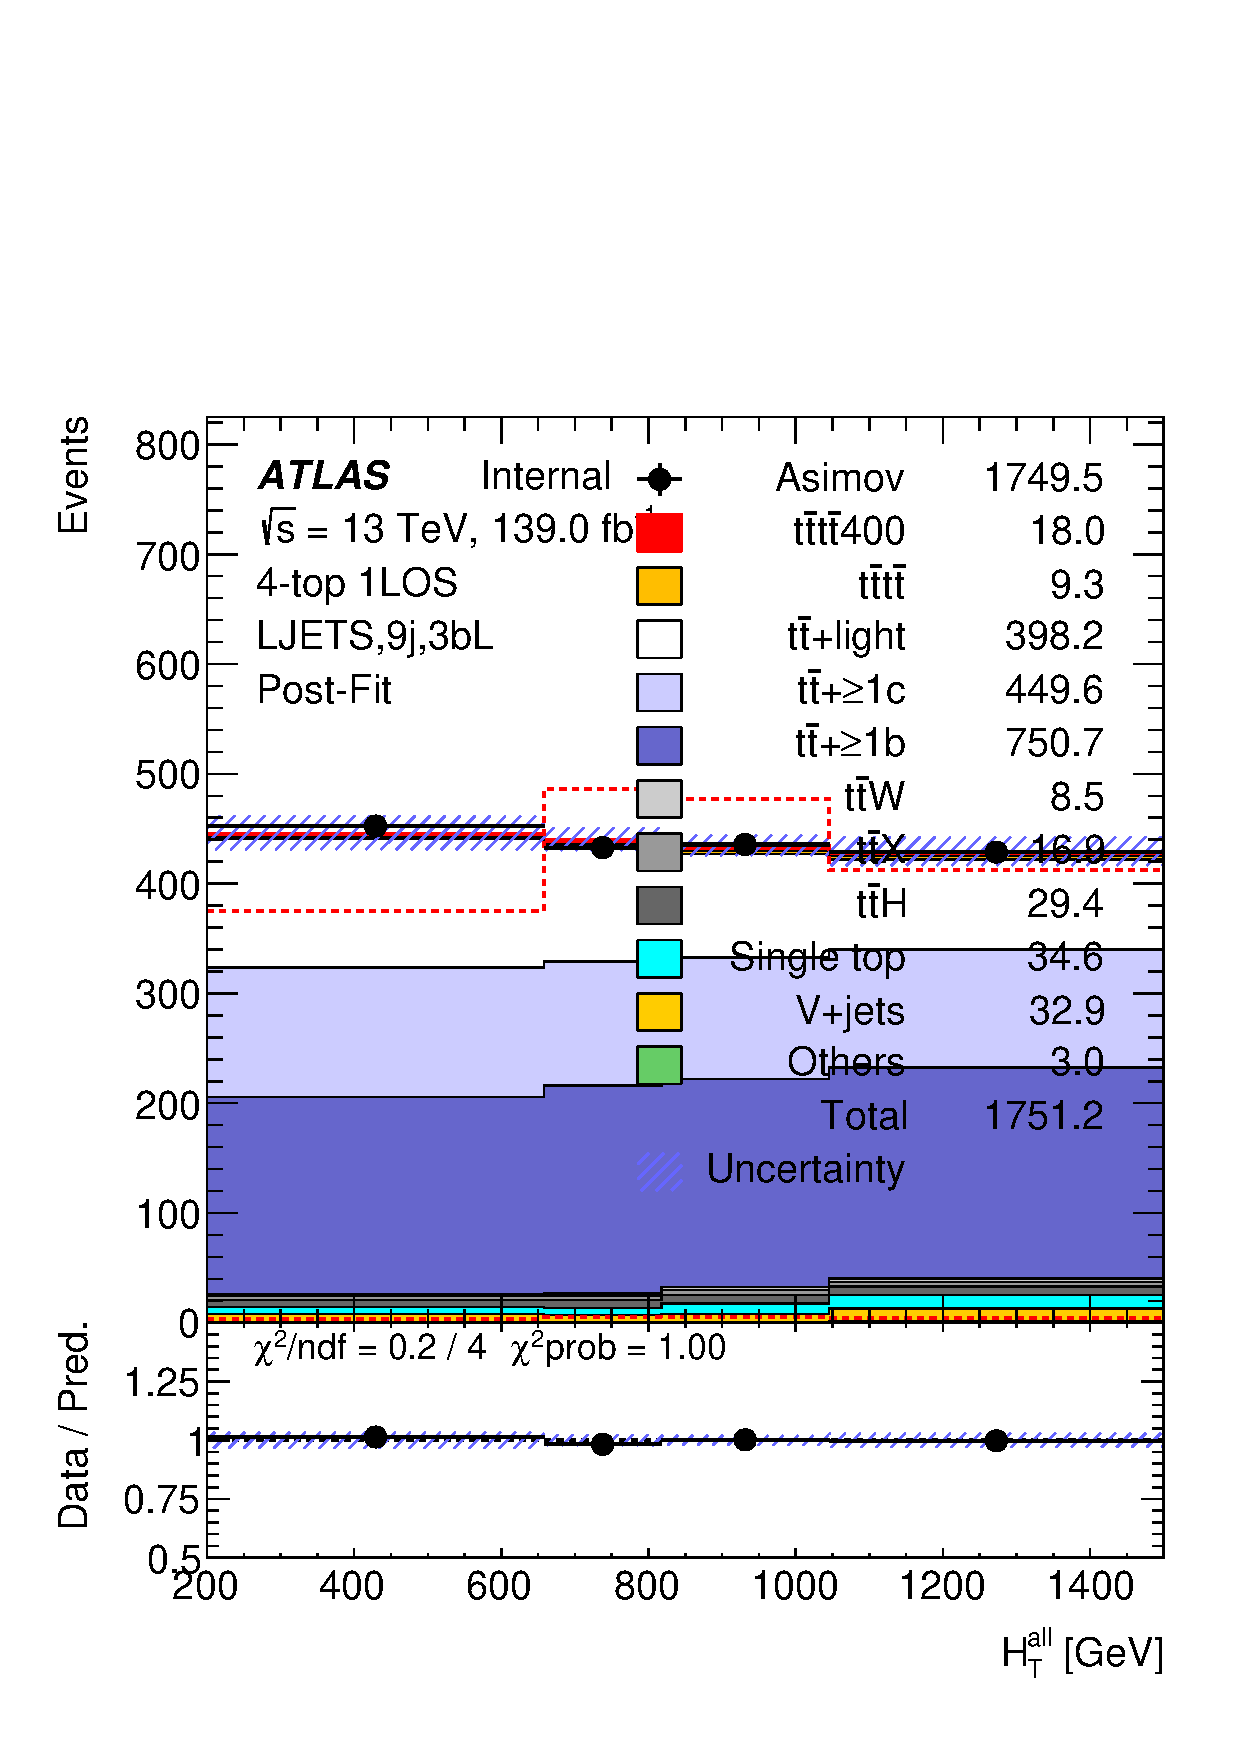
\includegraphics[width=0.23 \textwidth]{figures/4FS_studies/dataMC_4FSsyst_norew/ljets_9j3bL_postFit.pdf} &
        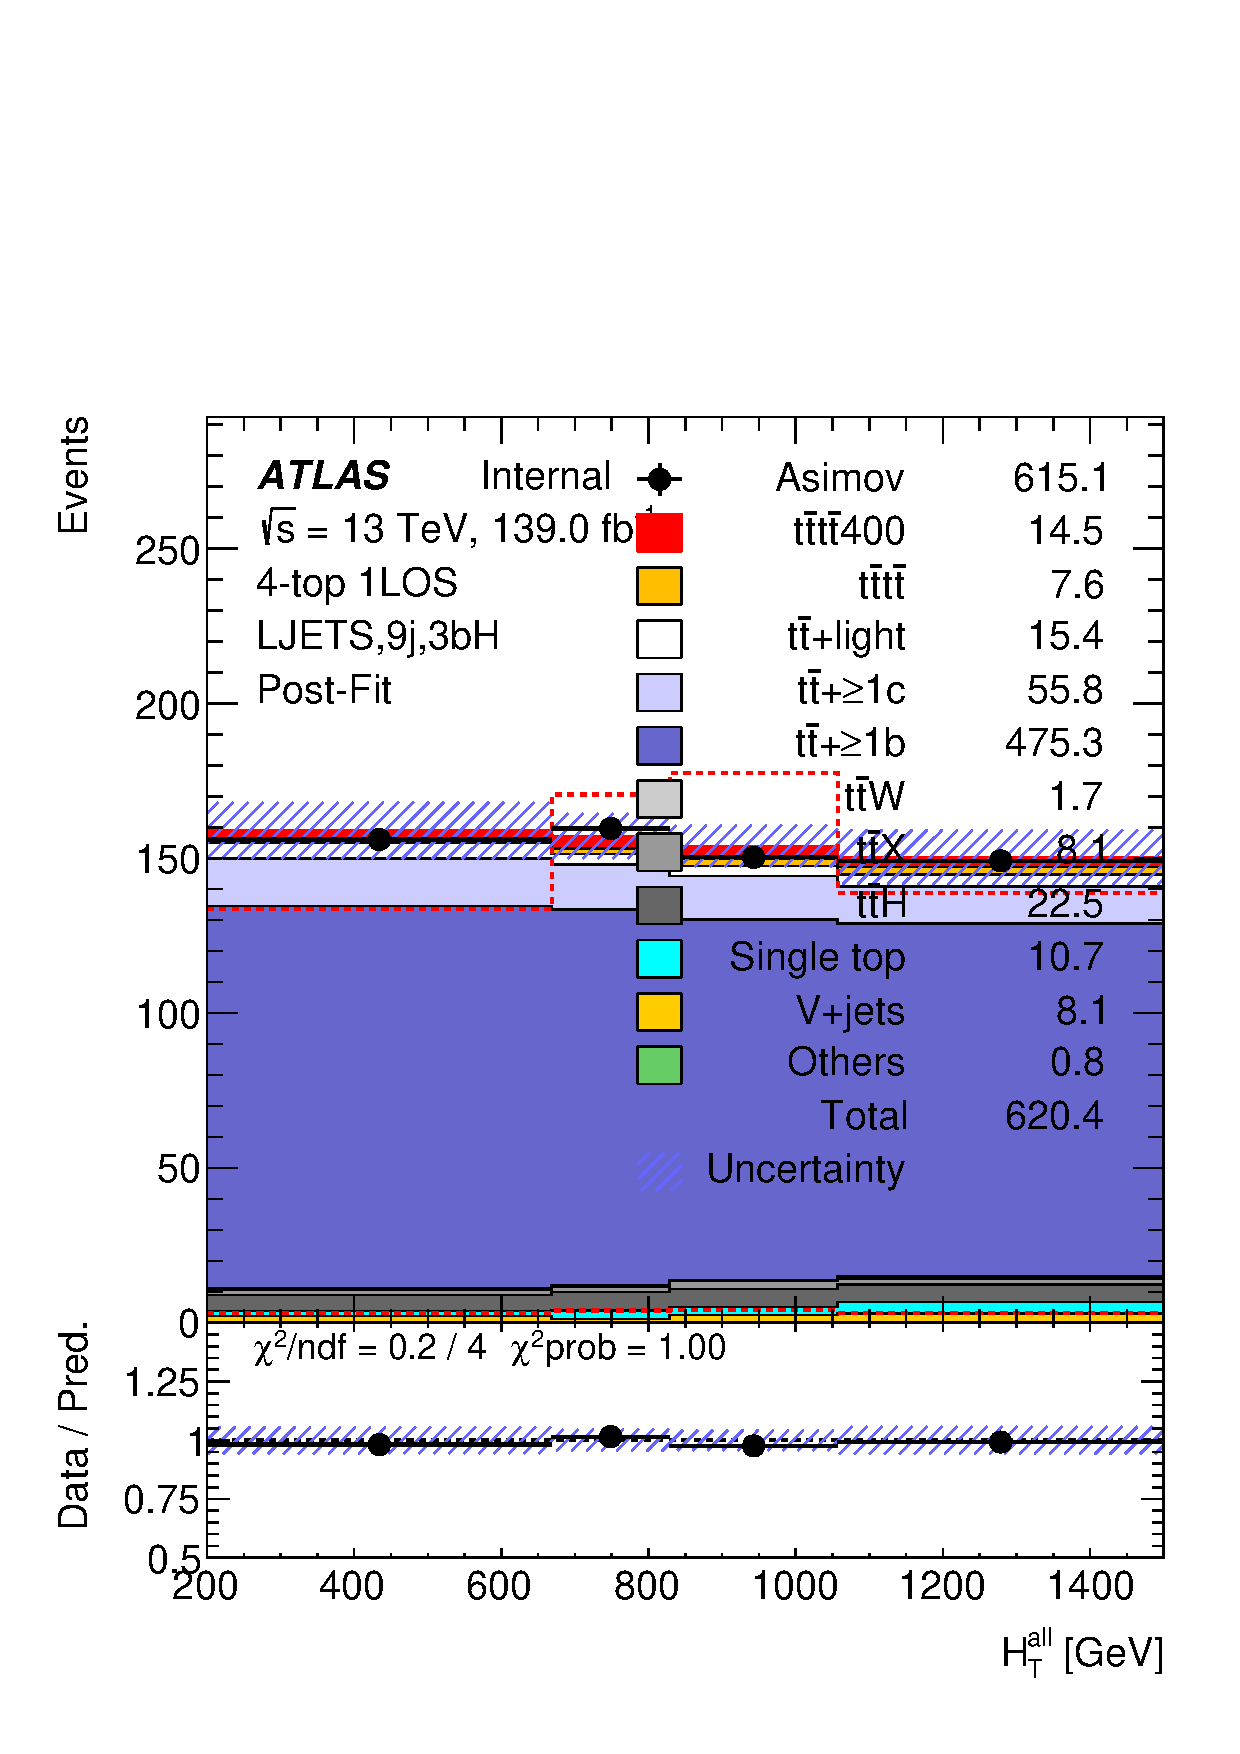
\includegraphics[width=0.23 \textwidth]{figures/4FS_studies/dataMC_4FSsyst_norew/ljets_9j3bH_postFit.pdf} &
        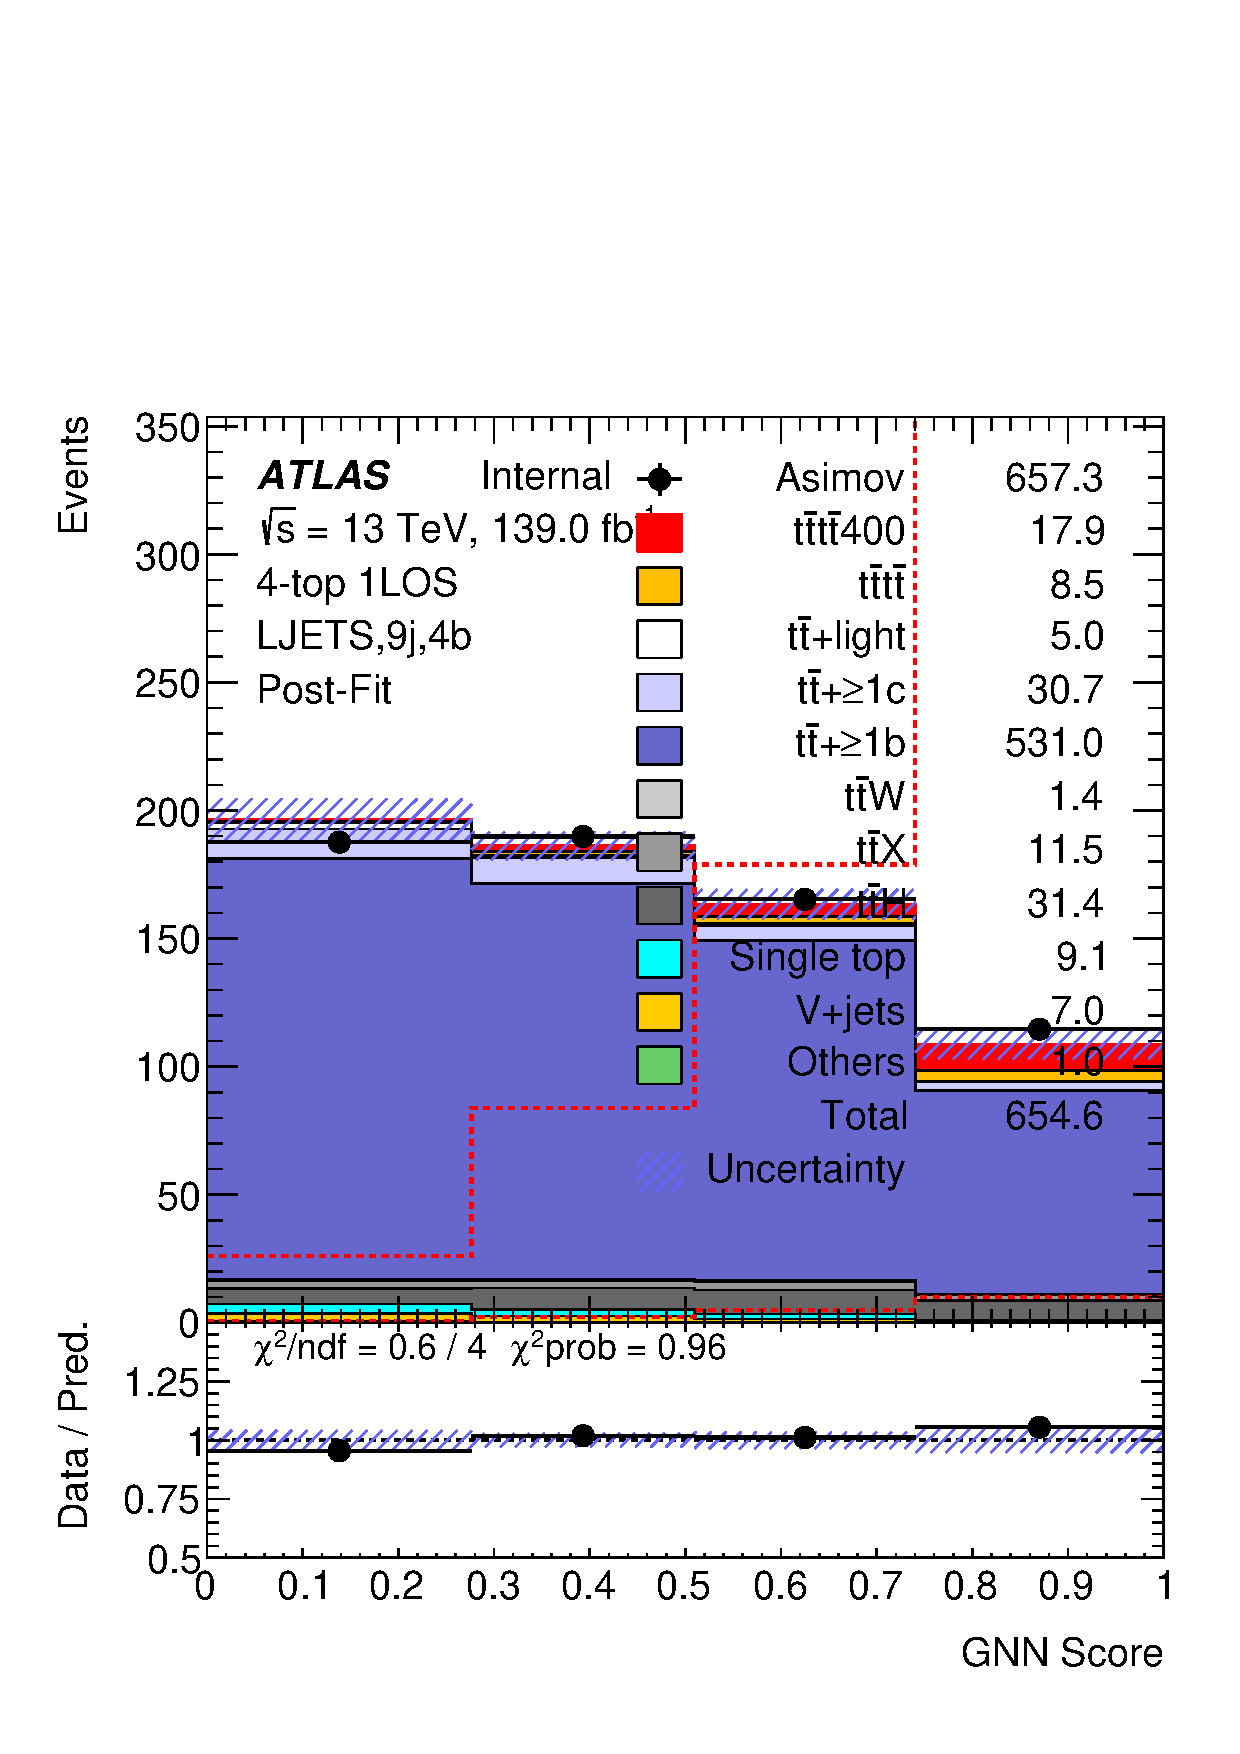
\includegraphics[width=0.23 \textwidth]{figures/4FS_studies/dataMC_4FSsyst_norew/ljets_9j4b_postFit.pdf} &
        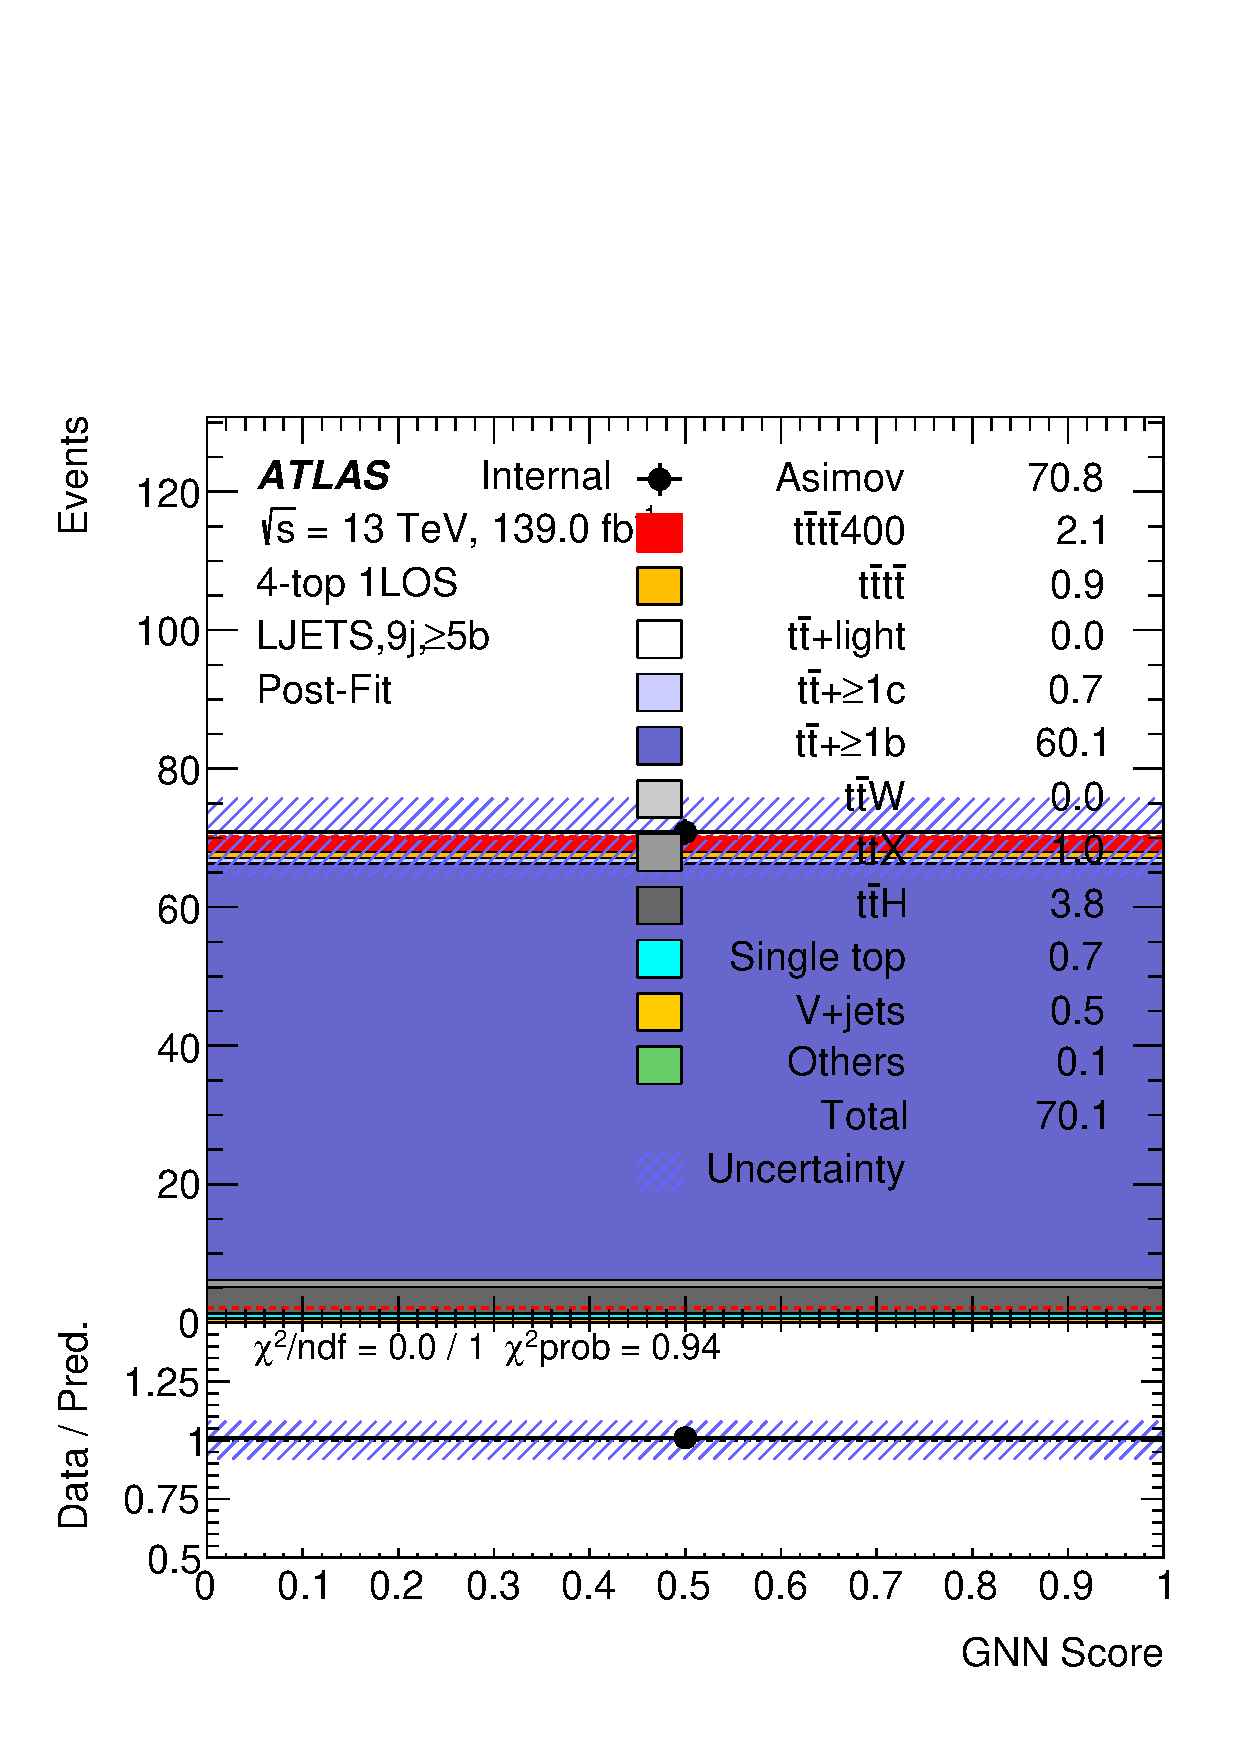
\includegraphics[width=0.23 \textwidth]{figures/4FS_studies/dataMC_4FSsyst_norew/ljets_9jge5b_postFit.pdf} \\

        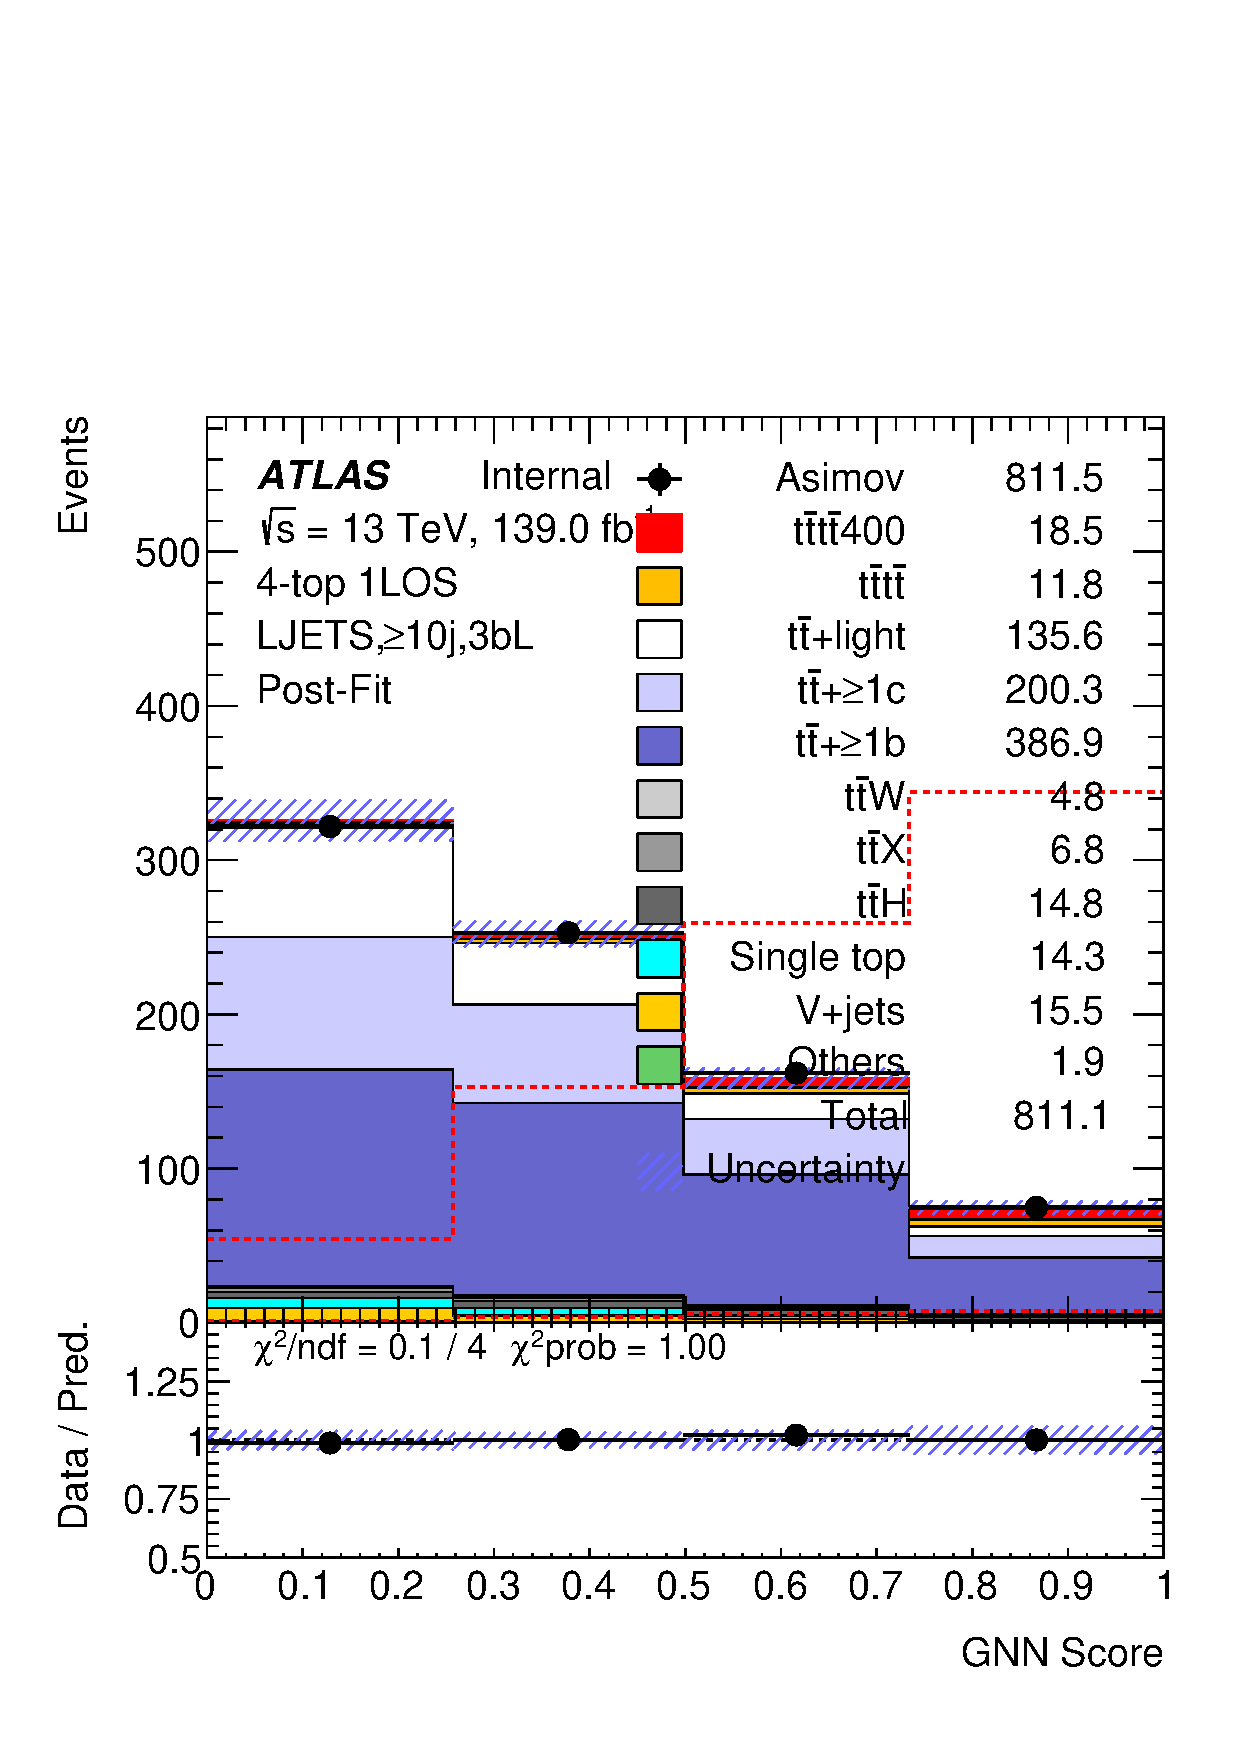
\includegraphics[width=0.23 \textwidth]{figures/4FS_studies/dataMC_4FSsyst_norew/ljets_ge10j3bL_postFit.pdf} &
        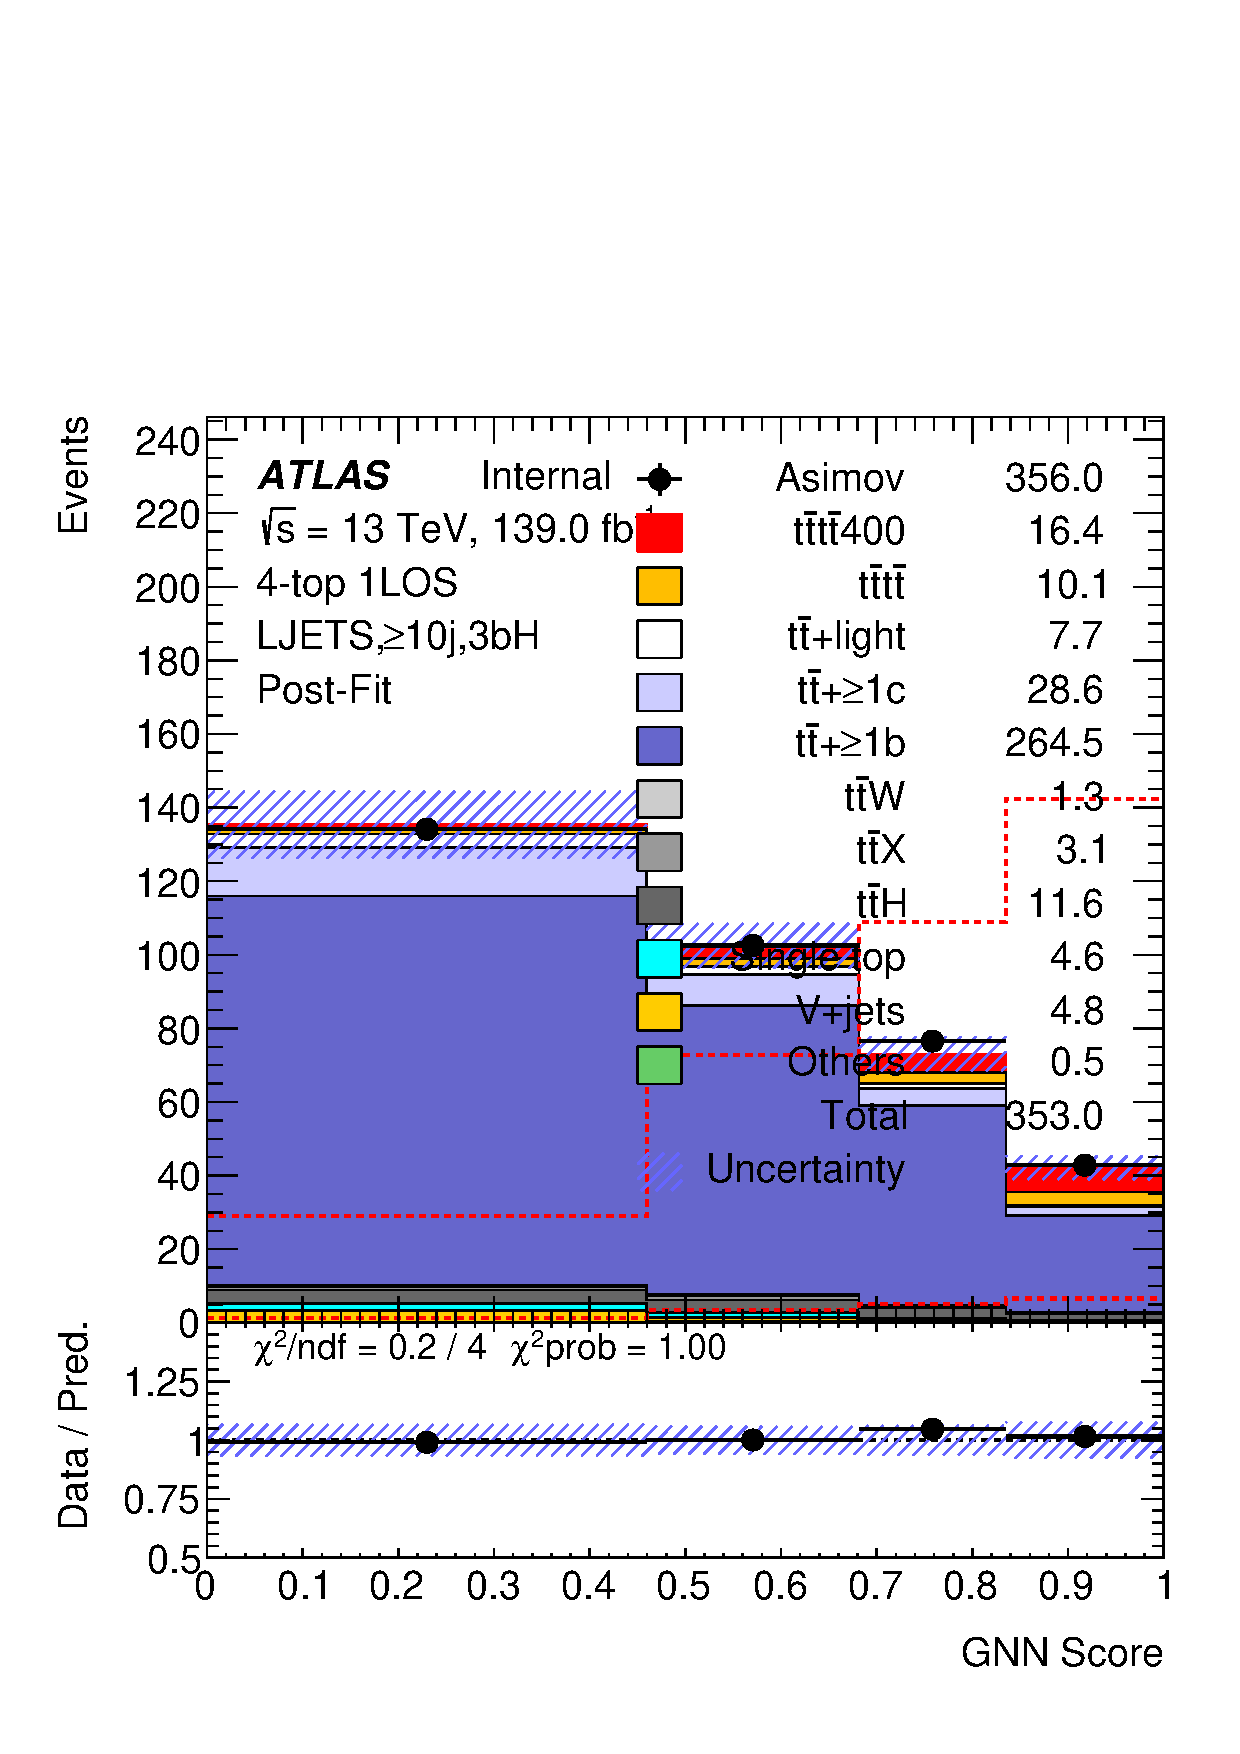
\includegraphics[width=0.23 \textwidth]{figures/4FS_studies/dataMC_4FSsyst_norew/ljets_ge10j3bH_postFit.pdf} &
        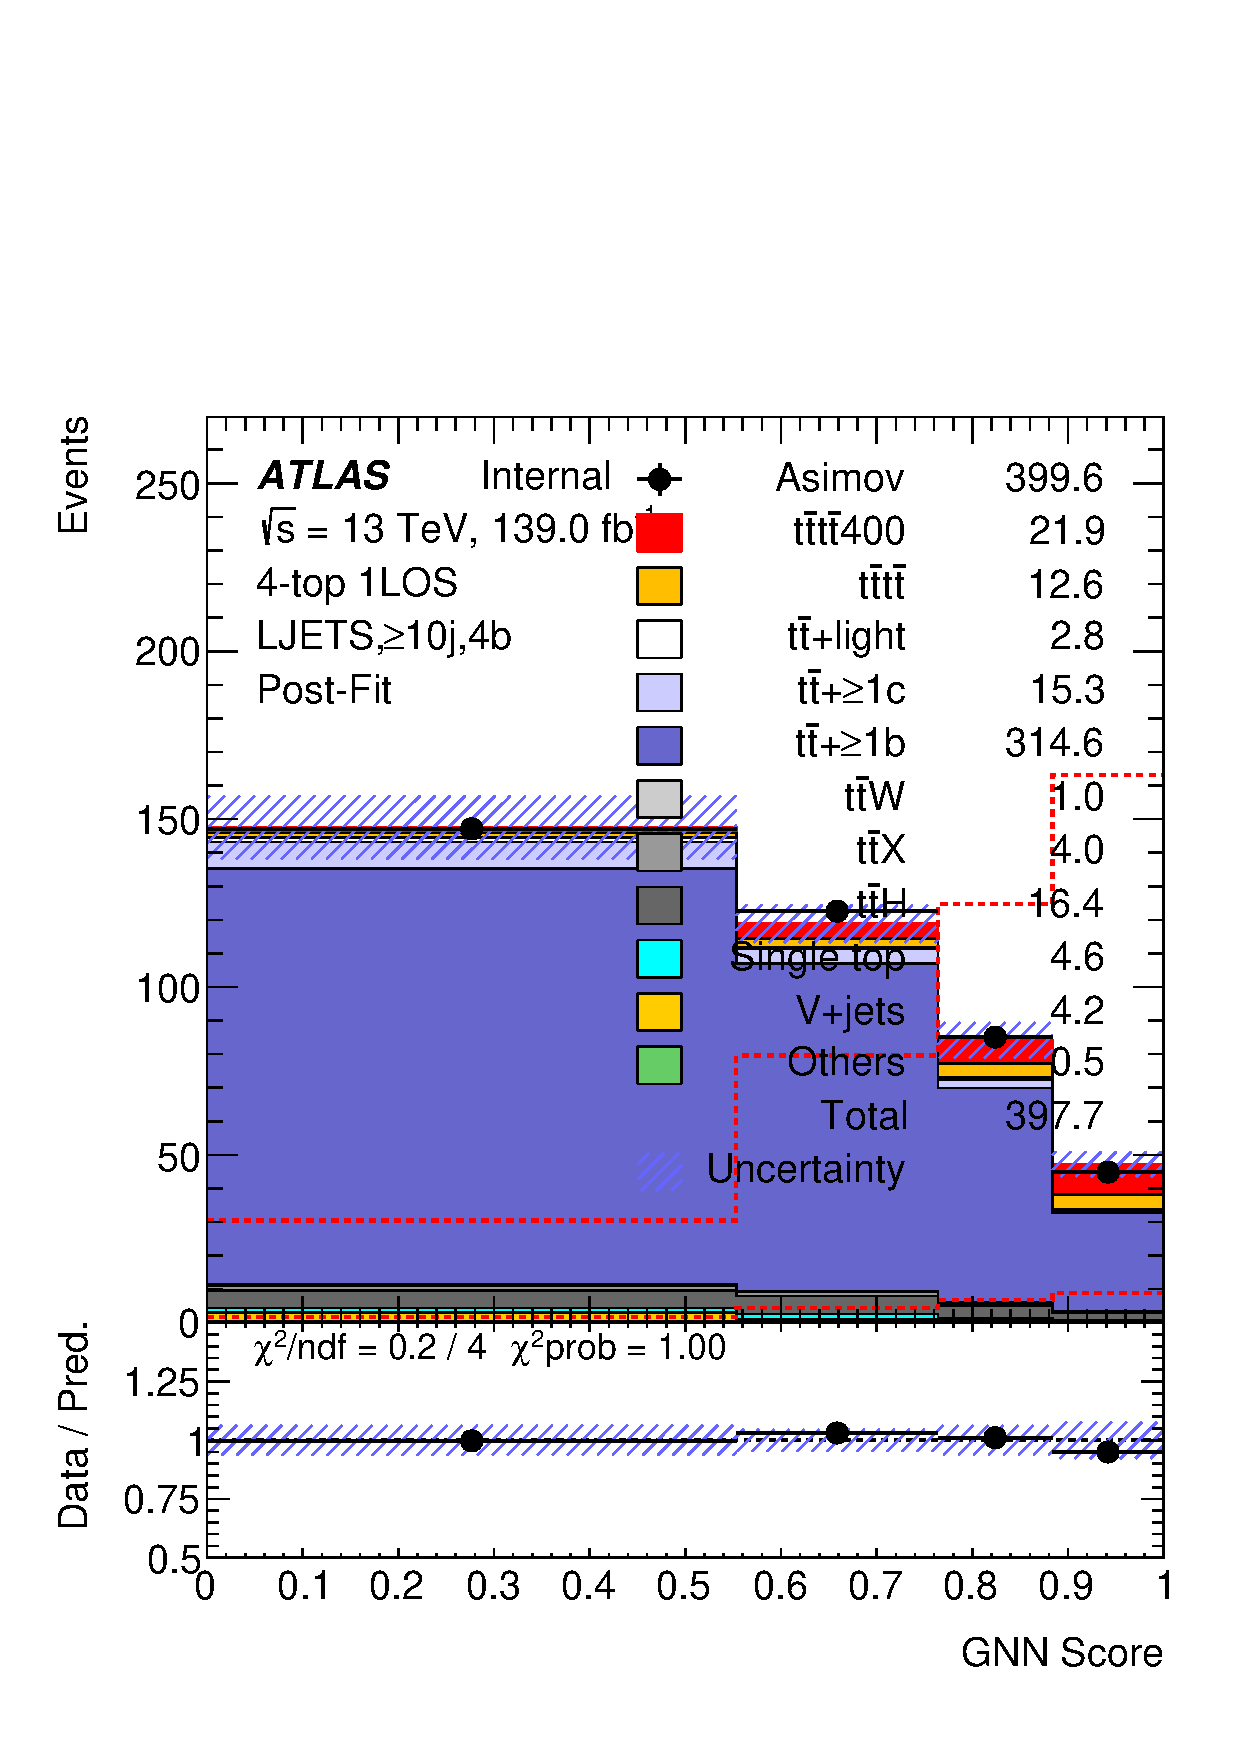
\includegraphics[width=0.23 \textwidth]{figures/4FS_studies/dataMC_4FSsyst_norew/ljets_ge10j4b_postFit.pdf} &
        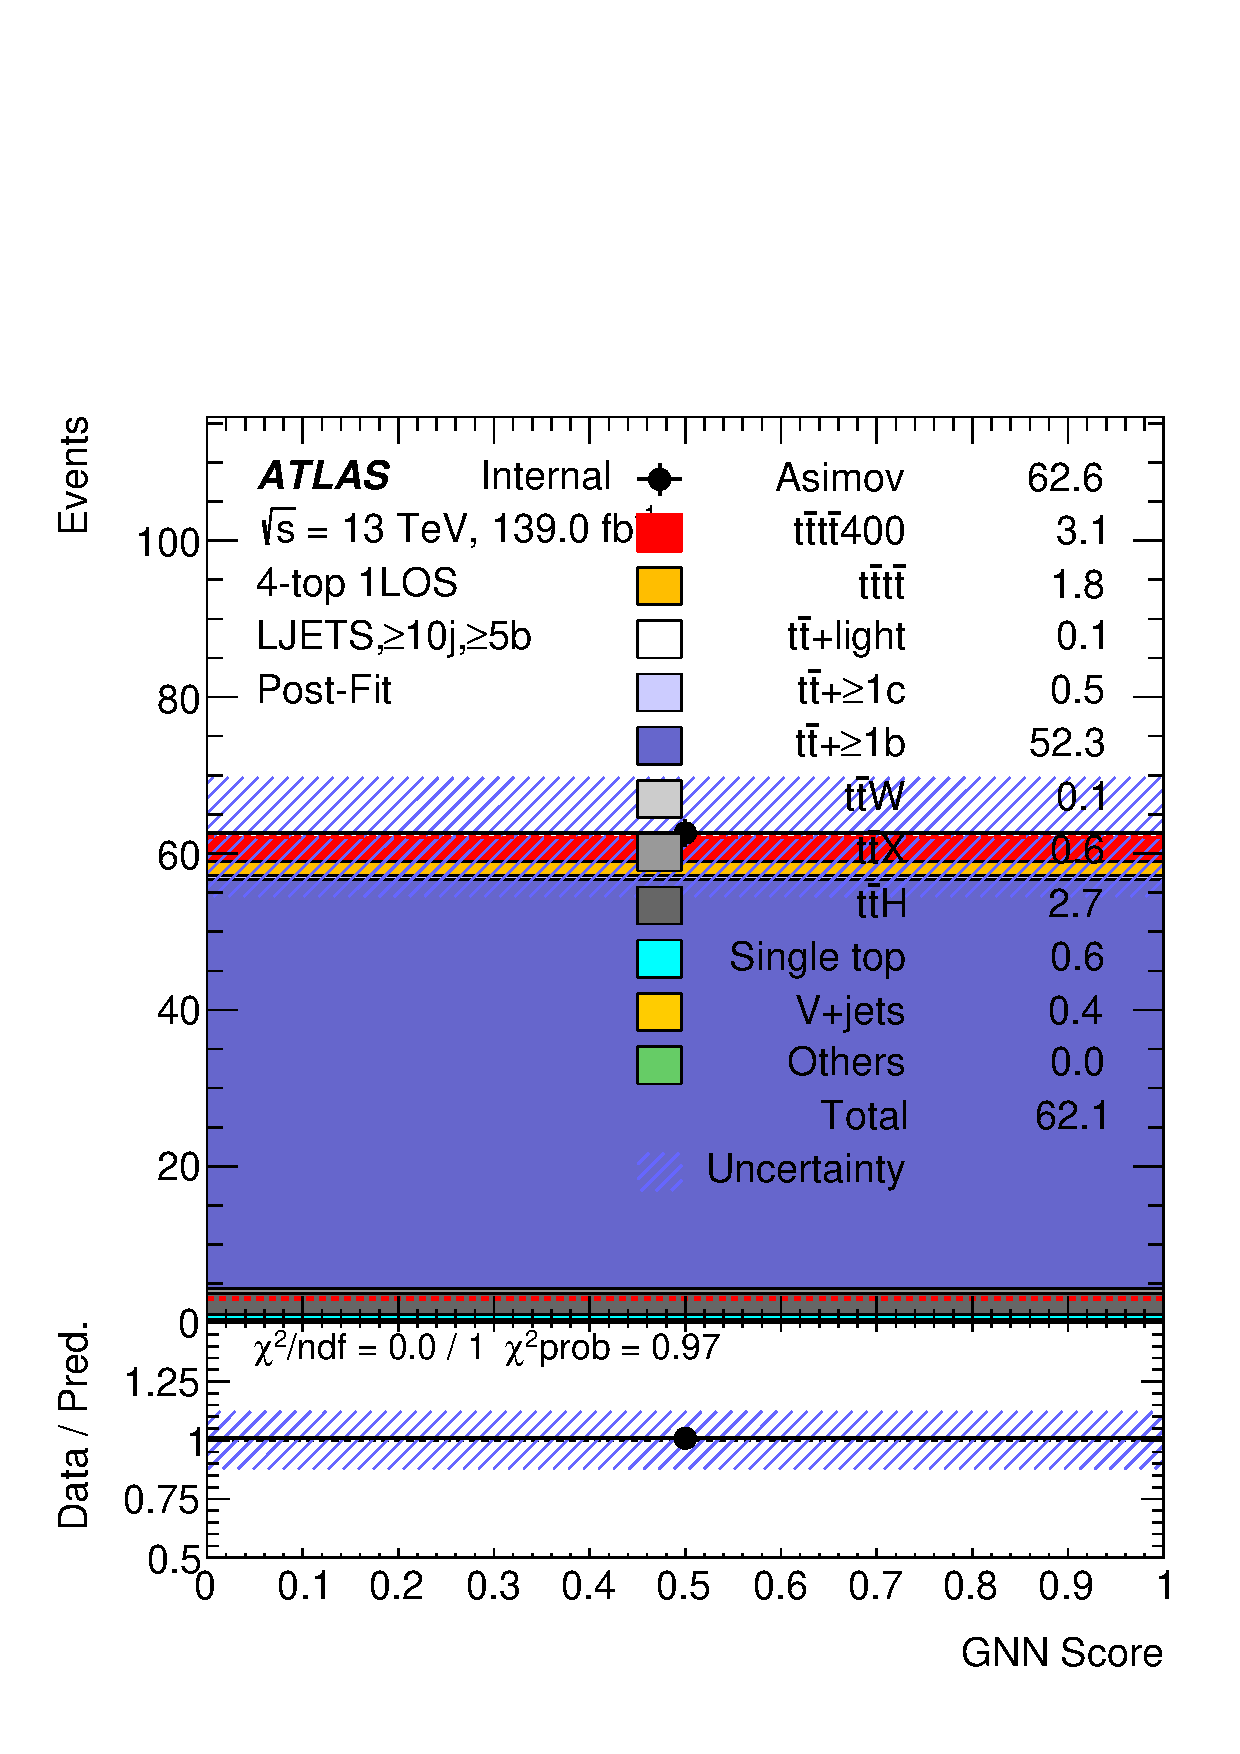
\includegraphics[width=0.23 \textwidth]{figures/4FS_studies/dataMC_4FSsyst_norew/ljets_ge10jge5b_postFit.pdf} \\
        \end{tabular}
        \caption{\label{fig:4FS_dataMC_4FSsyst_norew_1L_postfit}Post-fit comparison of the 1L regions between samples with $t\bar{t}$ TTB samples produced with 5FS (MC) and $t\bar{t}$ TTB samples produced with 4FS (set as `pseudodata'). All systematics including 4FS systematics are incorporated in the uncertainty. The $t\bar{t}$ samples are not reweighted.}
\end{center}
\end{figure}

\begin{figure}[htbp!]
        \begin{center} \setlength{\tabcolsep}{2.5pt}\footnotesize
        \begin{tabular}{ccc}
        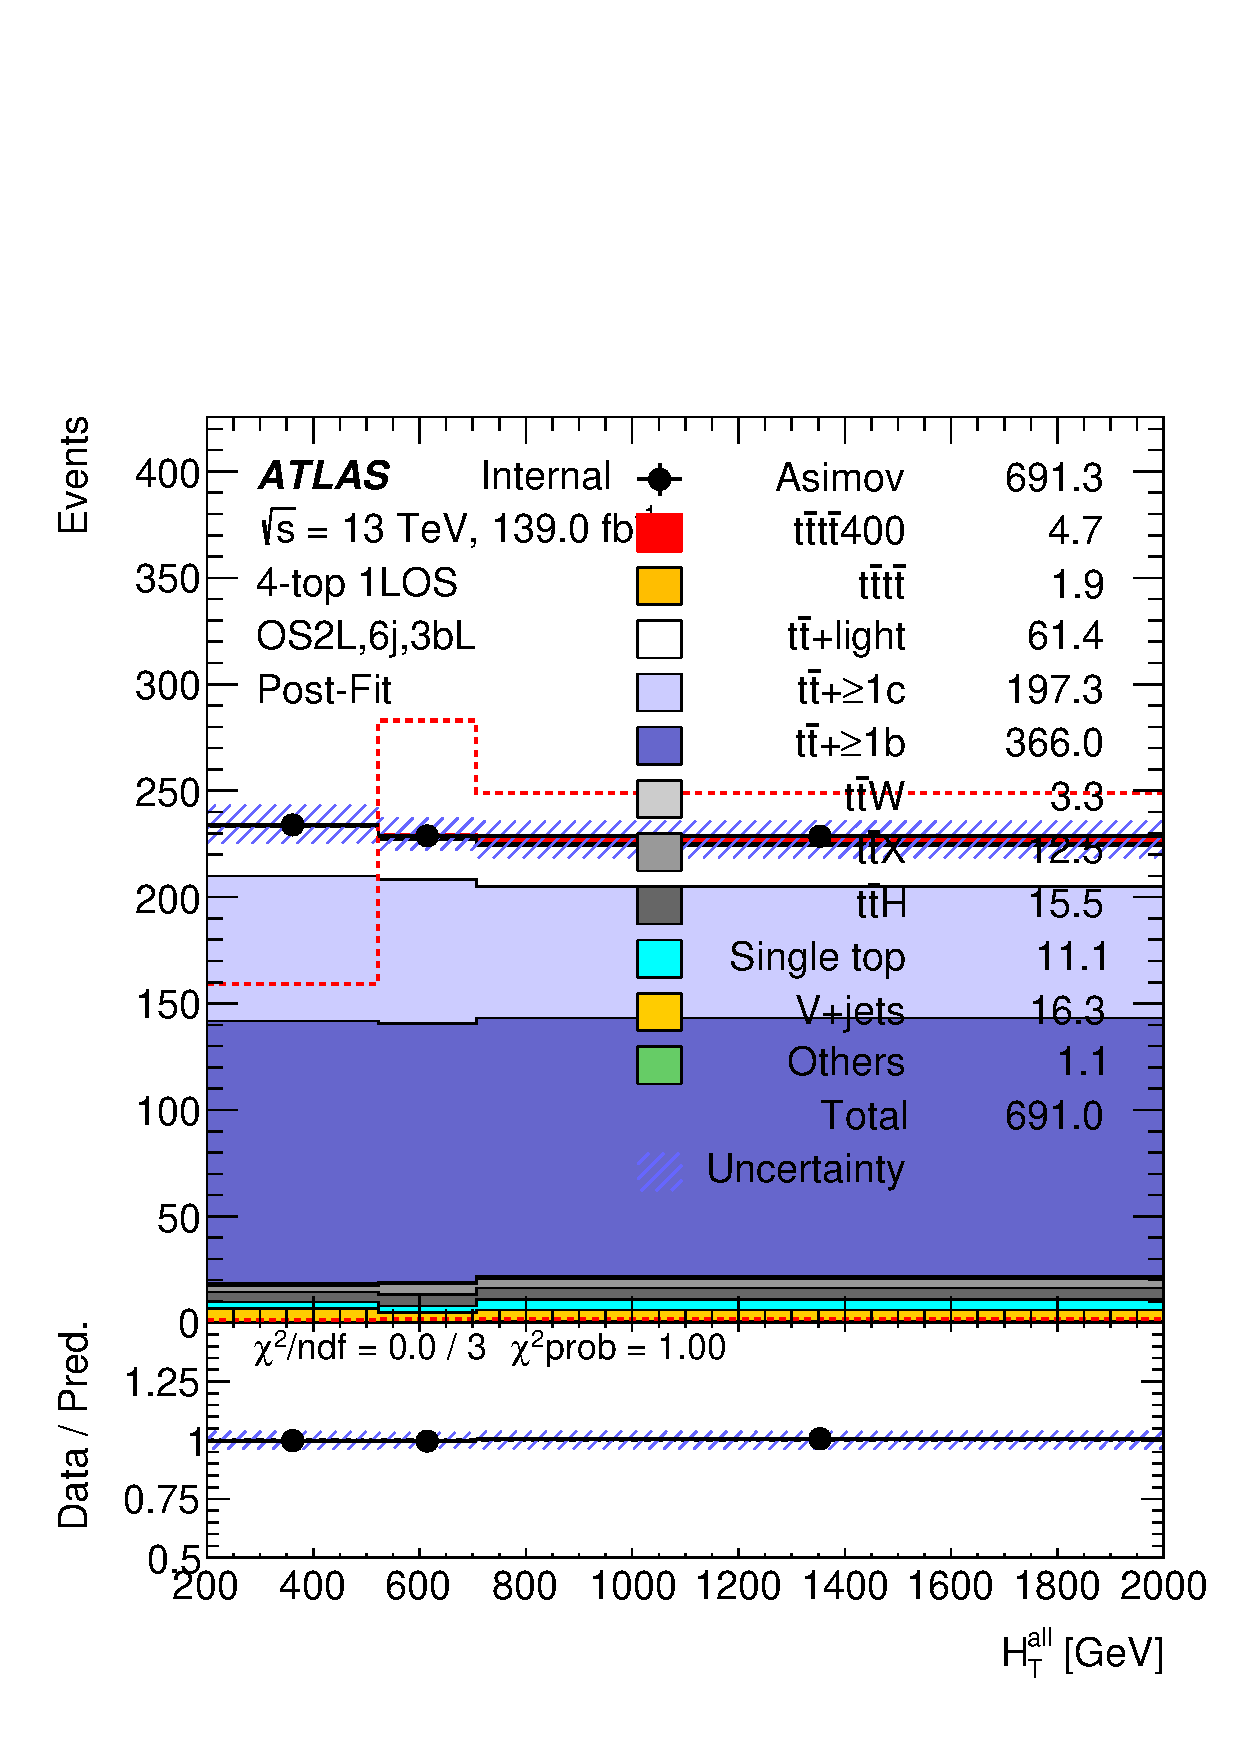
\includegraphics[width=0.31 \textwidth]{figures/4FS_studies/dataMC_4FSsyst_norew/os2l_6j3bL_postFit.pdf} &
        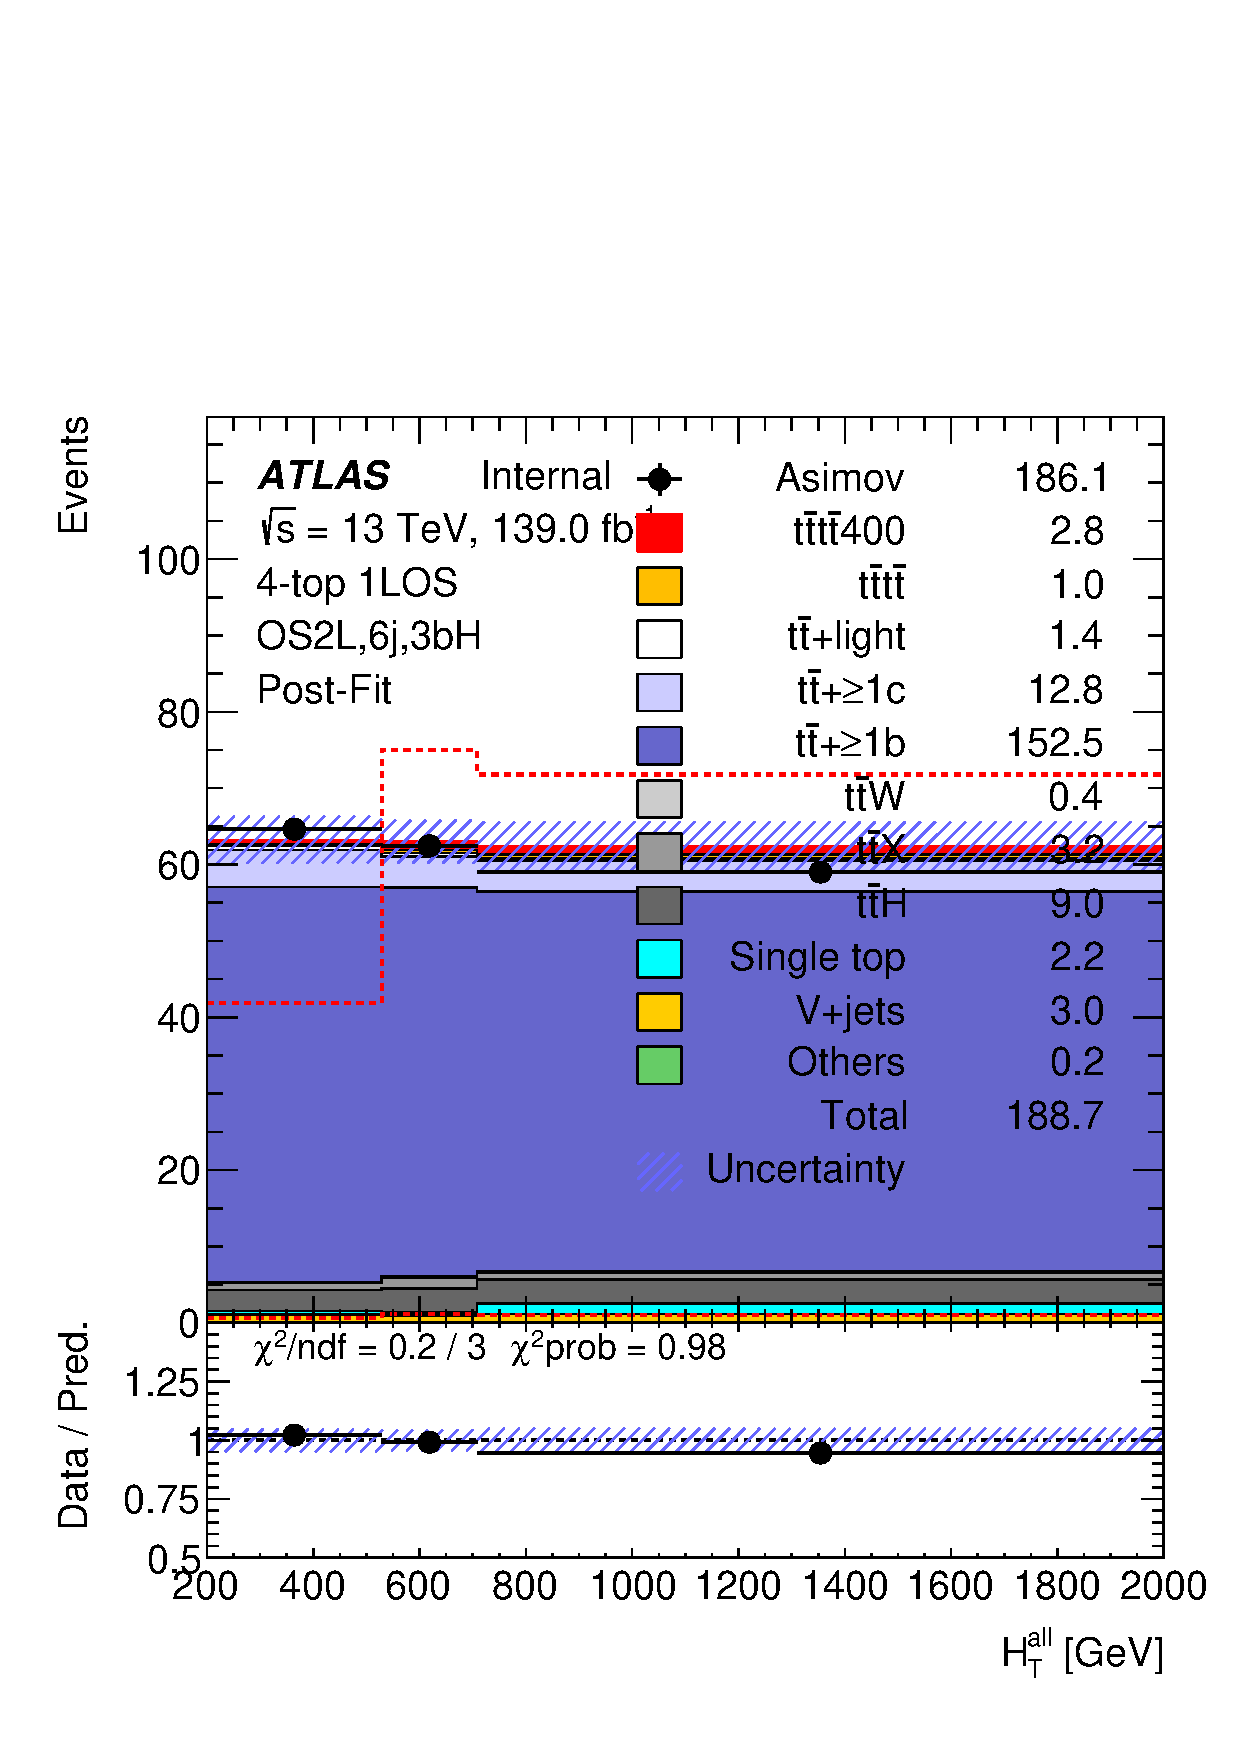
\includegraphics[width=0.31 \textwidth]{figures/4FS_studies/dataMC_4FSsyst_norew/os2l_6j3bH_postFit.pdf} &
        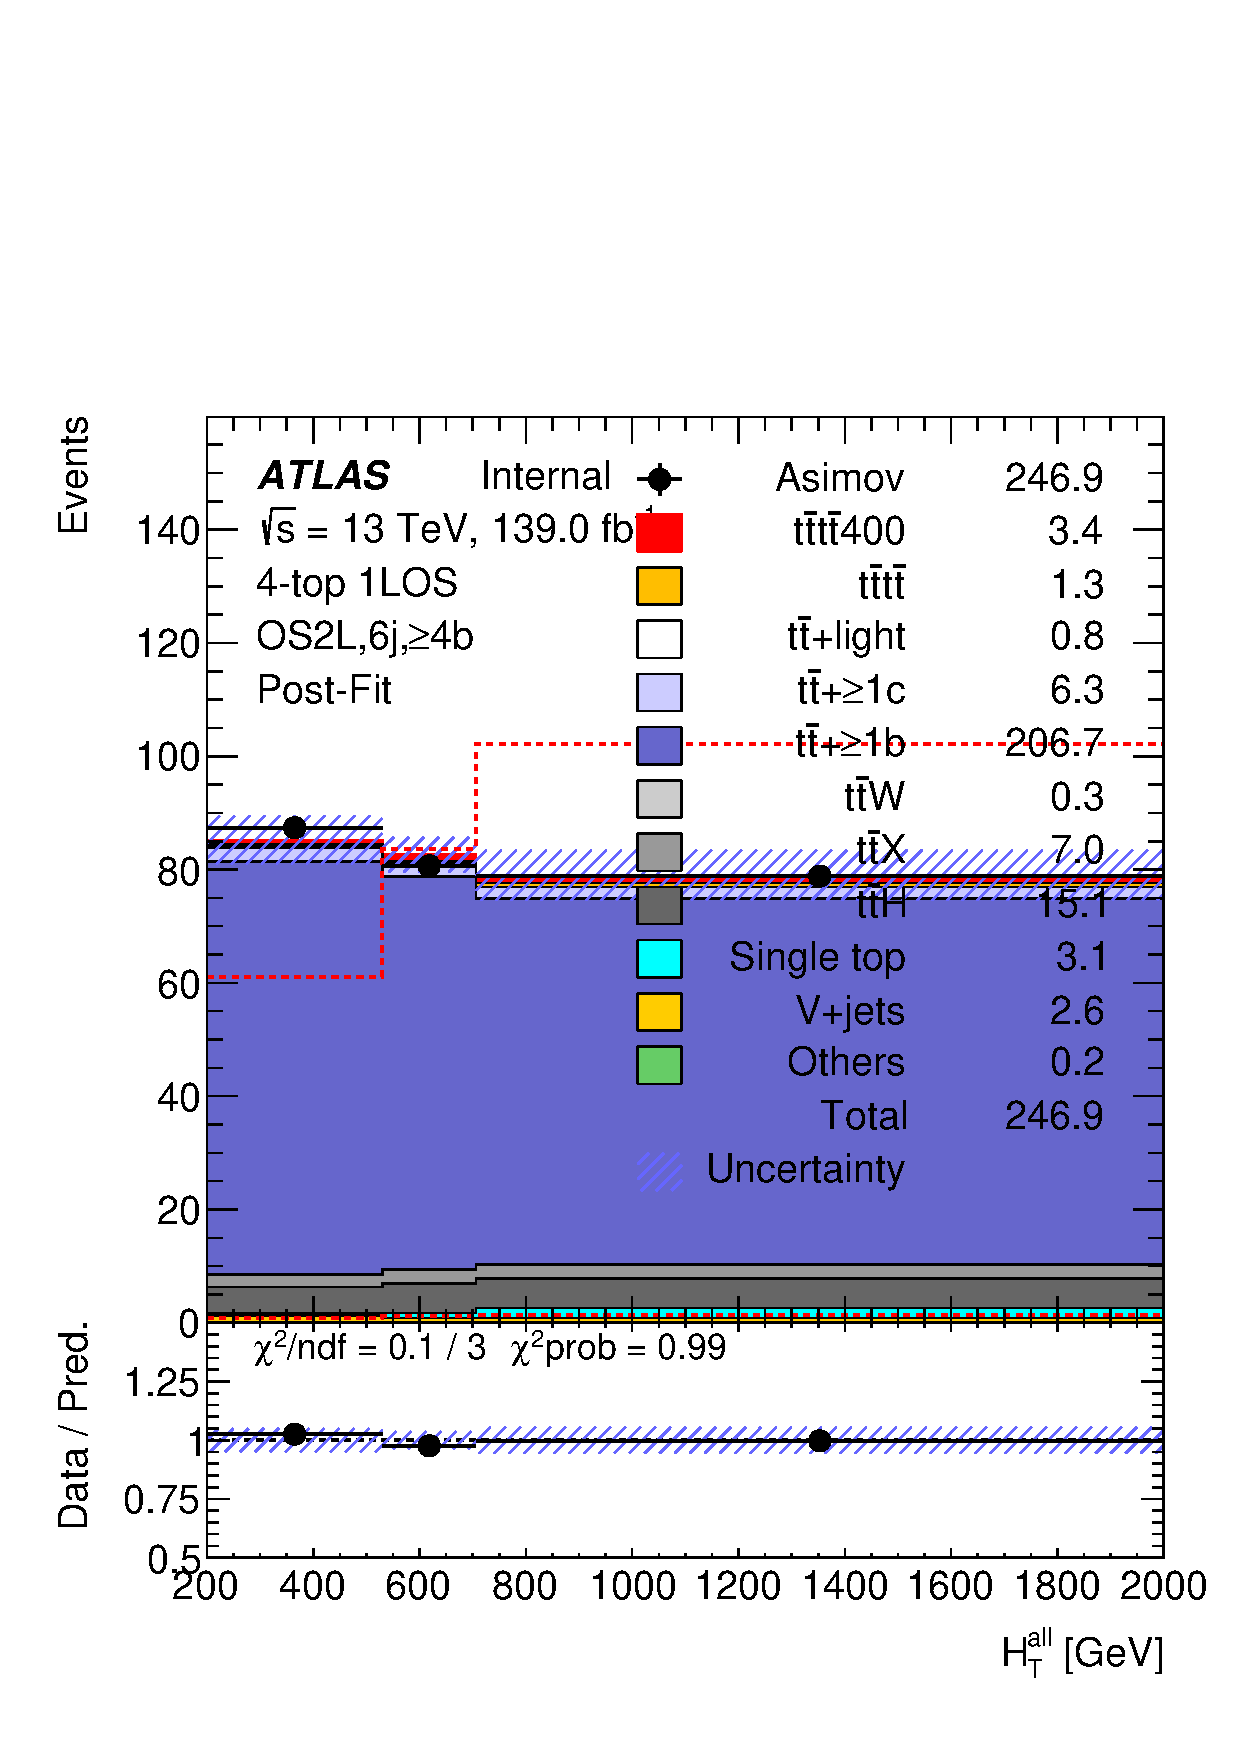
\includegraphics[width=0.31 \textwidth]{figures/4FS_studies/dataMC_4FSsyst_norew/os2l_6jge4b_postFit.pdf} \\

        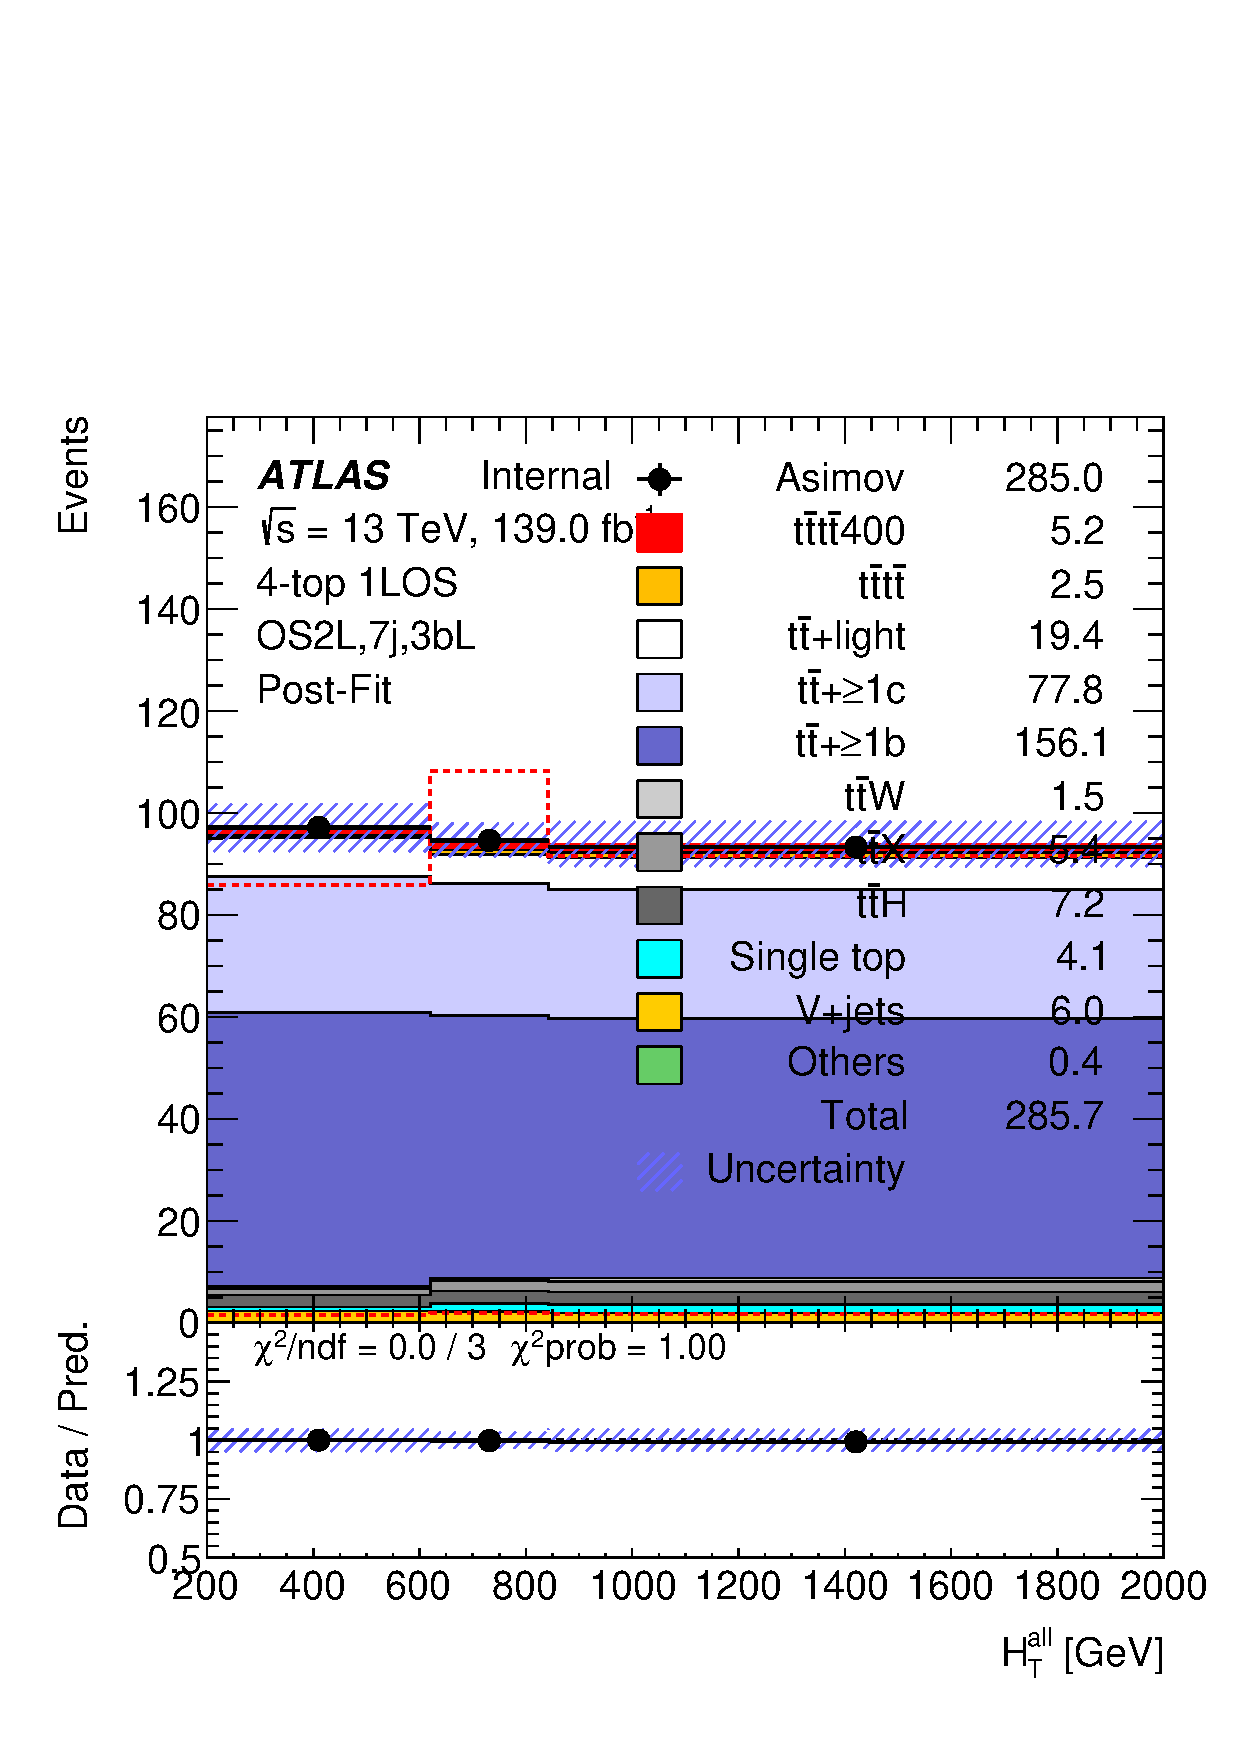
\includegraphics[width=0.31 \textwidth]{figures/4FS_studies/dataMC_4FSsyst_norew/os2l_7j3bL_postFit.pdf} &
        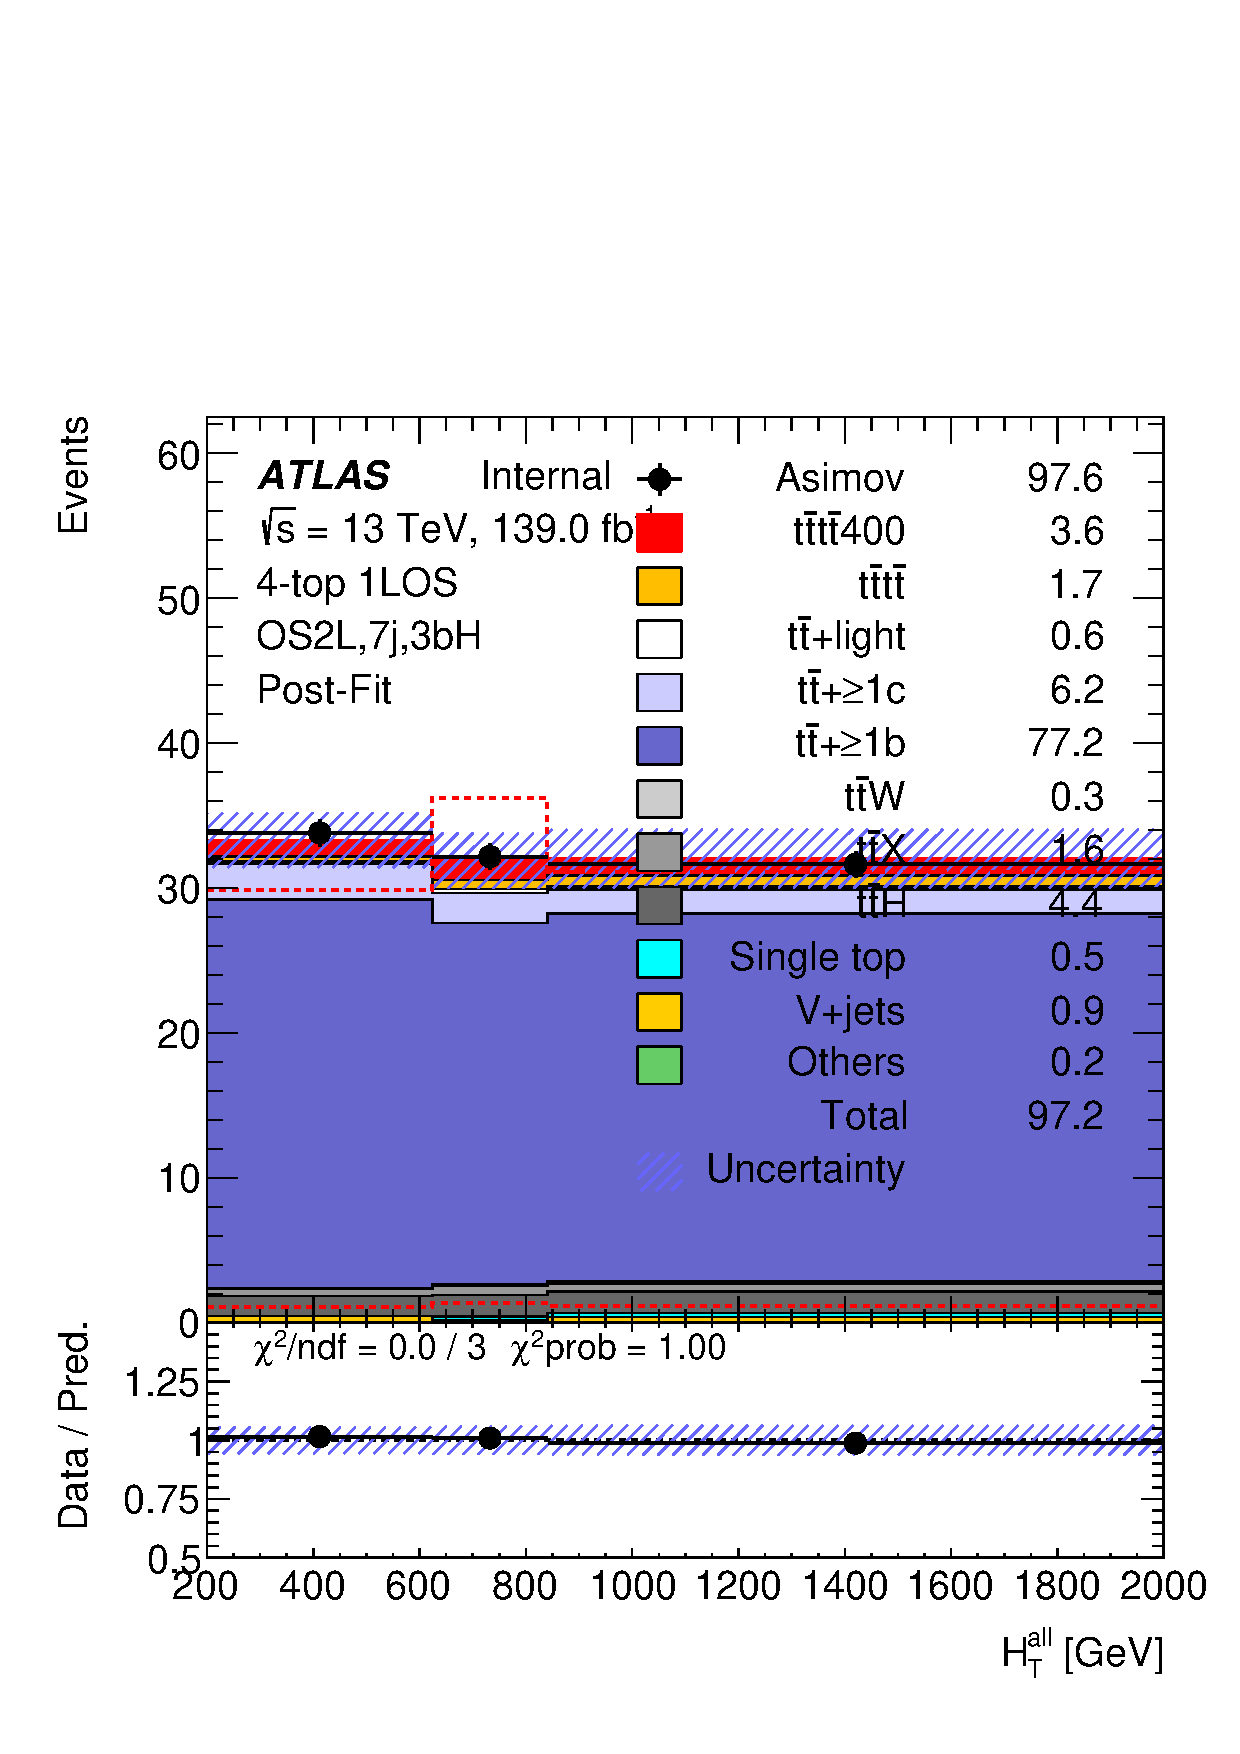
\includegraphics[width=0.31 \textwidth]{figures/4FS_studies/dataMC_4FSsyst_norew/os2l_7j3bH_postFit.pdf} &
        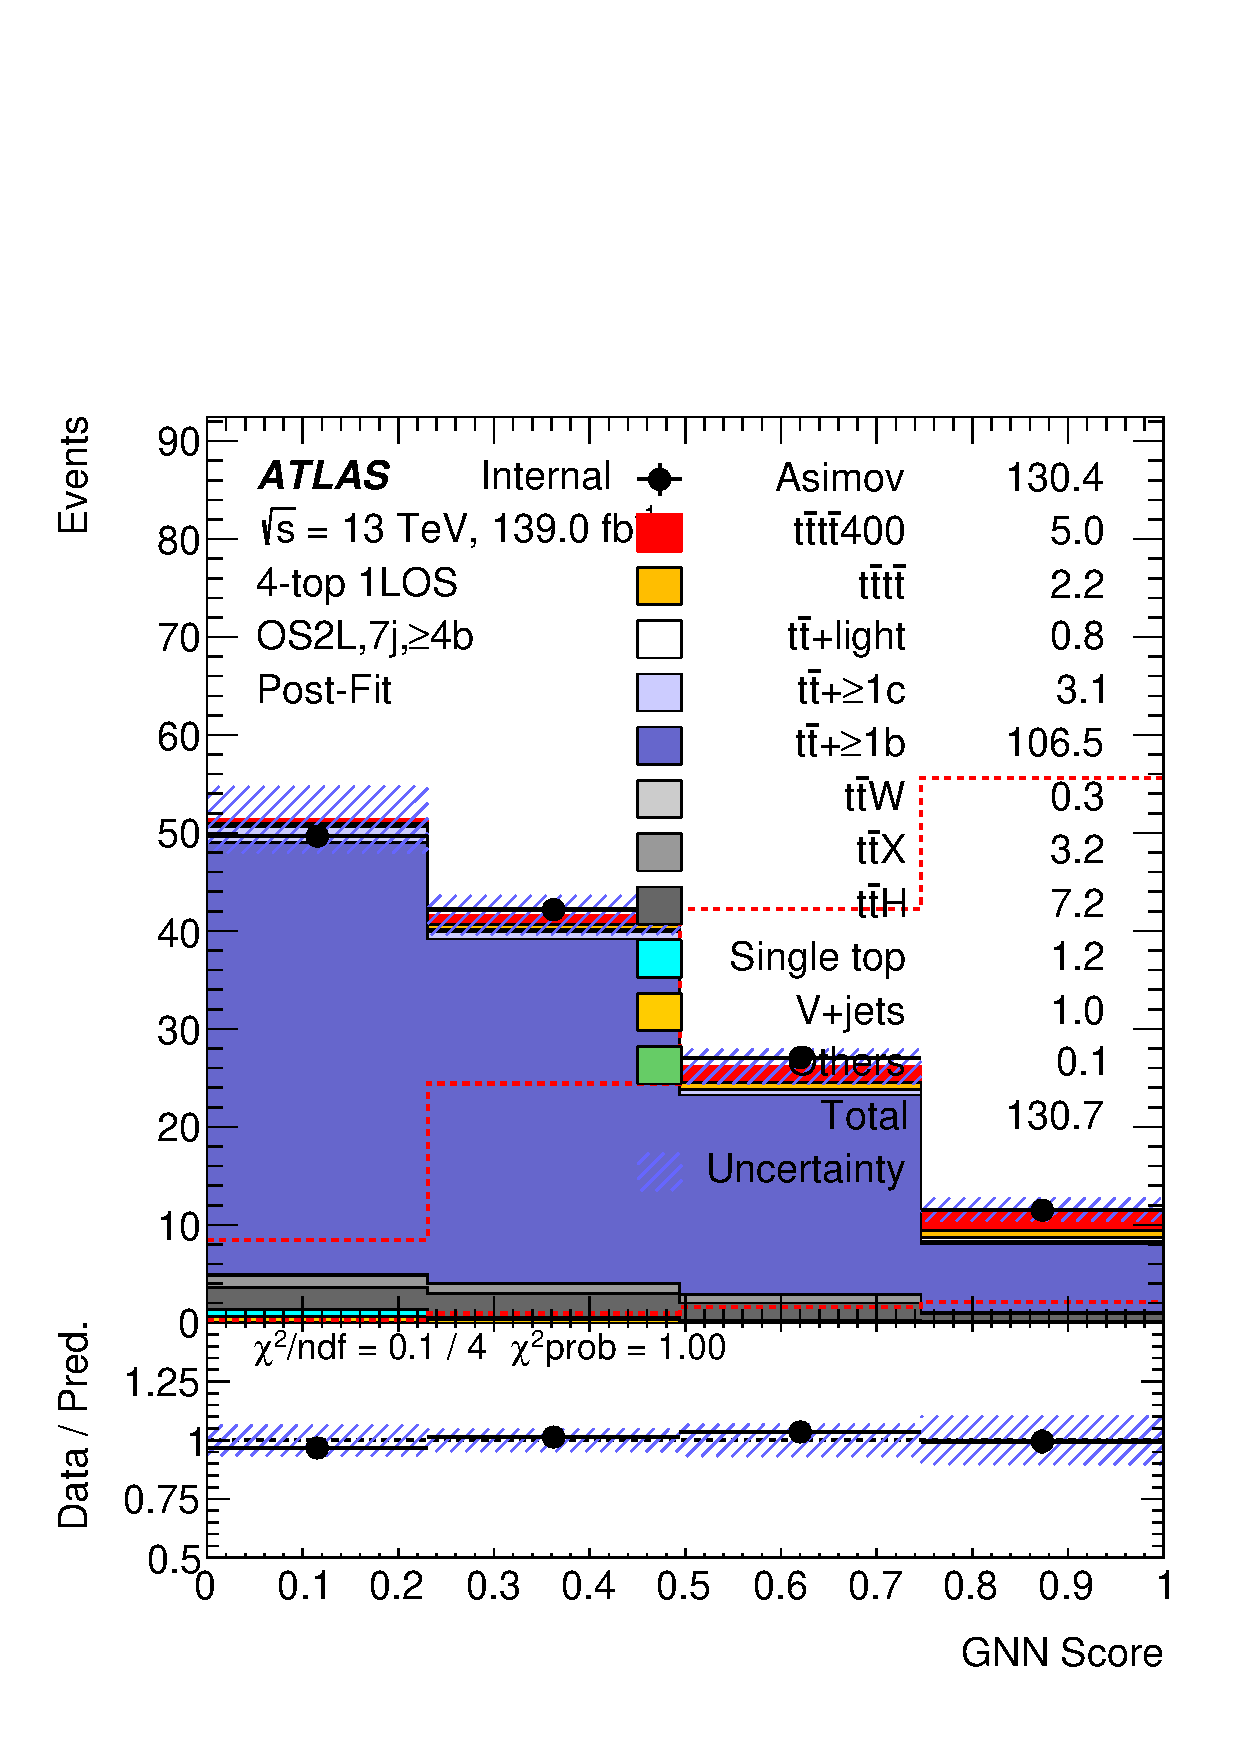
\includegraphics[width=0.31 \textwidth]{figures/4FS_studies/dataMC_4FSsyst_norew/os2l_7jge4b_postFit.pdf} \\

        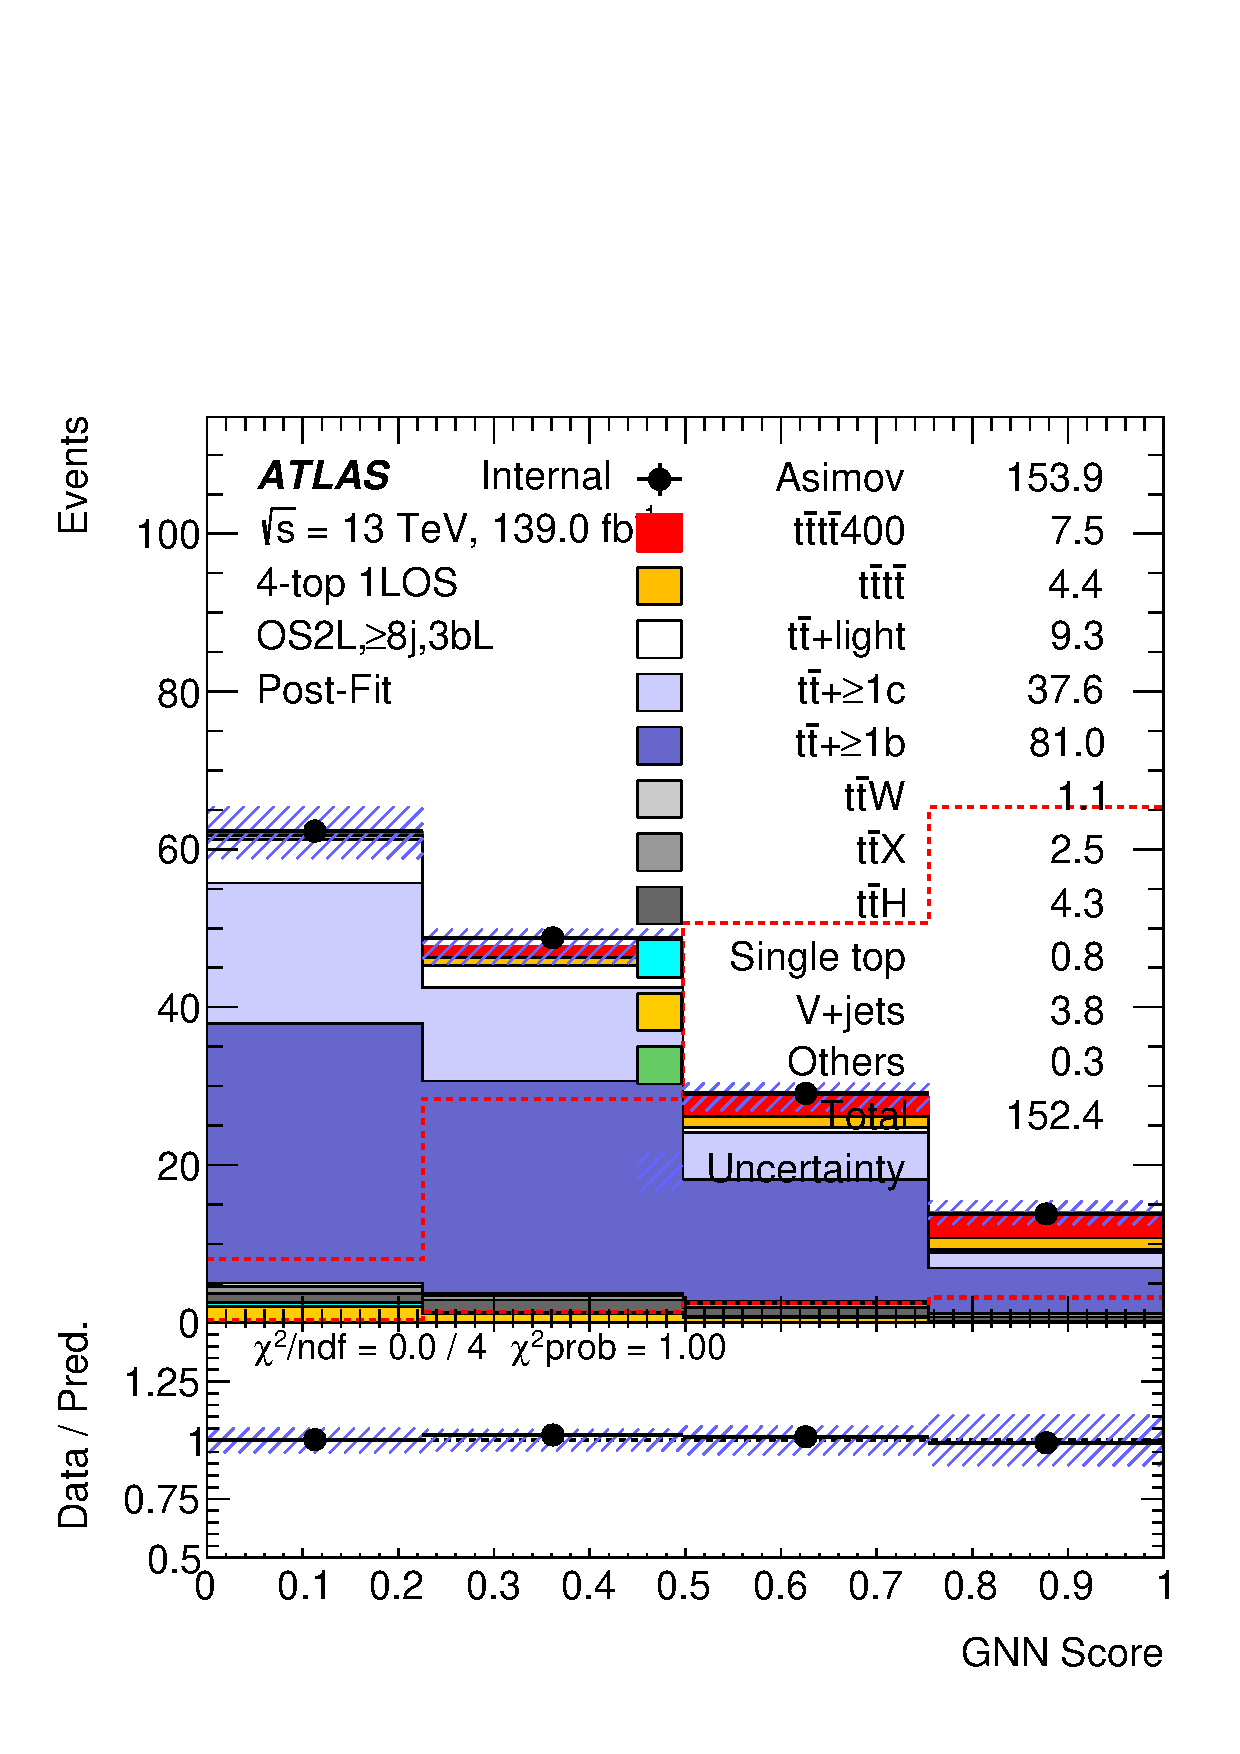
\includegraphics[width=0.31 \textwidth]{figures/4FS_studies/dataMC_4FSsyst_norew/os2l_ge8j3bL_postFit.pdf} &
        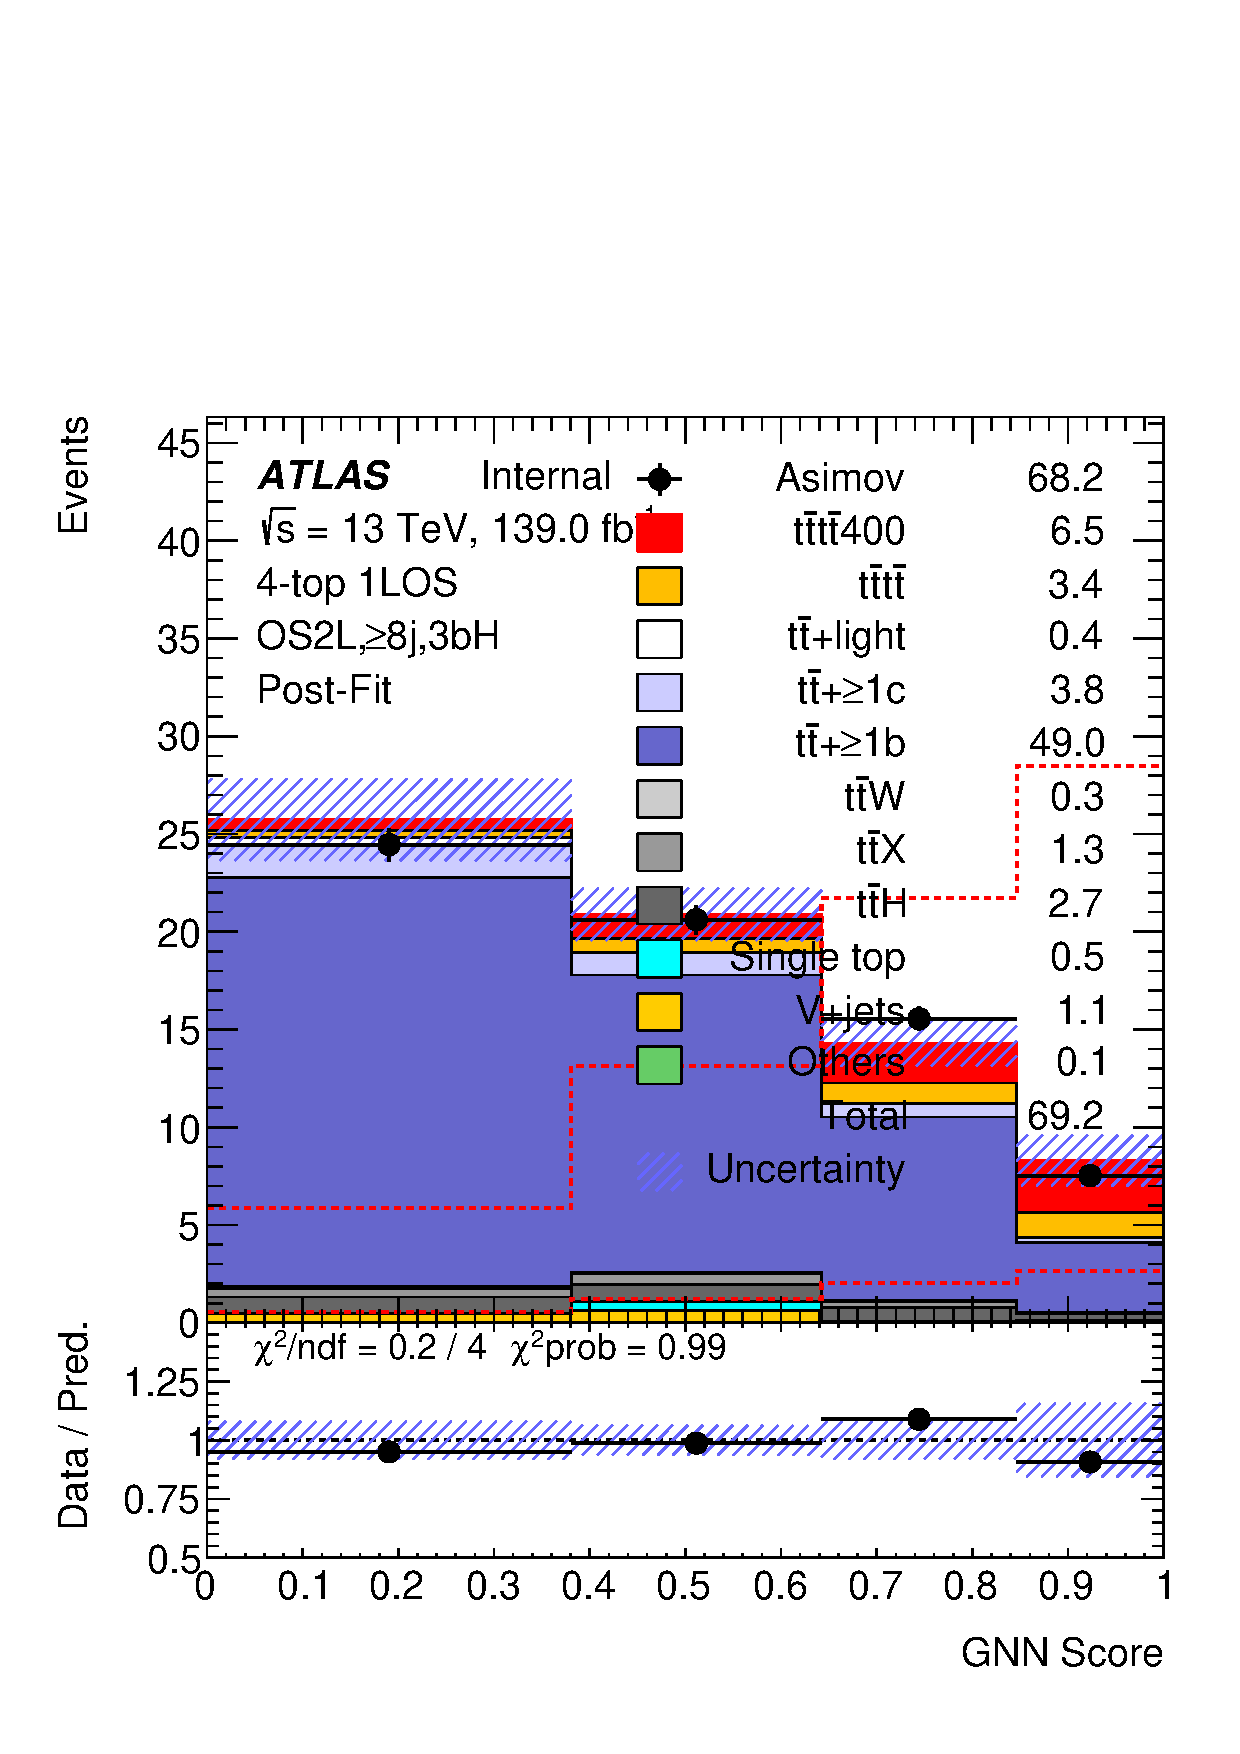
\includegraphics[width=0.31 \textwidth]{figures/4FS_studies/dataMC_4FSsyst_norew/os2l_ge8j3bH_postFit.pdf} &
        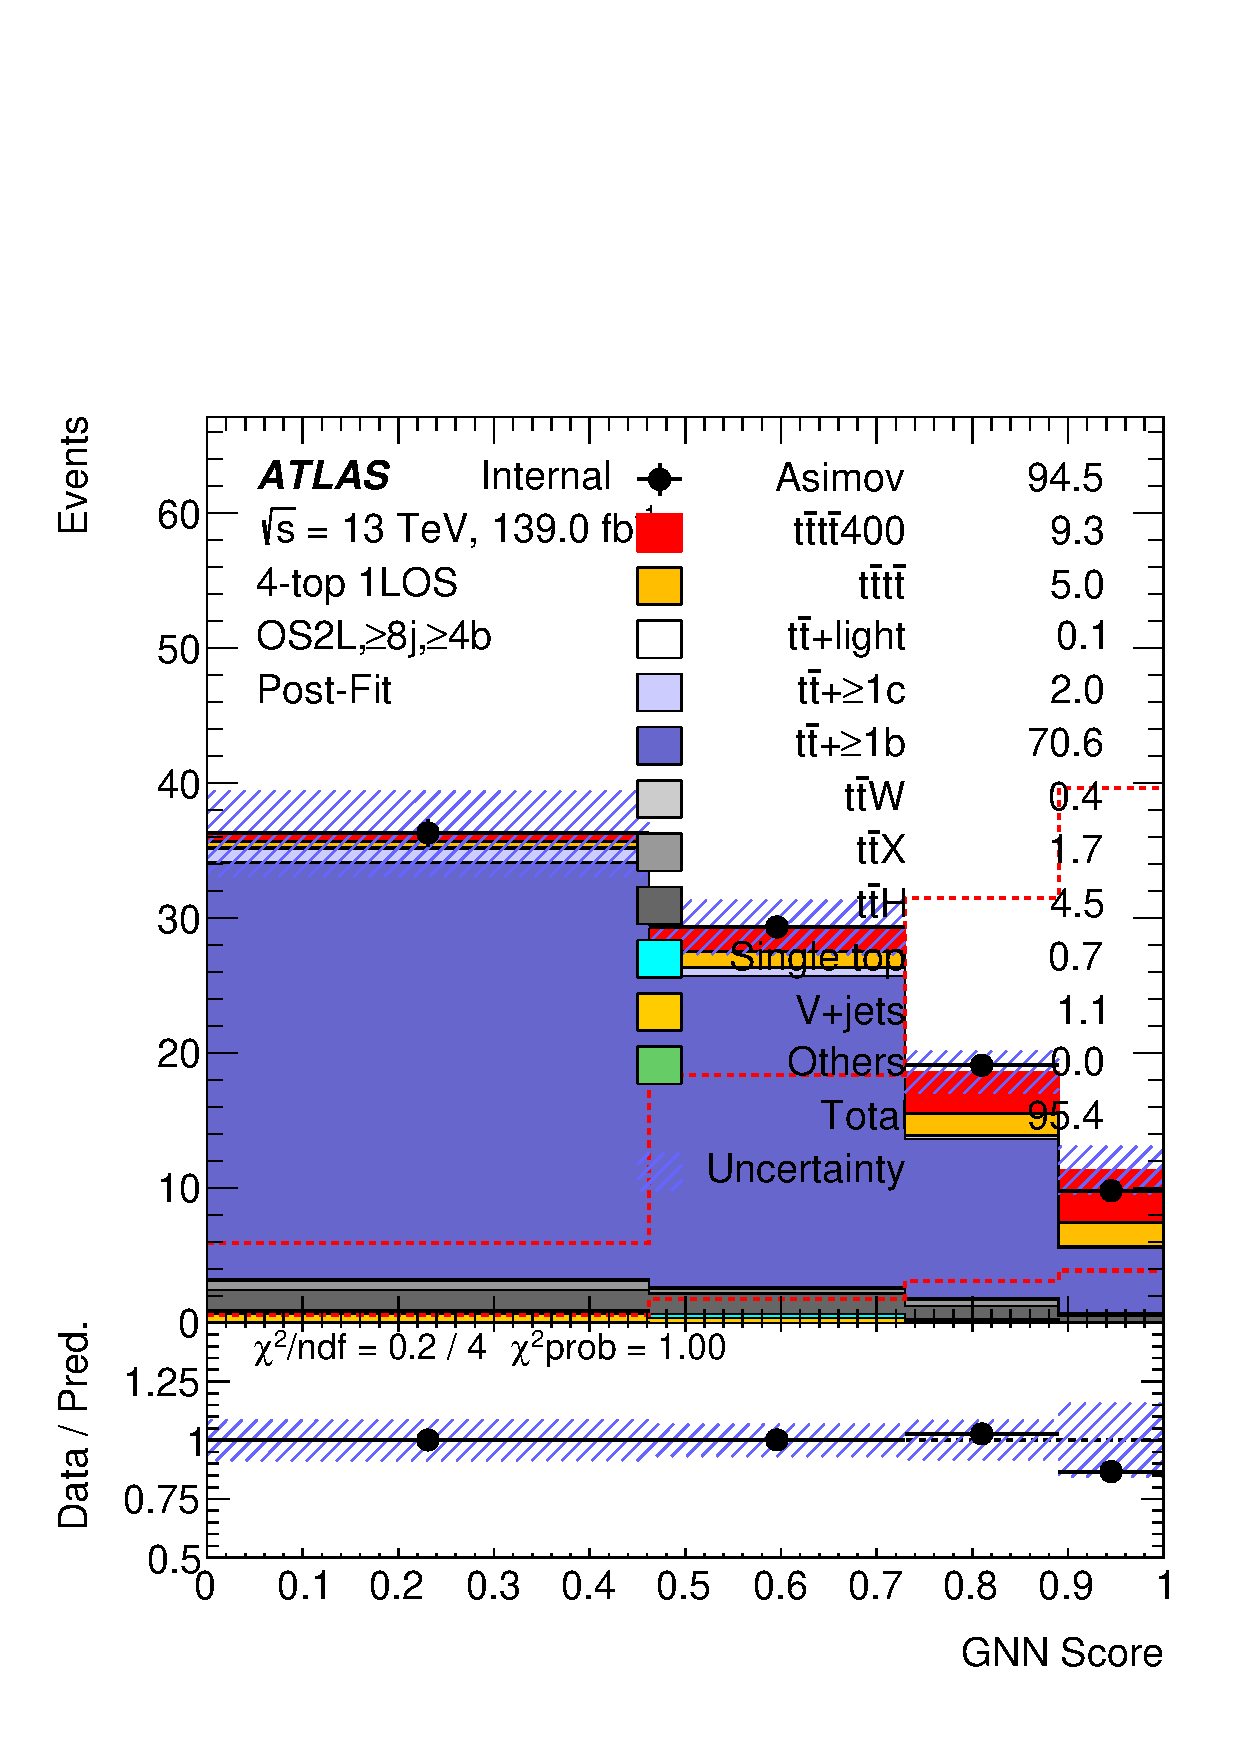
\includegraphics[width=0.31 \textwidth]{figures/4FS_studies/dataMC_4FSsyst_norew/os2l_ge8jge4b_postFit.pdf} \\
        \end{tabular}
        \caption{\label{fig:4FS_dataMC_4FSsyst_norew_2L_postfit}Post-fit comparison of the 2LOS regions between samples with $t\bar{t}$ TTB samples produced with 5FS (MC) and $t\bar{t}$ TTB samples produced with 4FS (set as `pseudodata'). All systematics including 4FS systematics are incorporated in the uncertainty. The $t\bar{t}$ samples are not reweighted.}
\end{center}
\end{figure}


\begin{figure}[htbp!]
  \centering
  \begin{subfigure}[t]{\textwidth}
    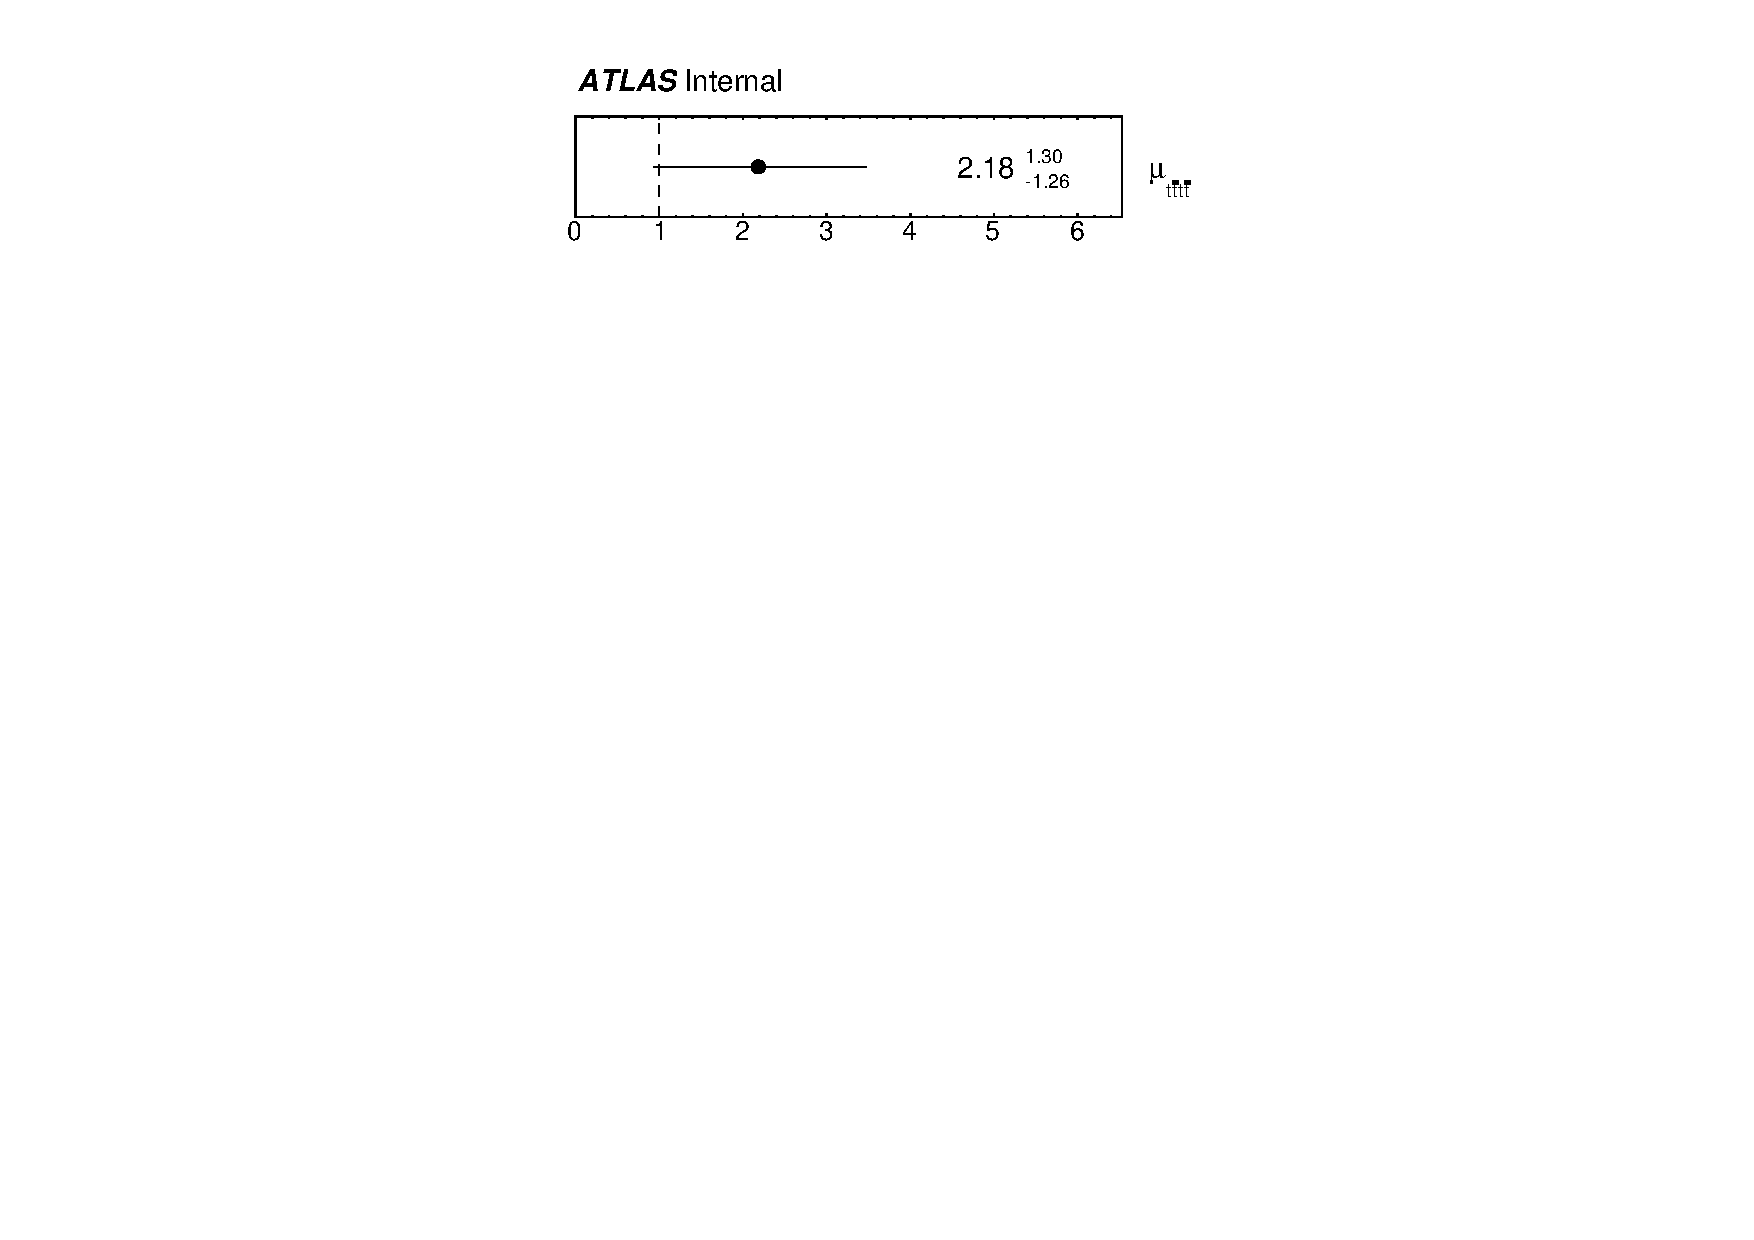
\includegraphics[width=\linewidth]{figures/4FS_studies/dataMC_4FSsyst_norew/NormFactors.pdf}
     \caption{\label{fig:4FS_dataMC_NormFactors_syst}with FS syst, without $t\bar{t}$ reweighting}
  \end{subfigure}
  \begin{subfigure}[t]{\textwidth}
    
\includegraphics[width=\linewidth]{figures/4FS_studies/dataMC_syst_rew/NormFactors.pdf}
     \caption{\label{fig:4FS_dataMC_NormFactors_syst}without FS syst }
  \end{subfigure}
  \begin{subfigure}[t]{\textwidth}
    
\includegraphics[width=\linewidth]{figures/4FS_studies/dataMC_4FSsyst_rew/NormFactors.pdf}
     \caption{\label{fig:4FS_dataMC_NormFactors_FSsyst}with FS syst }
  \end{subfigure}
  \caption{\label{fig:4FS_dataMC_NormFactors}Signal strength ${\mu}_{t\bar{t}t\bar{t}}$ extracted from the fit of 5FS MC to 4FS 'pseudodata.' The value corresponding to no discrepancy between 4FS and 5FS is ${\mu}_{t\bar{t}t\bar{t}} = 1$. The fit without 4FS systematics does not reach this value, but the fit when including 4FS systematics does within uncertainties.}
\end{figure}

\begin{figure}[htbp!]
  \centering
  \begin{subfigure}[t]{0.32\textwidth}
    
\includegraphics[width=\linewidth]{figures/4FS_studies/dataMC_syst_rew/NuisPar_comp.pdf}
    \subcaption{with 4FS systematics vs without}
    \label{fig:4FS_dataMC_NuisPar_4FSvsno4FS}
  \end{subfigure}
  \begin{subfigure}[t]{0.32\textwidth}
    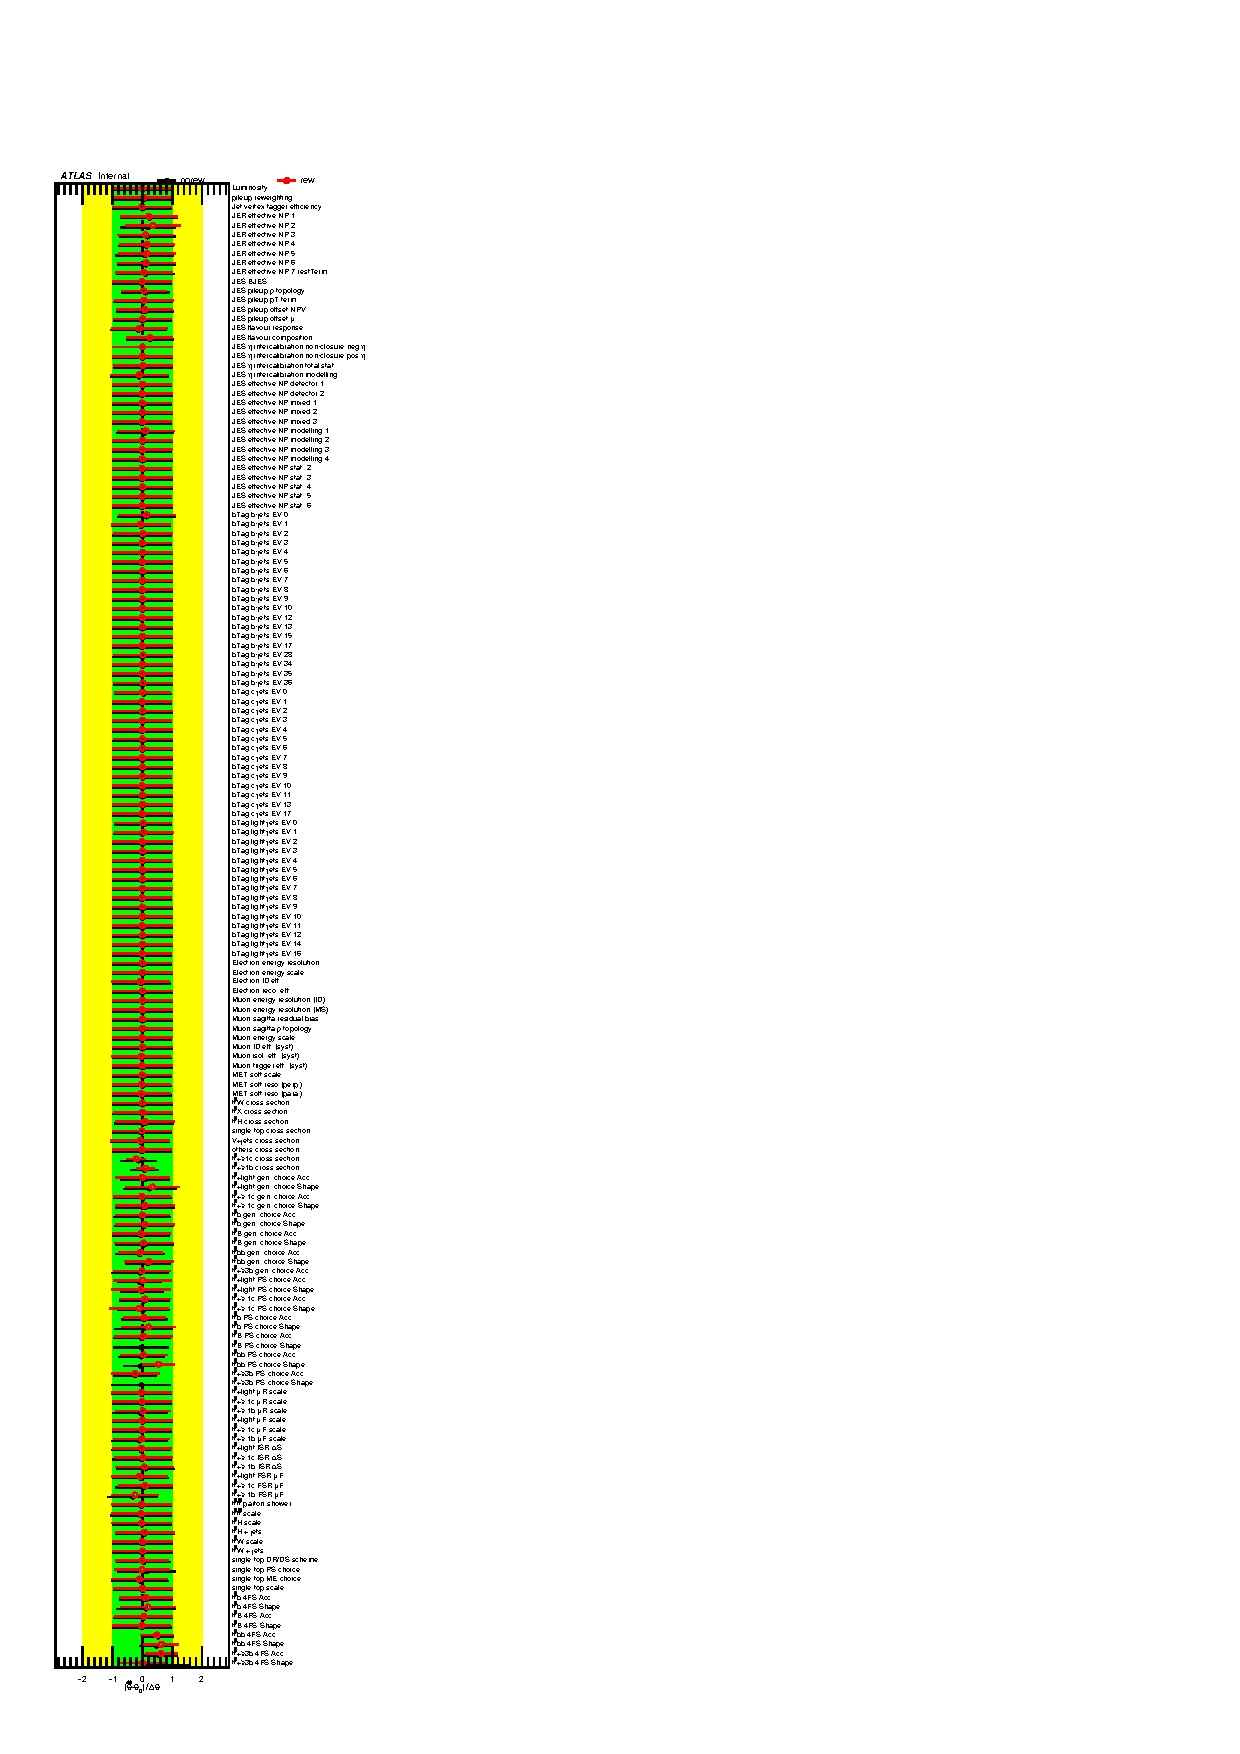
\includegraphics[width=\linewidth]{figures/4FS_studies/dataMC_4FSsyst_norew/NuisPar_comp.pdf}
    \subcaption{with 4FS systematics, with $t\bar{t}$ rew vs without}
    \label{fig:4FS_dataMC_NuisPar_rewvsnorew}
  \end{subfigure}
  \caption{\label{fig:4FS_dataMC_NuisPar_comp}Comparison of NP pulls and constraints when using 4FS systematics versus without. Comparison of NP pulls and constraints when using 4FS systematics, with $t\bar{t}$ reweighting versus without.}
\end{figure}
